%\chapter{Beam Normal Single Spin Asymmetry in Inelastic Scattering}
\chapter{BEAM NORMAL SINGLE SPIN ASYMMETRY}
\label{BEAM NORMAL SINGLE SPIN ASYMMETRY}

%%%%%%%%%%%%%%%%%%%%%%%%%%%%%%%%%%%%%%%%%%%%%%%%%%%%%%%%%%%%%
\section{Introduction}
\label{Introduction}

Dedicated measurements of the beam normal single spin asymmetry in inelastic electron-proton, and electron-nucleus scattering near missing mass, $W$, $\sim$1.2~GeV were performed during 18 - 20 February 2012 at Hall-C of Jefferson Lab using Q-weak apparatus. 

%%%%%%%%%%%%%%%%%%%%%%%%%%%%%%%%%%%%%%%%%%%%%%%%%%%%%%%%%%%%%%
%\section{Experimental Method}
%\label{Experimental Method}
%
The Q-weak longitudinal measurement setup~\cite{qweak_proposal_2007} was used for an inelastic transverse measurement. The electron beam polarization was changed from the nominal longitudinal setup to produce fully horizontal/ vertical polarization using the double Wien filter at the injector (section~\ref{Polarized Source and Helicity Reversal}). The torodial magnet setting was lowered to 6700~A to focus inelastically scattered electrons onto the main \v{C}erenkov detectors. 


\begin{figure}[!h]
	\begin{center}
	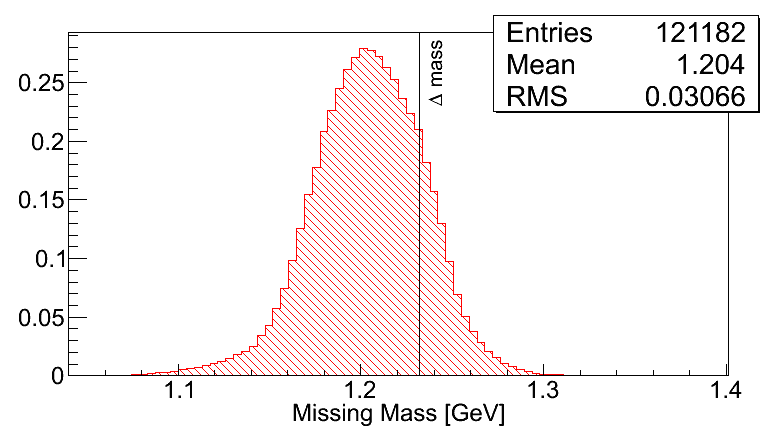
\includegraphics[width=10.0cm]{figures/W_G3}
	\end{center}
	\caption
%	[Simulated missing mass, W, distribution at the inelastic QTor setting.]	
	{Simulated missing mass, W, distribution at the inelastic QTor setting.}
	\label{fig:W_G3}
\end{figure}

%%%%%%%%%%%%%%%%%%%%%%%%%%%%%%%%%%%%%%%%%%%%%%%%%%%%%%%%%%%%%
\section{Available Data Set and Conditions of Experimental Data Taking}
\label{Available Data Set and Conditions of Experimental Data Taking}

The total collected data after hardware and software quality cuts is shown in Table~\ref{tab:transverse_inelastic_data_set}. The QTor current of 6700~A selects the inelastic events near $W\sim$1.2~GeV (Figure~\ref{fig:W_G3}). Data on both sides of the inelastic peak (6000~A and 7300~A) were taken to better constrain the elastic dilution. Two transverse spin orientations, horizontal and vertical, were used. Data were collected on a liquid hydrogen (LH$_{2}$) cell, 4\% thick downstream aluminum alloy (Al), and a 1.6\% thick downstream carbon foil ($^{12}$C) with 1.155~GeV beam for both spin orientations. 
%Vertical transverse are shown in parenthesis, rest are for horizontal transverse.
Different beam currents were used on different targets (see Table~\ref{tab:transverse_inelastic_data_set}).
The beam was rastered on the target over an area of 4~mm$\times$4~mm by the fast raster system to minimize the target boiling or damage.
The Insertable Half Wave Plate (IHWP) was used to help suppress helicity correlated beam asymmetries and was reversed at intervals of about 2~hours. 
More information about the conditions of data taking is given in APPENDIX-\ref{Beam Normal Single Spin Asymmetry in Inelastic e-p Scattering} section~\ref{Condition of Experimental Data Taking}.


%\renewcommand\arraystretch{2.4} 
%\setlength\minrowclearance{2.4pt}
\renewcommand{\arraystretch}{1.0} % make cell wider
\begin{table}[!h]
 \begin{center}
   \caption
%	[The transverse N$\rightarrow\Delta$ data set.]   
	{The transverse N$\rightarrow\Delta$ data set. The runs with vertical transverse polarization are in parentheses, the rest are from horizontal transverse polarization. Data collected in an hour was defined as run. The beam currents are shown in second to last row. Total charge on target in Coulombs is shown in the bottom row.}
  \begin{tabular}{ c | c | c  c  c | c  c }
%    \hline
    \noalign{\hrule height 1pt}
%    \multirow{2}{*}{HWP} & QTor current  & & QTor current & &  \multicolumn{2}{c}{QTor current} \\
    \multirow{3}{*}{IHWP} & \multicolumn{6}{c}{QTor current} \\ \cline{2-7}
%	\cline{2-7}%\hline
		 &  6000 A & & 6700 A & &  \multicolumn{2}{c}{7300 A}\\
	\cline{2-7}%\hline
	     & LH$^{\dagger}_{2}$ & LH$^{\dagger}_{2}$ & Al$^{\dagger\dagger}$ & $^{12}$C &  LH$^{\dagger}_{2}$ & Al$^{\dagger\dagger}$ \\
%	\cline{2-7}%\hline
    \noalign{\hrule height 1pt}
%    \hline
	IN  & \pbox{3cm}{16152\\ 16153} & \pbox{3cm}{(16066)\\ 16131\\ 16132} & \pbox{3cm}{(16067)\\ 16115\\ 16116} & \pbox{3cm}{16150\\ 16151} & \pbox{3cm}{16133\\ 16134\\ 16135} & \pbox[c][2cm][c]{3cm}{ 16122\\ 16123\\ 16124\\ 16160 } \\ 
    \noalign{\hrule height 1pt}
%	\hline
	OUT & \pbox{5cm}{16154\\ 16156\\ 16157\\ 16158} & \pbox{5cm}{(16065)\\ 16129\\ 16130} & \pbox{5cm}{\vspace{5pt}(16068)\\ (16069)\\ 16117\\ 16118\\ 16119\vspace{5pt}} & \pbox{5cm}{16148\\ 16149} & \pbox{5cm}{16136\\ 16137} & \pbox{5cm}{16120\\ 16121\\ 16161} \\ 
%    \hline
    \noalign{\hrule height 1pt}
	   Beam current $I$ [$\mu$A] & 180 & 180 & 60 & 75 & 180 & 60 \\
    \noalign{\hrule height 1pt}
%	\hline
	   Collected Data [C] & 1.5 & 1.8 (1.9) & 0.8 (0.4) & 0.6 & 2.0 & 0.9 \\
%	\hline
    \noalign{\hrule height 1pt}
   \end{tabular}
 \label{tab:transverse_inelastic_data_set}
 \end{center}
\end{table}
\renewcommand{\arraystretch}{1.0} % make cell wider

In this dissertation, a full analysis of the beam normal single spin asymmetry from inelastic electron-proton scattering on LH$_{2}$ target, indicated by $\dagger$ in Table~\ref{tab:transverse_inelastic_data_set}, will be discussed. The transverse asymmetry on Al target, indicated by $\dagger\dagger$ in the table, was also analyzed as a background correction for the LH$_{2}$ target. The analysis of the remaining data are ongoing and will not be covered in this dissertation.

%%%%%%%%%%%%%%%%%%%%%%%%%%%%%%%%%%%%%%%%%%%%%%%%%%%%%%%%%%%%%
\section{Extraction of Raw Asymmetries}
\label{Extraction of Raw Asymmetries}

A single detector asymmetry was obtained by averaging the two PMT asymmetries from each \v{C}erenkov detector. The error weighted average of the asymmetries from runlets, $\sim$5 minute long data samples, was extracted for a given data set. To extract the raw asymmetry $A_{\rm raw}$ from the detectors, the average asymmetry for the two different Insertable Half Wave Plate (IHWP) settings, IN and OUT, were determined separately for each main detector bar. The asymmetries measured in the IHWP configurations were sign corrected for the extra spin flip and averaged together after checking for the IHWP cancellation of the false asymmetries. The error weighted value of $<$IN,-OUT$>$ determined the measured raw asymmetry for each bar. These raw asymmetries were then plotted against the detector octant number, which represents the location of the detector in the azimuthal plane ($\phi$ = (octant - 1)$\times$45$^{\circ}$), and they were fitted using a function of the form in Equation~\ref{equ:eqFitTransverse}.
This analysis will focus on the azimuthal dependence of the detector asymmetries representing the transverse asymmetries.

\begin{equation} \label{equ:eqFitTransverse}
f(\phi) = \left\lbrace 
\begin{aligned}
\text{Horizontal transverse:}~\epsilon_{M}^{H} \sin(\phi + \phi_{0}^{H}) + C^{H}\\
\text{Vertical transverse:}~\epsilon_{M}^{V} \cos(\phi + \phi_{0}^{V}) + C^{V}.
\end{aligned}
\right.
\end{equation}

Here, $\phi$ is the azimuthal angle in the transverse plane to the beam direction. $\phi$ = 0 indicates beam left, $\phi_{0}$ is a possible phase offset expected to be consistent with zero. $\epsilon_{M}$ is the measured asymmetry (amplitude) of the azimuthal modulation generated by BNSSA, and $C$ is a constant appearing for monopole asymmetries such as the parity violating asymmetry generated by residual longitudinal polarization in the beam. The measured un-regressed raw asymmetries for the horizontal and vertical transverse polarization on LH$_{2}$ target are $\epsilon_{\rm raw}^{H}$ = 5.34~$\pm$~0.53~ppm and $\epsilon_{\rm raw}^{V}$ = 4.60~$\pm$~0.81~ppm, respectively. 

%\begin{center}
%\framebox[\frameboxsize][c]{Combined (error weighted) asymmetry $A_{M}^{in}$ is 5.095$\pm$0.444~ppm.}
%\end{center}


\begin{figure}[!h]
	\begin{center}
	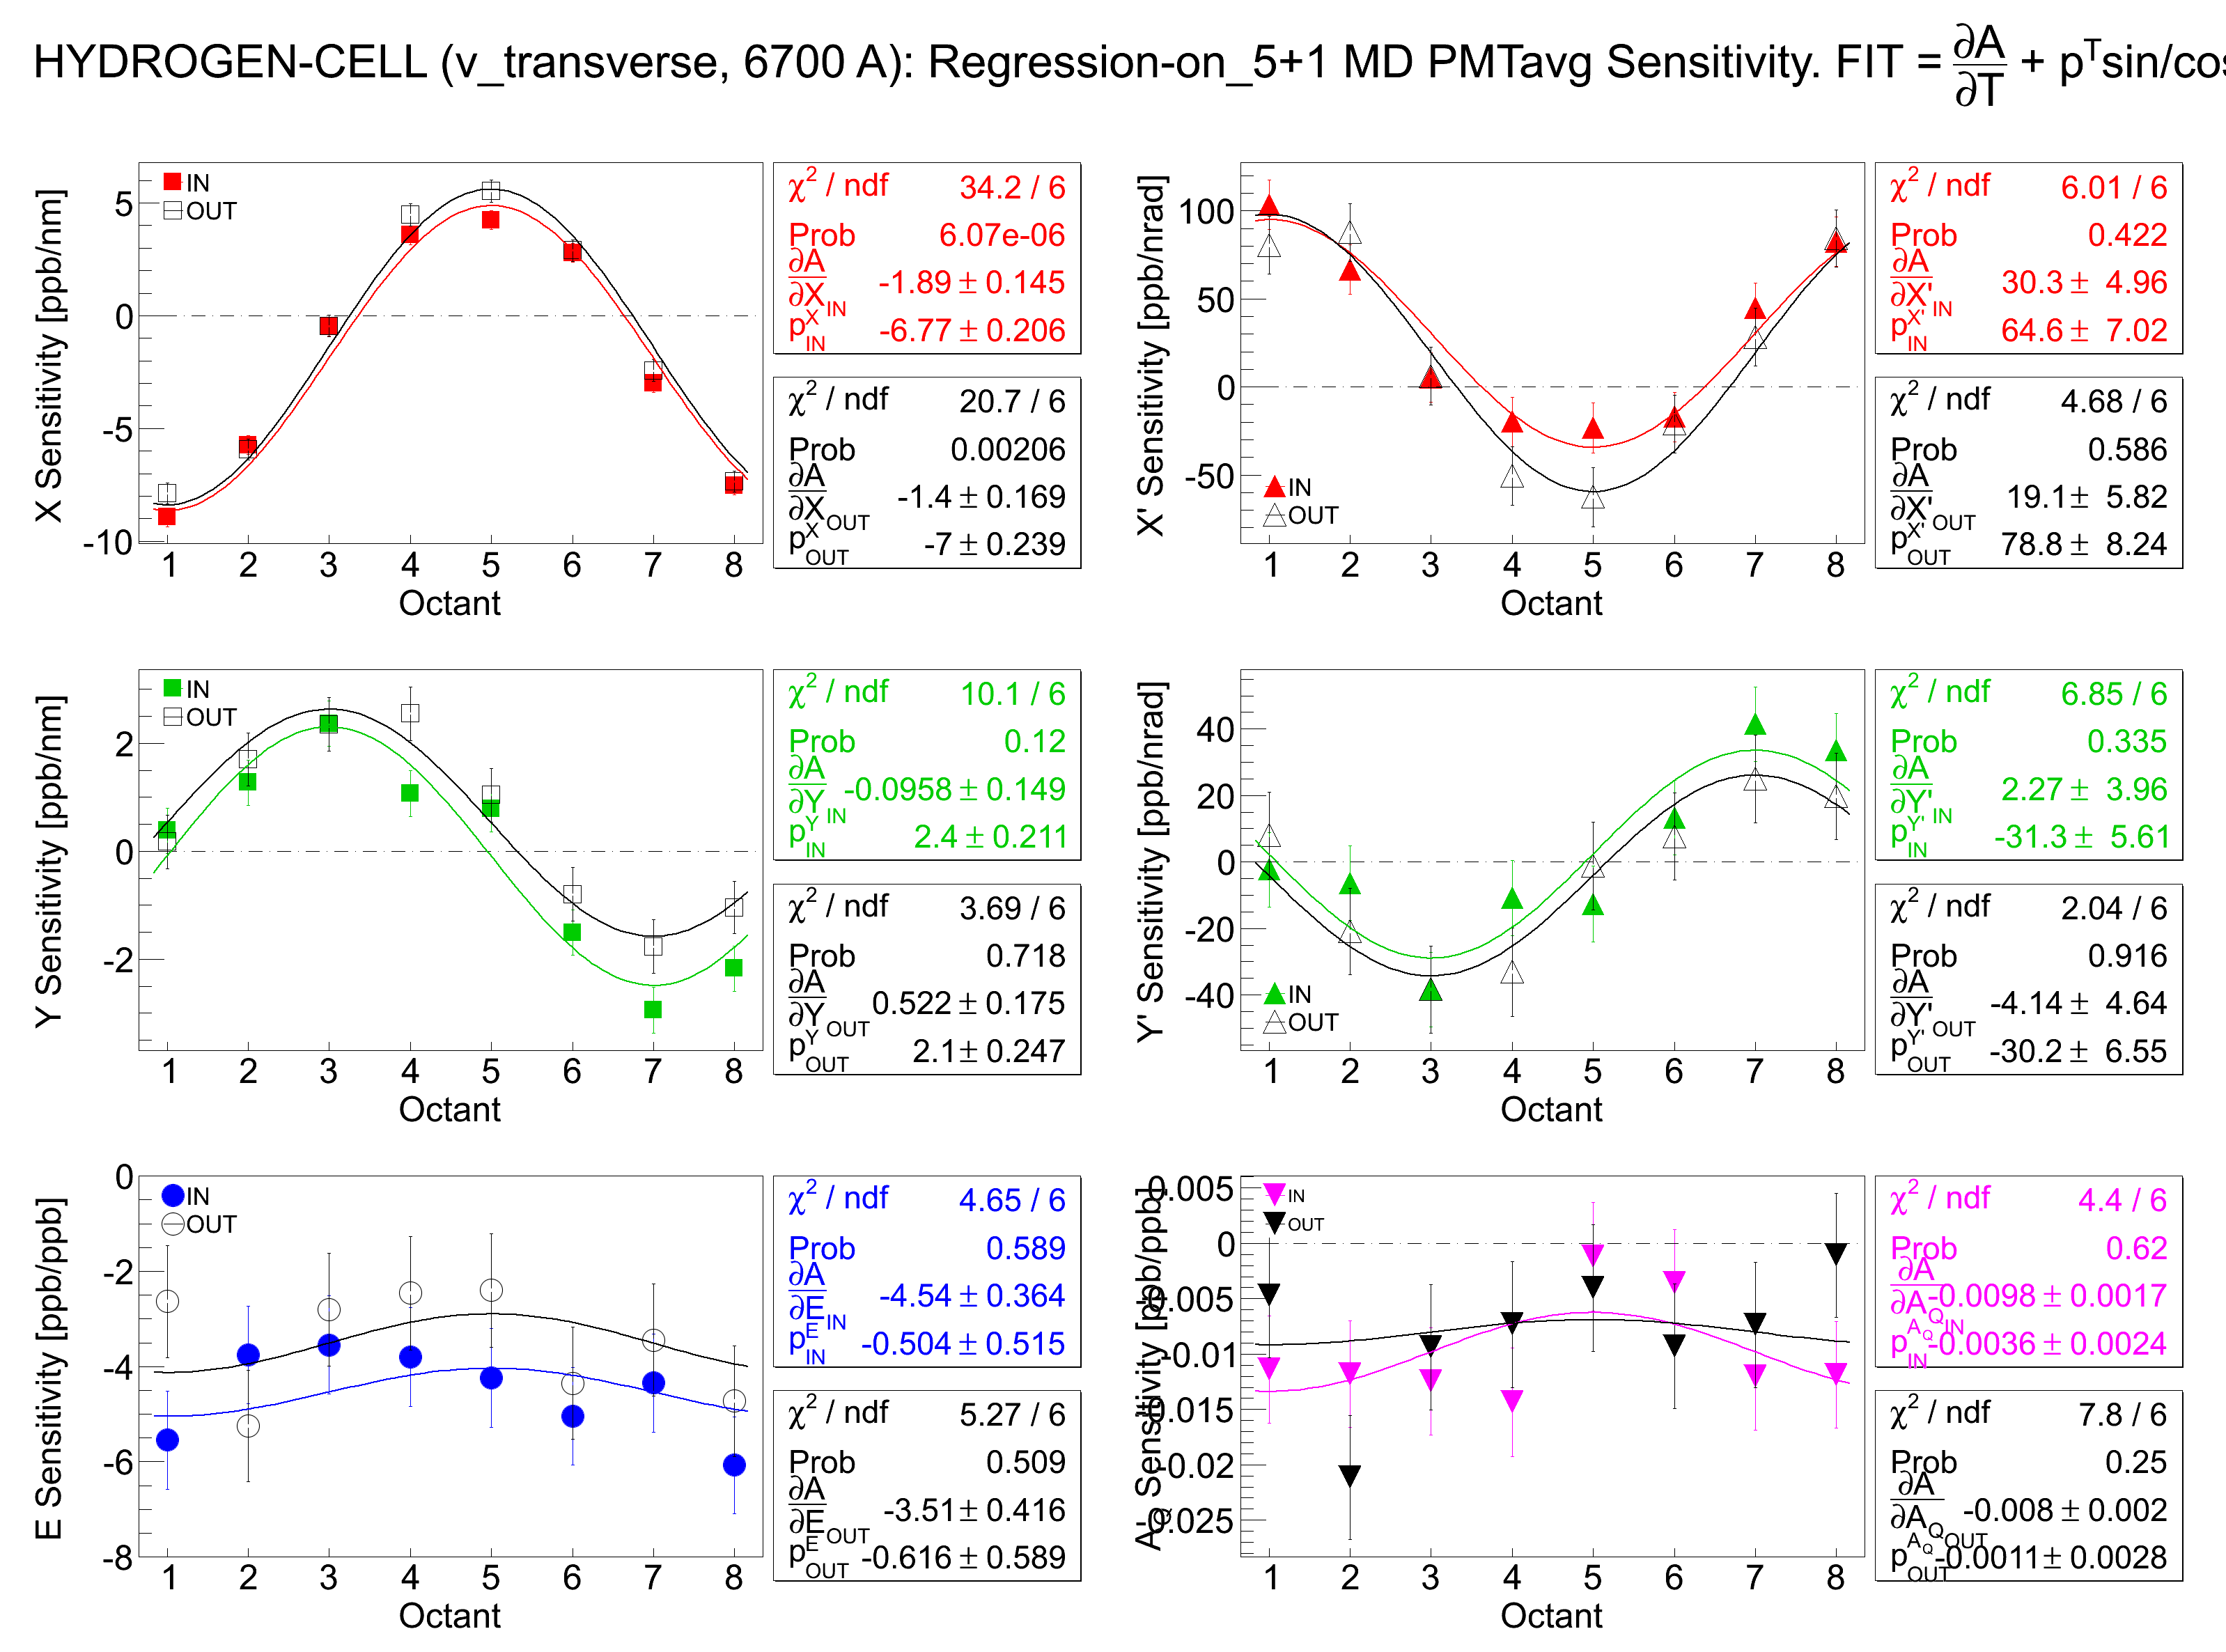
\includegraphics[width=15.0cm]{figures/MD_v_transverse_5+1_Sensitivities}
	\end{center}
	\caption
%	[Azimuthal dependence of the main detector sensitivities to HCBA in the vertical LH$_{2}$ transverse data set.]	
	{Azimuthal dependence of the main detector sensitivities to HCBA for the ``5+1" regression scheme in the vertical LH$_{2}$ transverse data set are shown here. Sensitivities for beam positions and angles have sinusoidal dependence with octant. No such strong dependence is seen for energy and charge. Two IHWP states are shown separately for each beam parameter. Fit functions used to fit the parameters are shown on the plot. The constant in the fit gives the error weighted average of the sensitivities. See APPENDIX-\ref{Beam Normal Single Spin Asymmetry in Inelastic e-p Scattering}, section~\ref{Corrections}  for the sensitivities and corrections from full data sets.}
	\label{fig:MD_v_transverse_5+1_Sensitivities}
\end{figure}


%%%%%%%%%%%%%%%%%%%%%%%%%%%%%%%%%%%%%%%%%%%%%%%%%%%%%%%%%%%%%
\section{Asymmetry Correction using Linear Regression}
\label{Asymmetry Correction using Linear Regression}

The helicity correlated changes in the electron beam position, angle, and energy change the yield of the electrons in the detector acceptance. This can create false asymmetries in the detector and needs to be corrected before the extraction of the physics asymmetry. A multi-variable linear regression~\cite{linRegTechNote} is used to remove the beam asymmetries from the raw \v{C}erenkov detector asymmetries as shown in Equation~\ref{equ:regression}.

\begin{equation} \label{equ:regression}
\epsilon_{M} = \epsilon_{\rm raw} - \sum^{6}_{i=1} \left(\frac{\partial \epsilon_{\rm raw} }{ \partial T_{i} }\right) \Delta T_{i}
\end{equation}

Here $\epsilon_{M}$ is the measured asymmetry after regression, and ($\partial \epsilon_{\rm raw}/\partial T_{i}$) is the detector sensitivity to a helicity-correlated beam parameter $T_{i}$ with helicity-correlated differences $\Delta T_{i}$. During this measurement period, the helicity-correlated differences were fairly stable except for charge (shown in Figures~\ref{fig:transverse_LH2_h_diff}, and~\ref{fig:transverse_LH2_v_diff}, APPENDIX~\ref{Beam Normal Single Spin Asymmetry in Inelastic e-p Scattering}) and are summarized in Figure~\ref{fig:differences_6700_LH2_off_on_5+1} and Table~\ref{tab:differences}. The detector sensitivity slopes are calculated with linear regression, which uses natural beam motion during a runlet and considers correlations between different beam parameters. The asymmetries presented in this dissertation are regressed against six ``5+1" beam parameters ($T_{i}$): horizontal position ($X$), horizontal angle ($X^{\prime}$), vertical position ($Y$), vertical angle ($Y^{\prime}$), the energy asymmetry ($A_{E}$), and the charge asymmetry ($A_{Q}$). The sensitivities of the \v{C}erenkov detectors to different helicity correlated beam parameters have azimuthal dependence, as shown in Figure~\ref{fig:MD_v_transverse_5+1_Sensitivities} (shown for vertical transverse data only, horizontal transverse can be found in Figure~\ref{fig:MD_h_transverse_5+1_Sensitivities}). This azimuthal dependence of the position and angle sensitivities are a result of the movement of the scattered electron profile across the octants which changes the effective scattering angle of the detected electrons not specific to the transverse asymmetry measurement. The position and angle sensitivities are anti-correlated. The energy and charge sensitivities are not expected to have a strong azimuthal dependence since they do not change the acceptance. The size of the applied correction to the raw asymmetries depends on the size of the helicity-correlated beam parameter differences $\Delta T_{i}$ and the sensitivities ($\partial \epsilon_{\rm raw}/\partial T_{i}$). The size of the corrections were $\sim$2-3 orders of magnitude smaller than the size of the measured asymmetry and are shown in Figure~\ref{fig:MD_v_transverse_5+1_corrections} (shown for vertical transverse data only, horizontal transverse can be found in Figure~\ref{fig:MD_h_transverse_5+1_corrections}). The total applied regression correction (Figure~\ref{fig:MD_v_transverse_5+1_TotalCorrections}) is dominated by the $X$ correction (Figure~\ref{fig:MD_v_transverse_5+1_corrections} top left). The corrections are summarized in Figure~\ref{fig:correctionSummary_LH2}.

%\begin{table}[!h]
%\begin{center}
%  	\caption
%	[Beam parameter differences for the Hydrogen horizontal and vertical transverse data sets.] 
%  	{Beam parameter differences for the Hydrogen horizontal and vertical transverse data sets. The X differences are higher compared to Y differences.}
%  \begin{tabular}{ c | c  c | c  c }
%%	\hline
%    \noalign{\hrule height 1pt}
%    Beam parameter & \multicolumn{2}{c|}{Horizontal} & \multicolumn{2}{c}{Vertical} \\ 
%    \cline{2-5}
%%	\hline
%    	differences &	IHWP IN	&	IHWP OUT &	 IHWP IN	&	IHWP OUT  \\
%%	\hline
%    \noalign{\hrule height 1pt}
%	$\Delta$X~[nm] & 23.8~$\pm$~2.1 & 20.6~$\pm$~2.3 & 15.4~$\pm$~3.1	& 58.0~$\pm$~3.6\\
%	$\Delta$Y~[nm]	& 6.9~$\pm$~2.1 & 5.6~$\pm$~2.3 & 20.2~$\pm$~3.1 & 15.4~$\pm$~3.6 \\
%	$\Delta$X$^{\prime}$~[nrad] & 0.7~$\pm$~0.1 & 0.7~$\pm$~0.1 & 0.6~$\pm$~0.2	& 1.3~$\pm$~0.2\\
%	$\Delta$Y$^{\prime}$~[nrad] & 0.2~$\pm$~0.1 & -0.3~$\pm$~0.1 & 0.6~$\pm$~0.2	& 0.9~$\pm$~0.2\\
%	$\Delta$E~[ppb]	& -2.3~$\pm$~2.1 & -1.5~$\pm$~2.3 & 0.5~$\pm$~3.1	& -5.4~$\pm$~3.6\\
%	$\Delta$A$_{Q}$~[ppb]	& 8.2~$\pm$~0.5 & -237.3~$\pm$~55.6 & 60.1~$\pm$~0.7	& 158.1~$\pm$~88.1\\
%%	\hline
%    \noalign{\hrule height 1pt}
%  	\end{tabular}
%  \label{tab:differences}
%\end{center}
%\end{table}

%\begin{table}[!h]
%\begin{center}
%  	\caption
%	[Beam parameter differences for the Hydrogen horizontal transverse data set.] 
%  	{Beam parameter differences for the Hydrogen horizontal transverse data set. The X differences are higher compared to Y differences.}
%  \begin{tabular}{ c | c  c  c  c }
%%	\hline
%    \noalign{\hrule height 1pt}
%    Beam parameter & \multirow{2}{*}{IHWP IN}	&	\multirow{2}{*}{IHWP OUT} &	 \multirow{2}{*}{($<$IN$>$+$<$OUT$>$)/2}	&	\multirow{2}{*}{($<$IN$>$,-$<$OUT$>$)} \\ 
%%	\hline
%    	differences &  &  & & \\
%%	\hline
%    \noalign{\hrule height 1pt}
%	$\Delta$X~[nm] & 23.8~$\pm$~2.1 & 20.6~$\pm$~2.3 & 22.2~$\pm$~1.6	& 3.6~$\pm$~1.6\\
%	$\Delta$Y~[nm]	& 6.9~$\pm$~2.1 & 5.6~$\pm$~2.3 & 6.2~$\pm$~1.6 & 1.2~$\pm$~1.6 \\
%	$\Delta$X$^{\prime}$~[nrad] & 0.7~$\pm$~0.1 & 0.7~$\pm$~0.1 & 0.7~$\pm$~0.1	& 0.1~$\pm$~0.1\\
%	$\Delta$Y$^{\prime}$~[nrad] & 0.2~$\pm$~0.1 & -0.3~$\pm$~0.1 & -0.0~$\pm$~0.1	& 0.3~$\pm$~0.1\\
%	$\Delta$E~[ppb]	& -2.3~$\pm$~2.1 & -1.5~$\pm$~2.3 & -1.9~$\pm$~1.6	& -0.6~$\pm$~1.6\\
%	$\Delta$A$_{Q}$~[ppb]	& 8.2~$\pm$~0.5 & -237.3~$\pm$~55.6 & -114.6~$\pm$~27.8	& 8.2~$\pm$~0.5\\
%%	\hline
%    \noalign{\hrule height 1pt}
%  	\end{tabular}
%  \label{tab:differencesH}
%\end{center}
%\end{table}
%
%\begin{table}[!h]
%\begin{center}
%  	\caption
%	[Beam parameter differences for the Hydrogen vertical transverse data set.] 
%  	{Beam parameter differences for the Hydrogen vertical transverse data set. The X differences are higher compared to Y differences.}
%  \begin{tabular}{ c | c  c  c  c }
%%	\hline
%    \noalign{\hrule height 1pt}
%    Beam parameter & \multirow{2}{*}{IHWP IN}	&	\multirow{2}{*}{IHWP OUT} &	 \multirow{2}{*}{($<$IN$>$+$<$OUT$>$)/2}	&	\multirow{2}{*}{($<$IN$>$,-$<$OUT$>$)} \\ 
%%	\hline
%    	differences &  &  & & \\
%%	\hline
%    \noalign{\hrule height 1pt}
%	$\Delta$X~[nm] & 15.4~$\pm$~3.1	& 58.0~$\pm$~3.7 & 36.7~$\pm$~2.4 & -15.2~$\pm$~2.4 \\
%	$\Delta$Y~[nm]	& 20.2~$\pm$~3.1 & 15.4~$\pm$~3.6 & 17.8~$\pm$~2.4 & 5.3~$\pm$~2.4 \\
%	$\Delta$X$^{\prime}$~[nrad] & 0.6~$\pm$~0.2	& 1.3~$\pm$~0.2 & 1.0~$\pm$~0.1 & -0.2~$\pm$~0.1 \\
%	$\Delta$Y$^{\prime}$~[nrad] & 0.6~$\pm$~0.2	& 0.9~$\pm$~0.2 & 0.7~$\pm$~0.1 & -0.0~$\pm$~0.1 \\
%	$\Delta$E~[ppb]	& 0.5~$\pm$~3.1	& -5.4~$\pm$~3.6 & -2.4~$\pm$~2.4 & 2.6~$\pm$~2.4 \\
%	$\Delta$A$_{Q}$~[ppb]	& 60.1~$\pm$~0.7	& 158.1~$\pm$~88.1 & 109.1~$\pm$~44.1 & 60.1~$\pm$~0.7 \\
%%	\hline
%    \noalign{\hrule height 1pt}
%  	\end{tabular}
%  \label{tab:differencesV}
%\end{center}
%\end{table}

\begin{figure}[!h]
	\begin{center}
	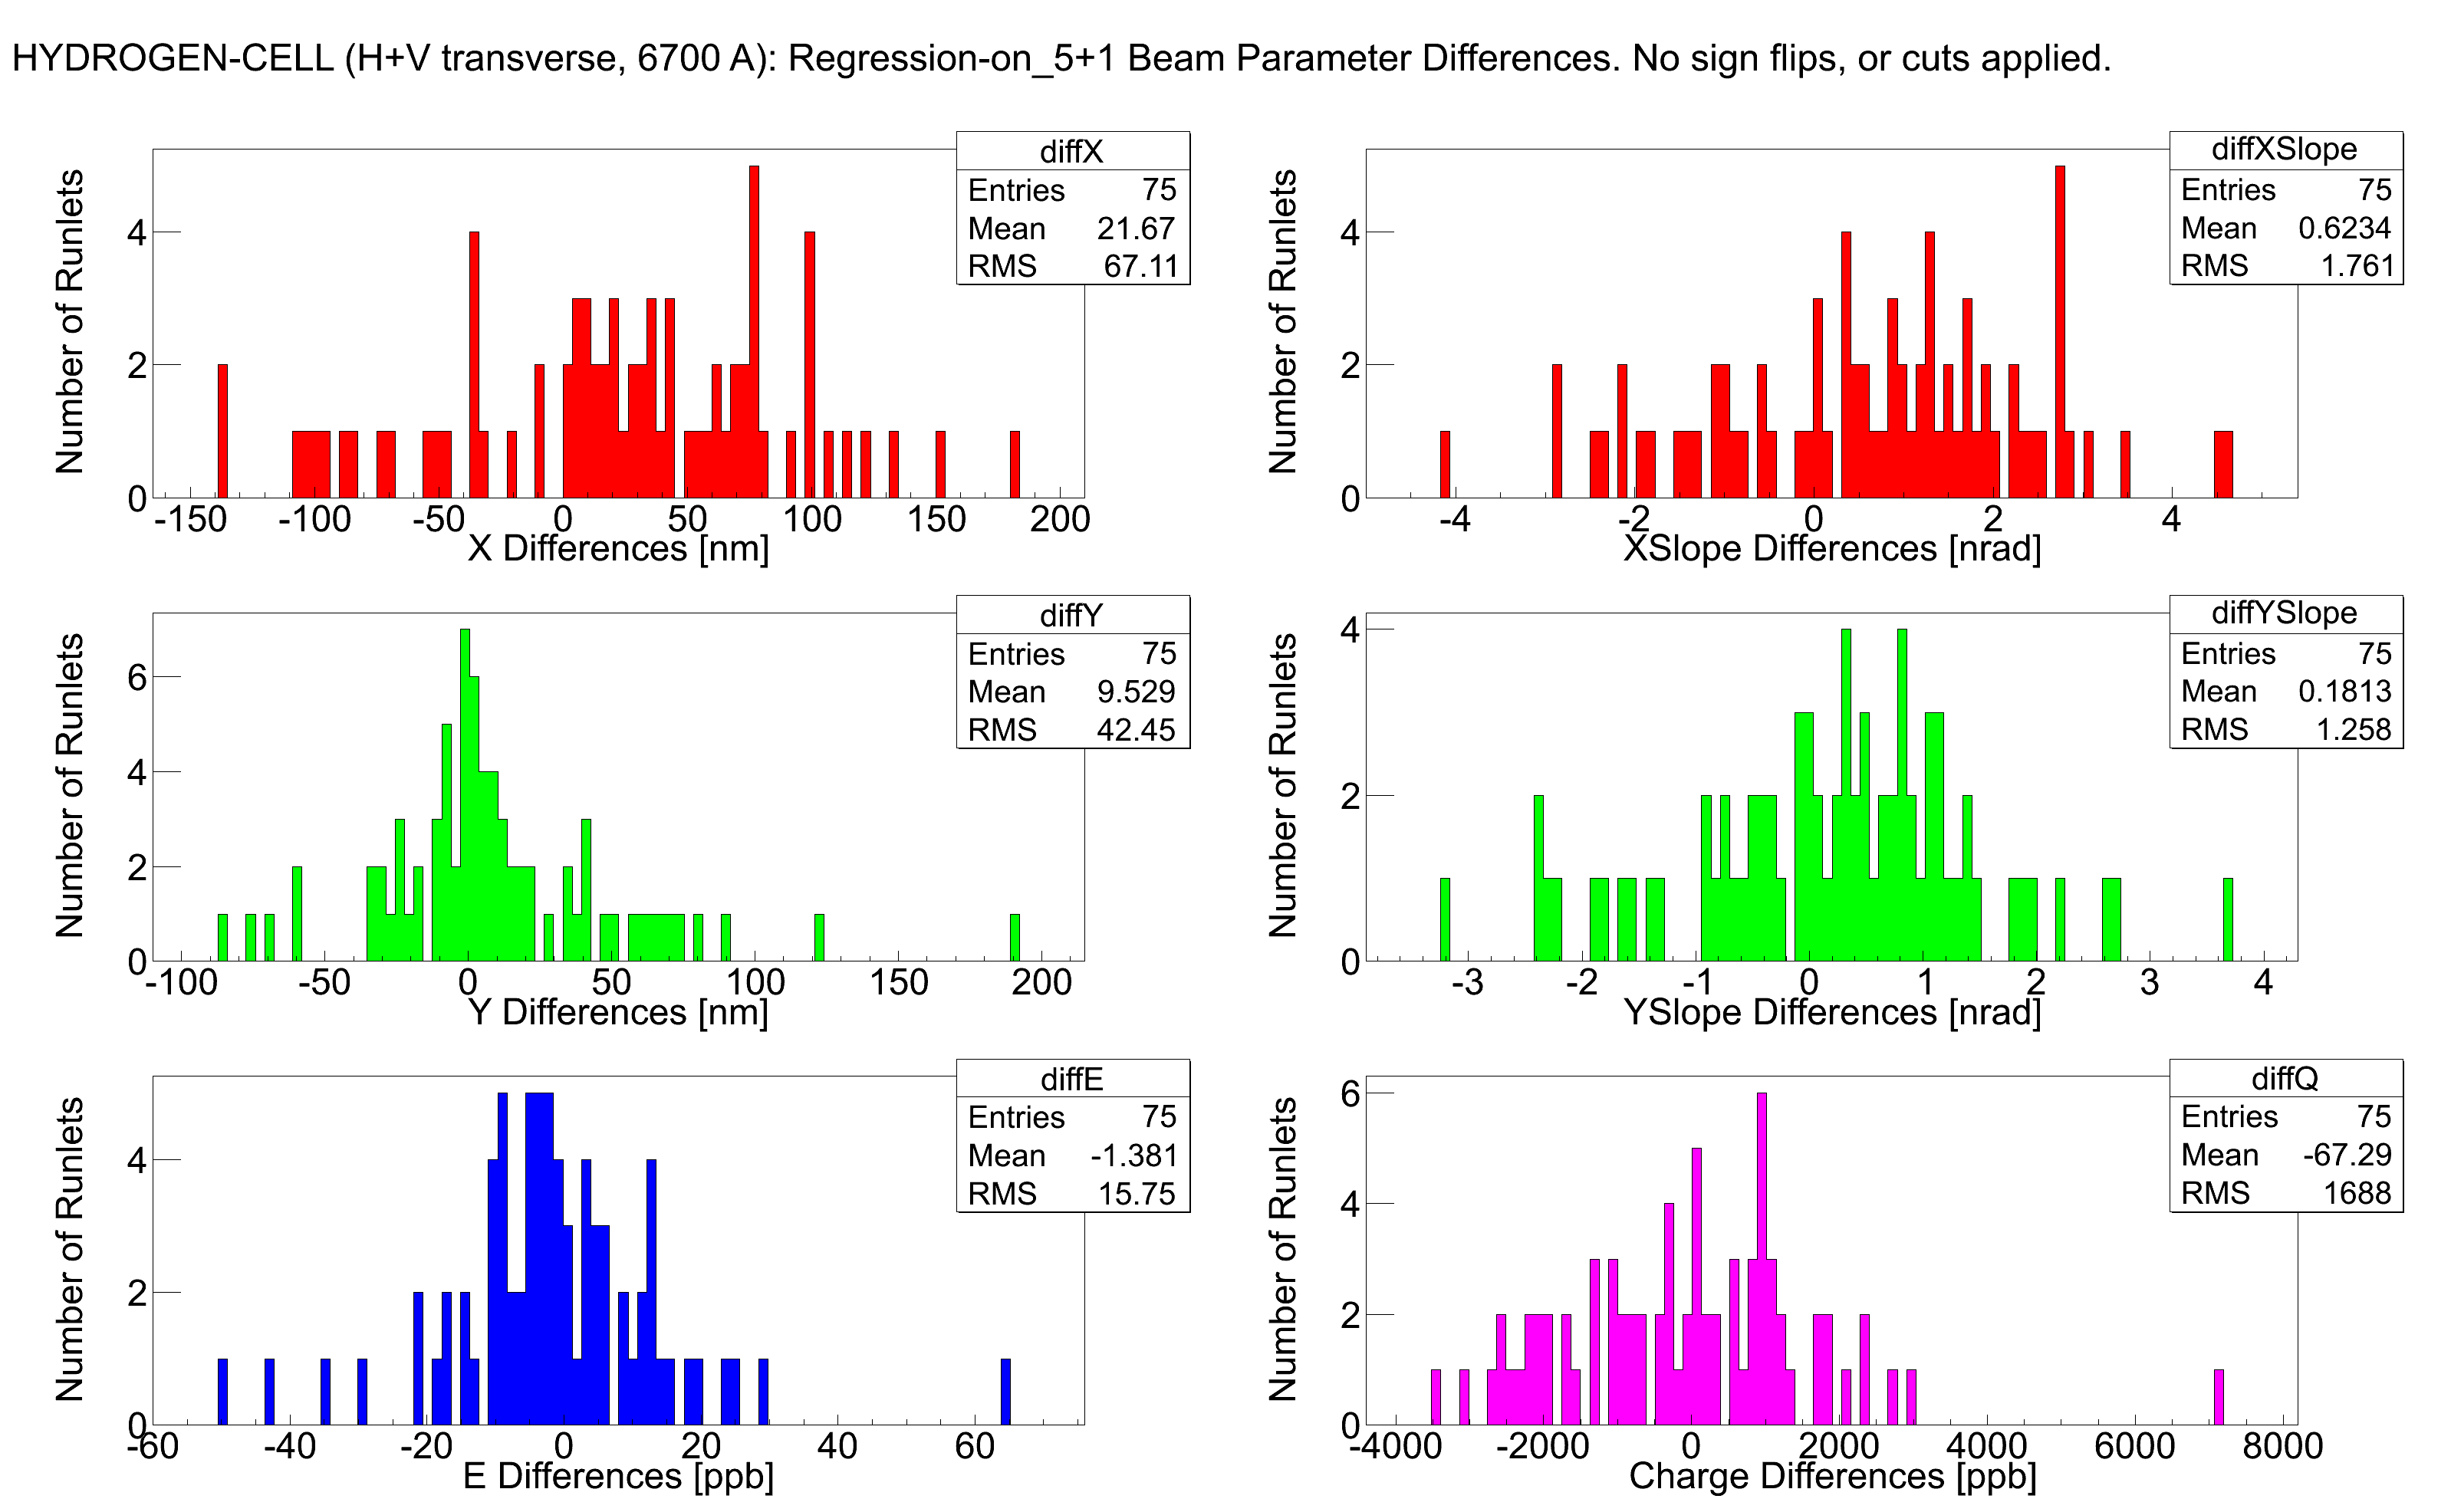
\includegraphics[width=15.0cm]{figures/differences_6700_LH2_off_on_5+1}
	\end{center}
	\caption
%	[Beam parameter differences for the Hydrogen transverse data set.]	
	{Beam parameter differences for the Hydrogen transverse data set.}
	\label{fig:differences_6700_LH2_off_on_5+1}
\end{figure}

\begin{table}[!h]
\begin{center}
  	\caption
%	[Beam parameter differences for the Hydrogen horizontal and vertical transverse data sets.] 
  	{Beam parameter differences for the Hydrogen horizontal and vertical transverse data sets. The X differences are higher compared to Y differences.}
  \begin{tabular}{ c | c  c  c  c }
%	\hline
    \noalign{\hrule height 1pt}
    Beam parameter & \multirow{2}{*}{IHWP IN}	&	\multirow{2}{*}{IHWP OUT} &	 \multirow{2}{*}{($<$IN$>$+$<$OUT$>$)/2}	&	\multirow{2}{*}{($<$IN$>$,-$<$OUT$>$)} \\ 
%	\hline
    	differences &  &  & & \\
%	\hline
    \noalign{\hrule height 1pt}
    \multicolumn{5}{c}{Horizontal Transverse} \\
    \hline
	$\Delta$X~[nm] & 23.8~$\pm$~2.1 & 20.6~$\pm$~2.3 & 22.2~$\pm$~1.6	& 3.6~$\pm$~1.6\\
	$\Delta$Y~[nm]	& 6.9~$\pm$~2.1 & 5.6~$\pm$~2.3 & 6.2~$\pm$~1.6 & 1.2~$\pm$~1.6 \\
	$\Delta$X$^{\prime}$~[nrad] & 0.7~$\pm$~0.1 & 0.7~$\pm$~0.1 & 0.7~$\pm$~0.1	& 0.1~$\pm$~0.1\\
	$\Delta$Y$^{\prime}$~[nrad] & 0.2~$\pm$~0.1 & -0.3~$\pm$~0.1 & -0.0~$\pm$~0.1	& 0.3~$\pm$~0.1\\
	$\Delta$E~[ppb]	& -2.3~$\pm$~2.1 & -1.5~$\pm$~2.3 & -1.9~$\pm$~1.6	& -0.6~$\pm$~1.6\\
	$\Delta$A$_{Q}$~[ppb]	& 8.2~$\pm$~0.5 & -237.3~$\pm$~55.6 & -114.6~$\pm$~27.8	& 8.2~$\pm$~0.5\\
%	\hline
    \noalign{\hrule height 1pt}
    \multicolumn{5}{c}{Vertical Transverse} \\
    \hline
	$\Delta$X~[nm] & 15.4~$\pm$~3.1	& 58.0~$\pm$~3.7 & 36.7~$\pm$~2.4 & -15.2~$\pm$~2.4 \\
	$\Delta$Y~[nm]	& 20.2~$\pm$~3.1 & 15.4~$\pm$~3.6 & 17.8~$\pm$~2.4 & 5.3~$\pm$~2.4 \\
	$\Delta$X$^{\prime}$~[nrad] & 0.6~$\pm$~0.2	& 1.3~$\pm$~0.2 & 1.0~$\pm$~0.1 & -0.2~$\pm$~0.1 \\
	$\Delta$Y$^{\prime}$~[nrad] & 0.6~$\pm$~0.2	& 0.9~$\pm$~0.2 & 0.7~$\pm$~0.1 & -0.0~$\pm$~0.1 \\
	$\Delta$E~[ppb]	& 0.5~$\pm$~3.1	& -5.4~$\pm$~3.6 & -2.4~$\pm$~2.4 & 2.6~$\pm$~2.4 \\
	$\Delta$A$_{Q}$~[ppb]	& 60.1~$\pm$~0.7	& 158.1~$\pm$~88.1 & 109.1~$\pm$~44.1 & 60.1~$\pm$~0.7 \\
    \noalign{\hrule height 1pt}
  	\end{tabular}
  \label{tab:differences}
\end{center}
\end{table}


\begin{figure}[!h]
	\begin{center}
	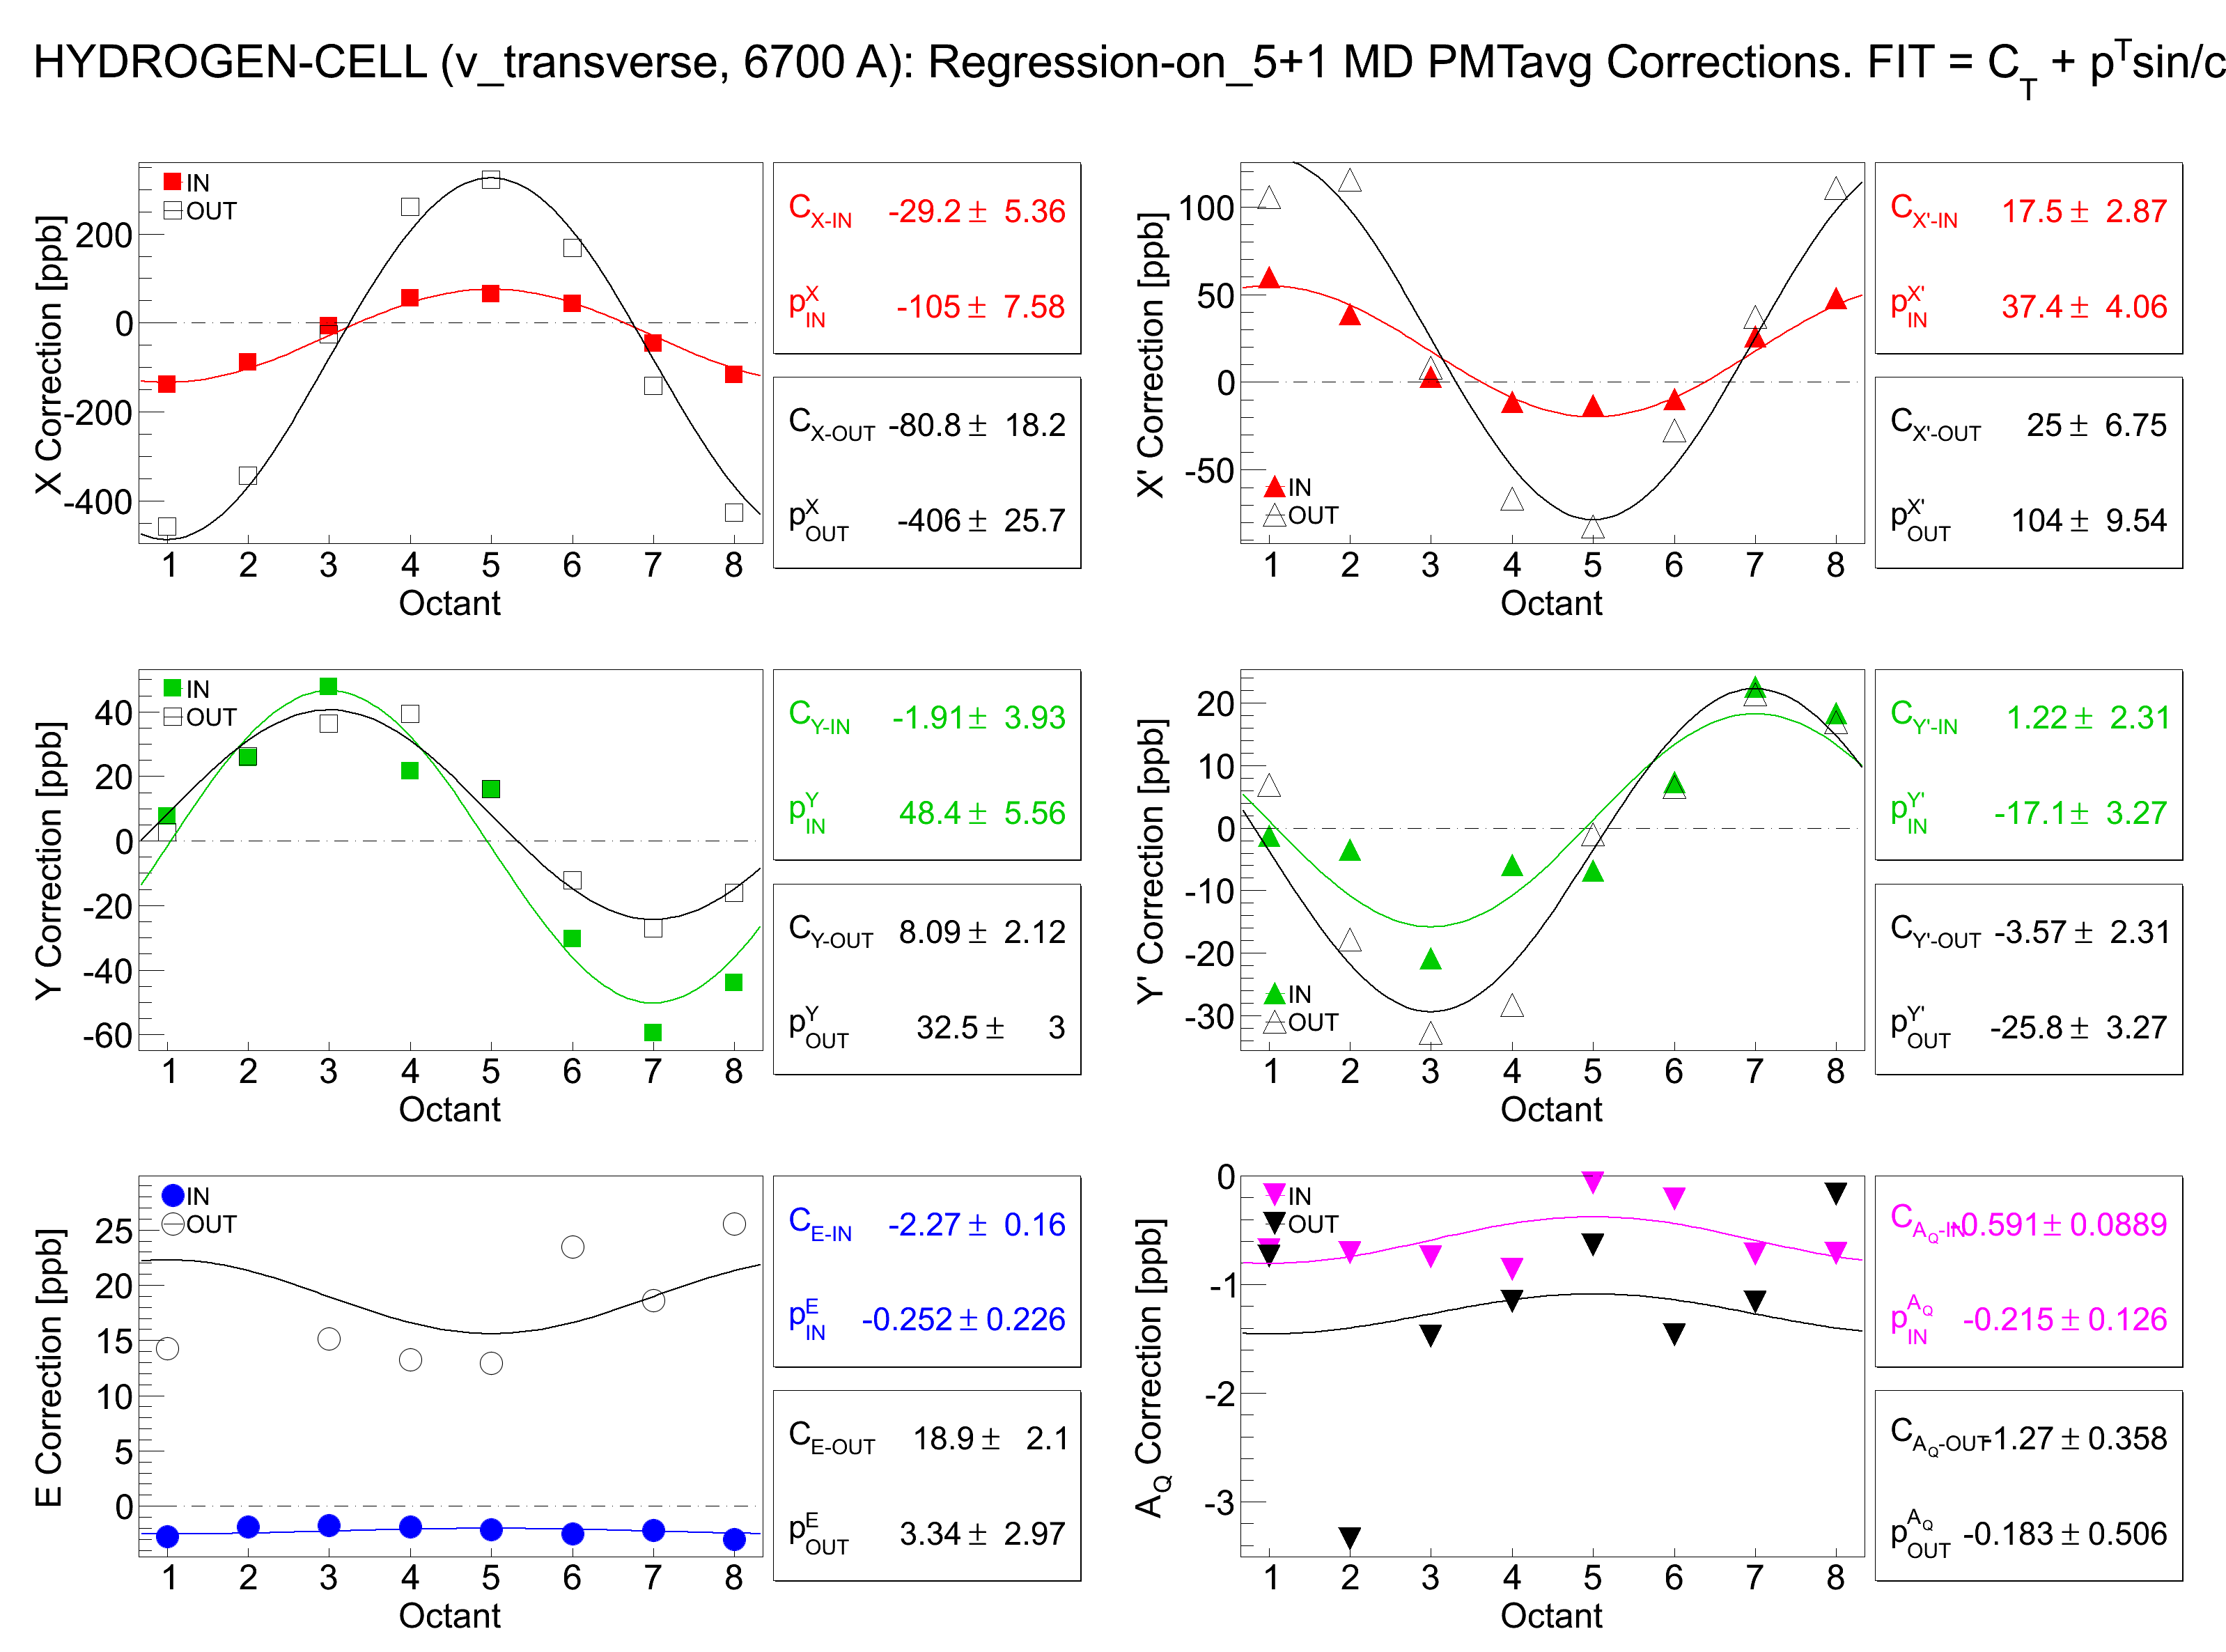
\includegraphics[width=15.0cm]{figures/MD_v_transverse_5+1_corrections}
	\end{center}
	\caption
%	[Main detector corrections vs octant for vertical transverse data set.]	
	{Main detector corrections (using sensitivities from ``5+1" regression scheme) vs octant for vertical LH$_{2}$ transverse data set are shown here. Beam positions and angles have sinusoidal dependence with octant inherited from the sensitivities. No such dependence is seen for energy and charge. Both IHWP states are shown separately for each beam parameter.}
	\label{fig:MD_v_transverse_5+1_corrections}
\end{figure}

\begin{figure}[!h]
	\begin{center}
	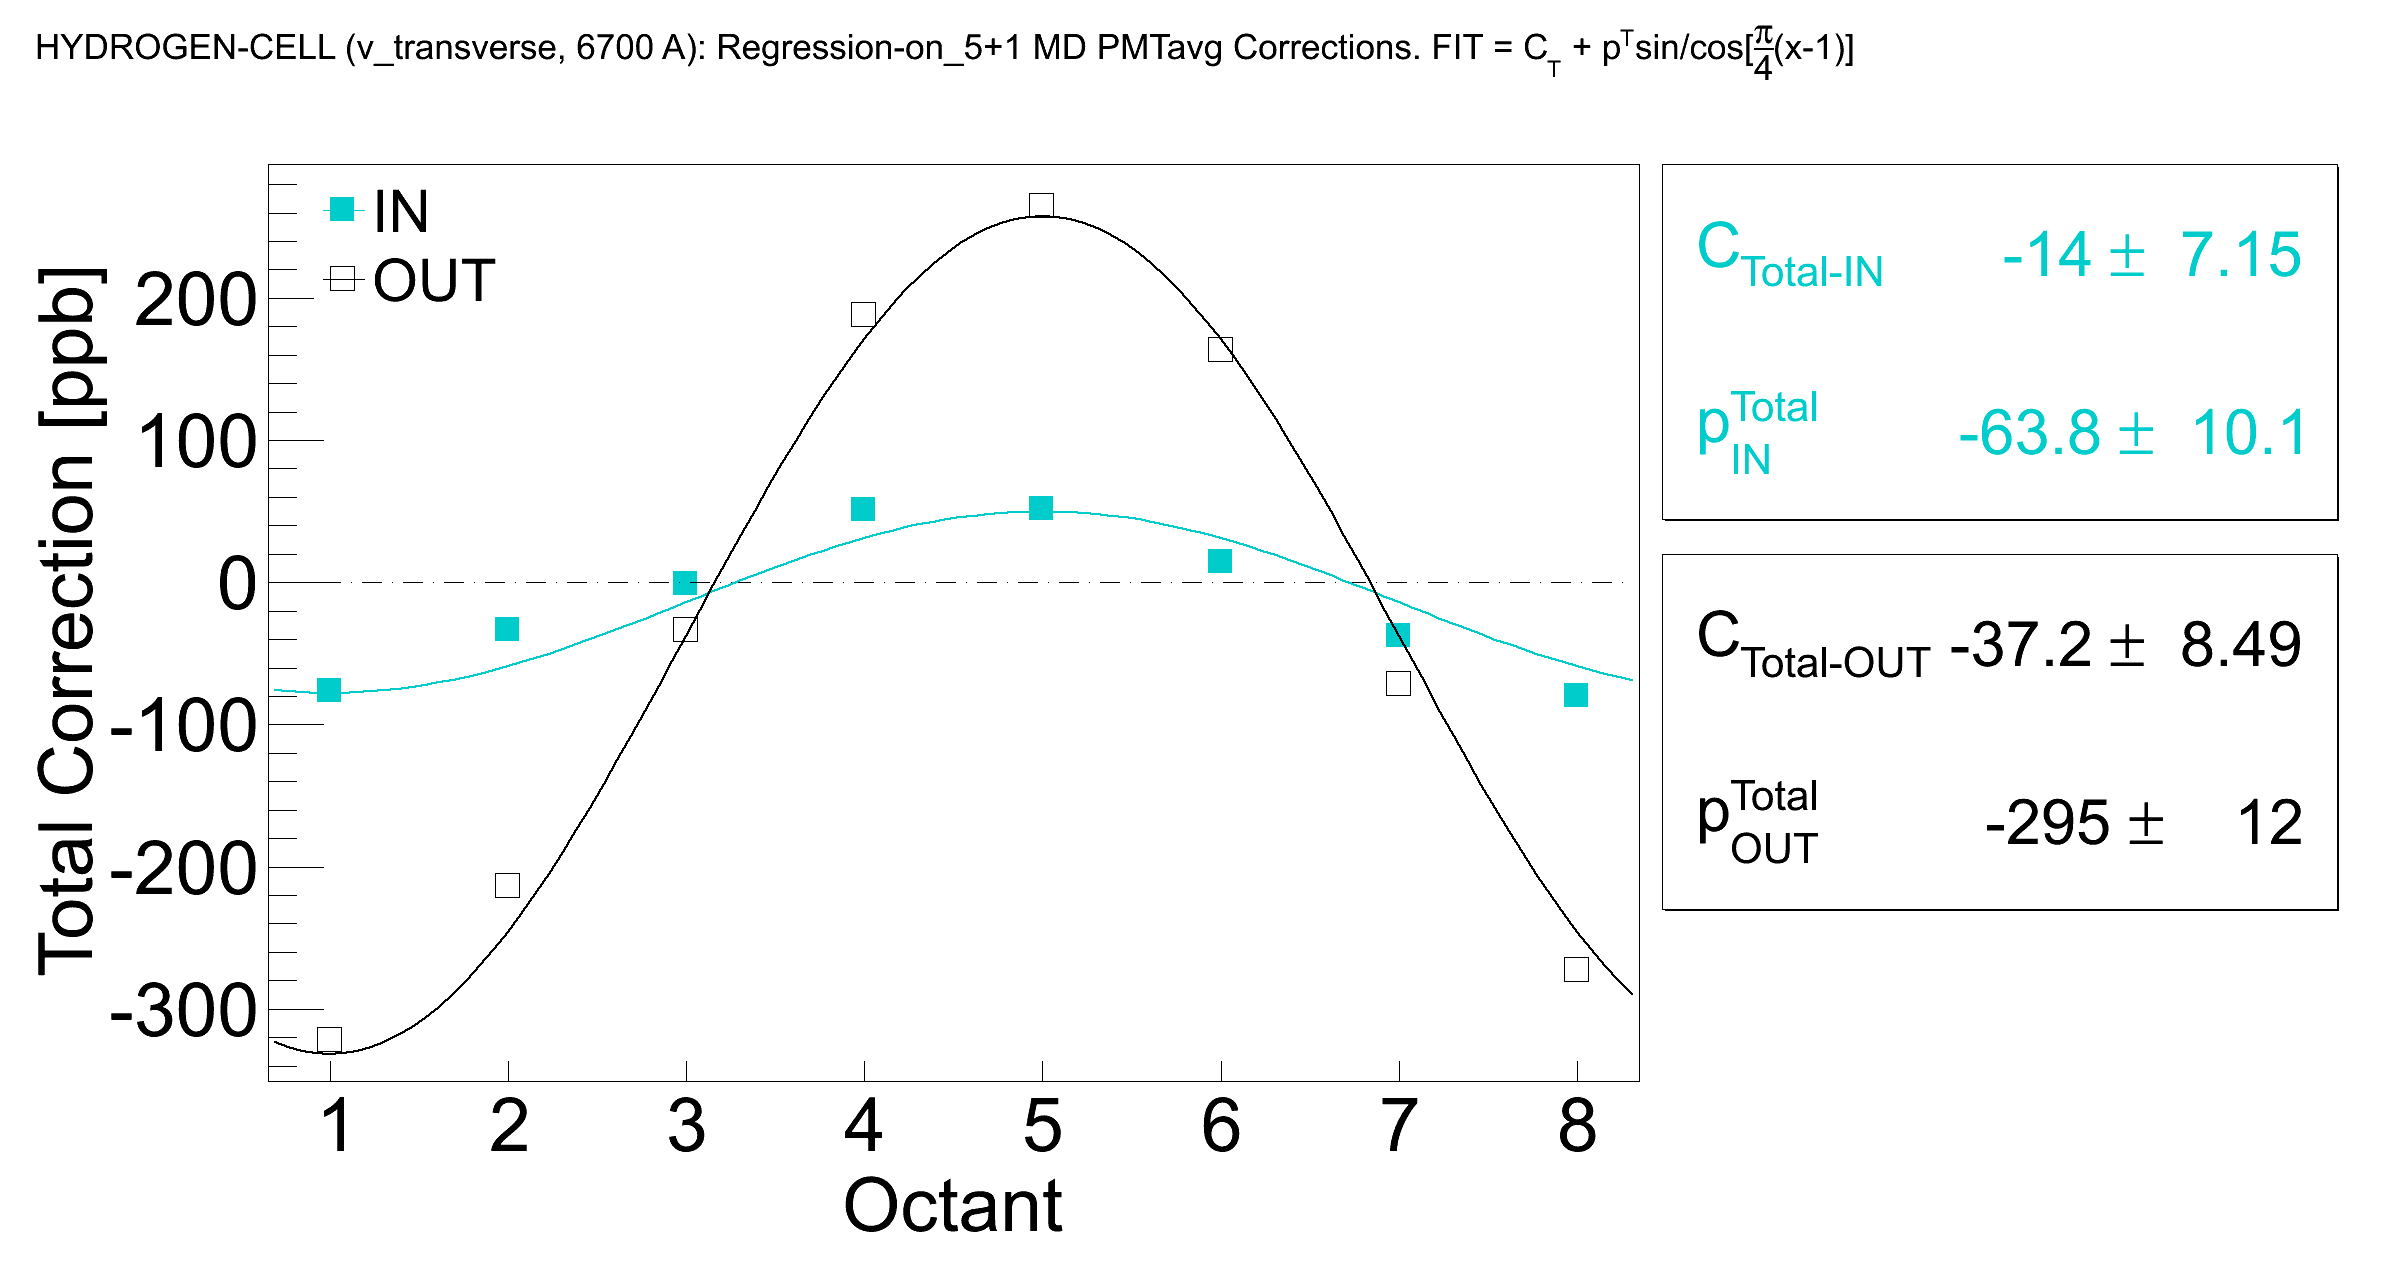
\includegraphics[width=10.0cm]{figures/MD_v_transverse_5+1_TotalCorrections}
	\end{center}
	\caption
%	[Total corrections vs octant for vertical transverse data set.]	
	{Total corrections in ``5+1" regression scheme vs octant for vertical LH$_{2}$ transverse data set are shown here. The total correction is the sum of all the corrections (with sign) shown in Figure~\ref{fig:MD_v_transverse_5+1_corrections}.}
	\label{fig:MD_v_transverse_5+1_TotalCorrections}
\end{figure}

\begin{figure}[!h]
	\begin{center}
	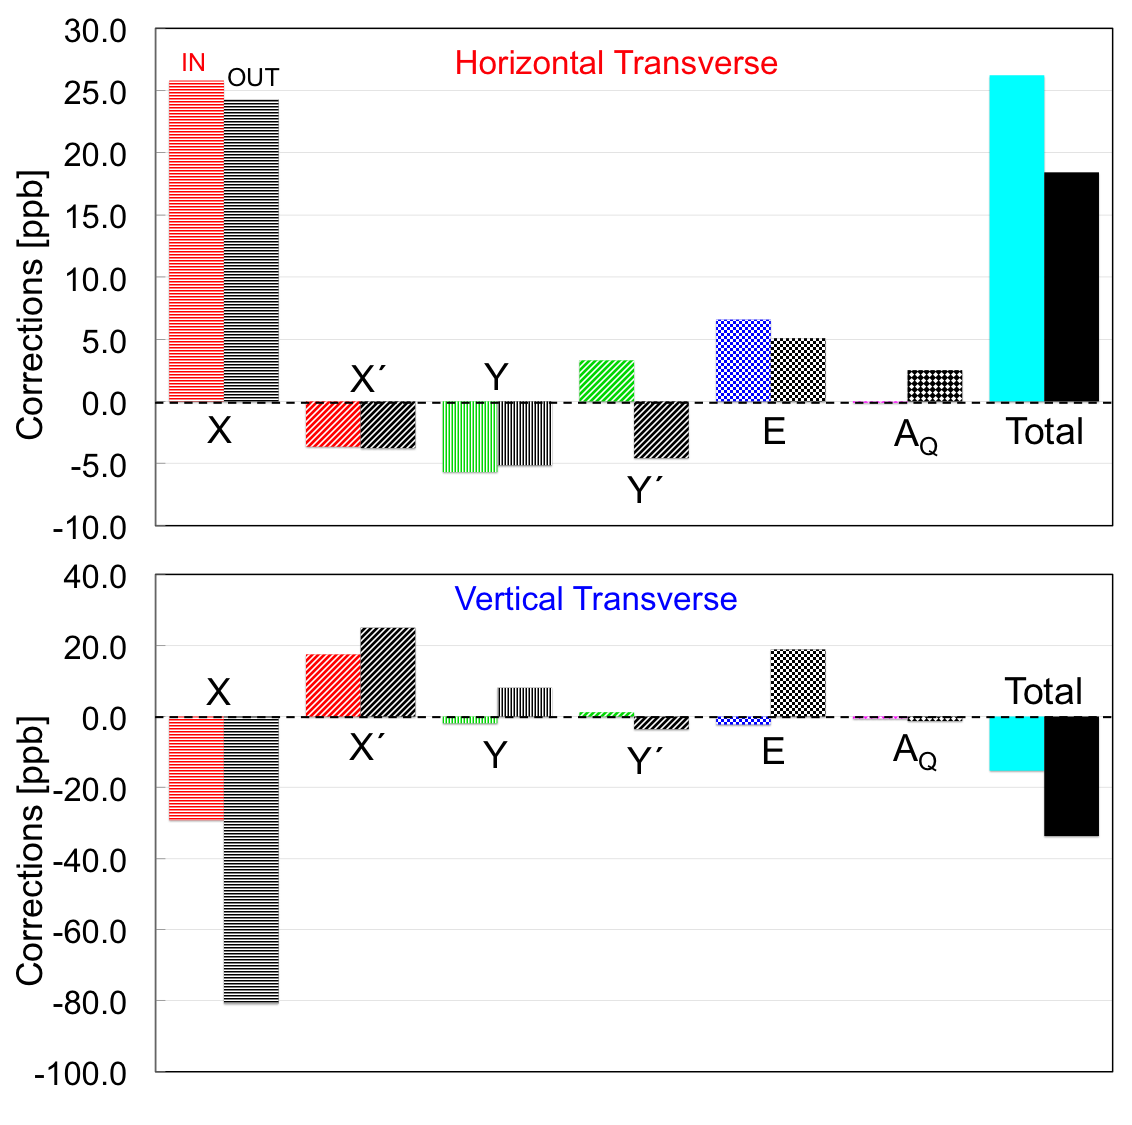
\includegraphics[width=15.0cm]{figures/correctionSummary_LH2}
	\end{center}
	\caption
%	[Main detector corrections for horizontal and vertical LH$_{2}$ transverse data sets are shown here.]	
	{Main detector corrections (using sensitivities from ``5+1" regression scheme) for horizontal (top) and vertical (bottom) LH$_{2}$ transverse data sets are shown here. Both IHWP states are shown separately for each beam parameter. The total correction is the sum of all the corrections (with sign).}
	\label{fig:correctionSummary_LH2}
\end{figure}


%\begin{table}[!h]
%\begin{center}
%  	\caption
%	[Beam parameter differences during for the horizontal and vertical transverse data set.]  	
%  	{Beam parameter differences during for the horizontal and vertical transverse data set.}
%  \begin{tabular}{ c | c  c | c  c }
%%	\hline
%    \noalign{\hrule height 1pt}
%         \multirow{2}{*}{Beam parameter} & \multicolumn{2}{c|}{Horizontal} & \multicolumn{2}{c}{Vertical} \\ 
%     \cline{2-5}
%%	\hline
%    	&	IHWP IN	&	IHWP OUT &	 IHWP IN	&	IHWP OUT  \\
%%	\hline
%    \noalign{\hrule height 1pt}
%	Target X position differences $\Delta$X~[nm] & 23.8~$\pm$~2.1 & 20.6~$\pm$~2.3 & 15.4~$\pm$~3.1	& 58.0~$\pm$~3.6\\
%	Target Y position differences $\Delta$Y~[nm]	& 6.9~$\pm$~2.1 & 5.6~$\pm$~2.3 & 20.2~$\pm$~3.1 & 15.4~$\pm$~3.6 \\
%	Target X angle differences $\Delta$X$^{\prime}$~[nrad] & 0.7~$\pm$~0.1 & 0.7~$\pm$~0.1 & 0.6~$\pm$~0.2	& 1.3~$\pm$~0.2\\
%	Target Y angle differences $\Delta$Y$^{\prime}$~[nrad] & 0.2~$\pm$~0.1 & -0.3~$\pm$~0.1 & 0.6~$\pm$~0.2	& 0.9~$\pm$~0.2\\
%	Energy differences $\Delta$E~[ppb]	& -2.3~$\pm$~2.1 & -1.5~$\pm$~2.3 & 0.5~$\pm$~3.1	& -5.4~$\pm$~3.6\\
%	Charge asymmetry $\Delta$A$_{Q}$~[ppb]	& 8.2~$\pm$~0.5 & -237.3~$\pm$~55.6 & 60.1~$\pm$~0.7	& 158.1~$\pm$~88.1\\
%%	\hline
%    \noalign{\hrule height 1pt}
%  	\end{tabular}
%  \label{tab:differences}
%\end{center}
%\end{table}

\begin{figure}[!h]
	\begin{center}
	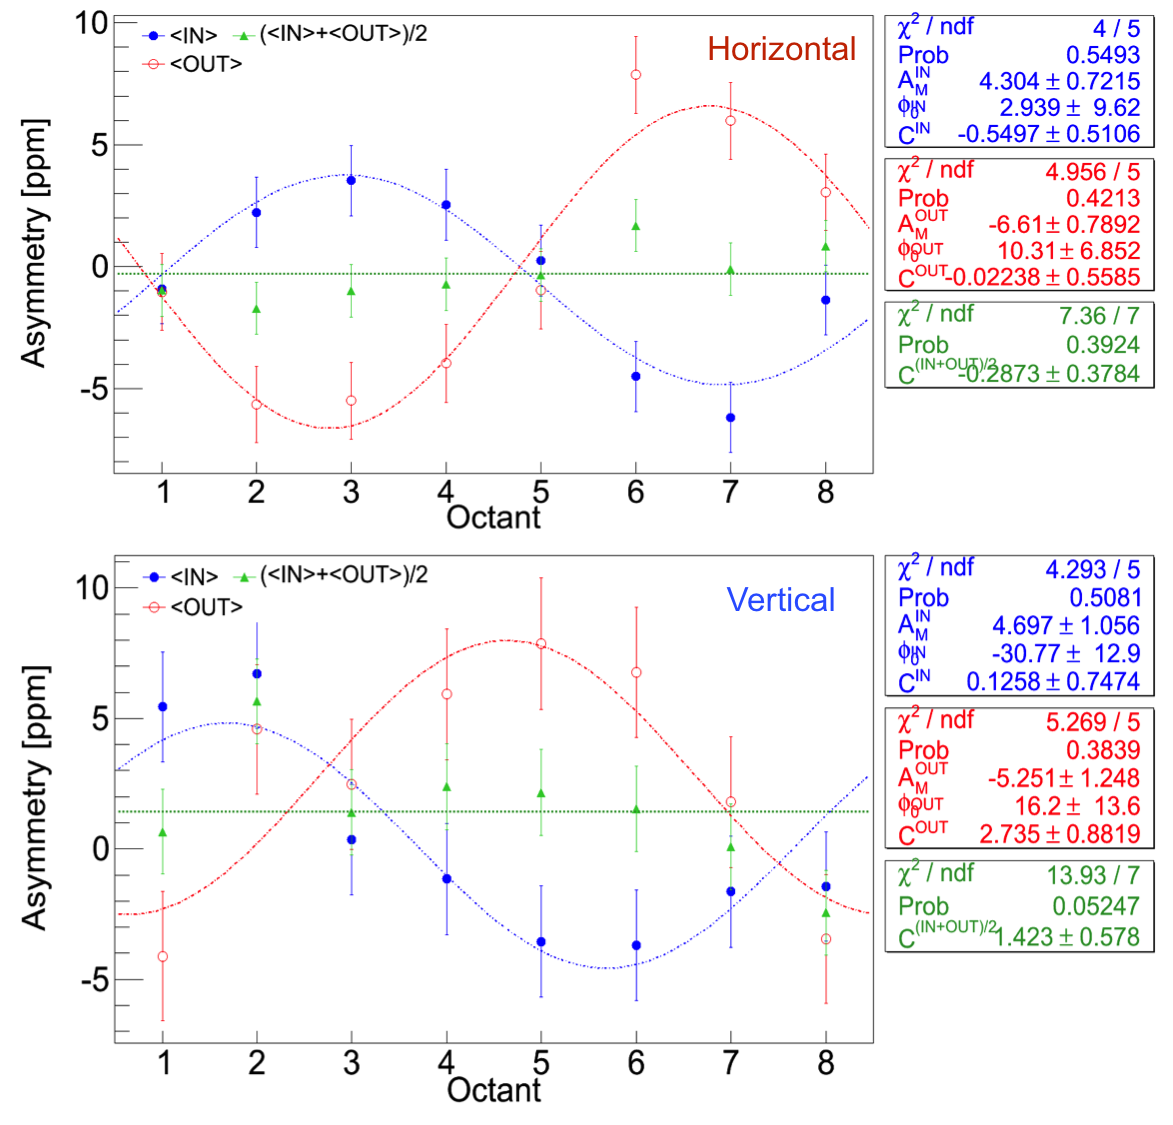
\includegraphics[width=15.0cm]{figures/asymmetry_In_Out_H2}
	\end{center}
	\caption
%	[Main detector asymmetry for horizontal, vertical data set.]
	{Main detector asymmetry for horizontal (top), vertical (bottom) data set. For comparison, asymmetries for IN and OUT data are also shown separately. The regressed asymmetries change sign with the insertion of the IHWP with comparable amplitudes. The ($<$IN$>$+$<$OUT$>$)/2 asymmetries of the eight \v{C}erenkov detectors, given by $C^{\rm (IN+OUT)/2}$ is compatible with zero except in the vertical data set. The extraction of BNSSA depends on the amplitudes in the fits and by comparison of IN and OUT, not the constant term.}
	\label{fig:asymmetry_In_Out_H2}
\end{figure}

The regressed ``5+1" asymmetries measured using horizontal and vertical transverse polarization beam on LH$_{2}$ target are shown in Figure~\ref{fig:asymmetry_In_Out_H2}. The azimuthal modulating asymmetry flips sign with the insertion of the IHWP as expected. The vertical asymmetry fits may show sign of phase shift between IHWP IN and IHWP OUT settings, but may be explained due to statistical fluctuation. Transverse polarization angle was $\sim$2-3\degrees{} off from ideal settings during the measurement~\cite{elogAcc:riad_1567146, hclog:page_219054}, which can not be confirmed with the statistics in hand. The null asymmetry ($<$IN$>$+$<$OUT$>$)/2 given by the $C^{\rm (IN+OUT)/2}$ are compatible with zero  within the measurement uncertainties. This indicates the azimuthal modulating signal in both IHWP IN and OUT are the same, and the non-polarization dependent false beam asymmetries were successfully removed by the regression.

The error weighted value of IN-OUT yields the measured regressed asymmetry for each bar. As expected from the azimuthal dependence of the BNSSA, there is a 90\degrees{} phase offset between horizontal and vertical, as shown in Figure~\ref{fig:asymmetry_H2}. The measured five-parameter\footnote{The charge asymmetry was not included as regression parameter in the final asymmetry calculation, as it is not an helicity correlated beam property (more details in section~\ref{Regression Scheme Dependence}).} regressed asymmetries using horizontal and vertical transverse polarization are extracted as $\epsilon_{M}^{H}$ = 5.343~$\pm$~0.532~ppm and  $\epsilon_{M}^{V}$ = 4.525~$\pm$~0.806~ppm, respectively. The combined (error weighted average) regressed asymmetry from horizontal and vertical transverse polarization is given by

\begin{equation} \label{equ:asymmetryMeasured}
\epsilon_{M} = 5.047~\pm~0.444~\text{ppm (stat)}.
\end{equation}

This measurement provides a $\sim$9\% statistical measurement of the BNSSA in inelastic e+p scattering (not corrected for backgrounds, polarization or other experimental related systematic uncertainties). Regression has small effect on the extracted measured asymmetries ($\lesssim$4\%).

\begin{figure}[!h]
	\begin{center}
	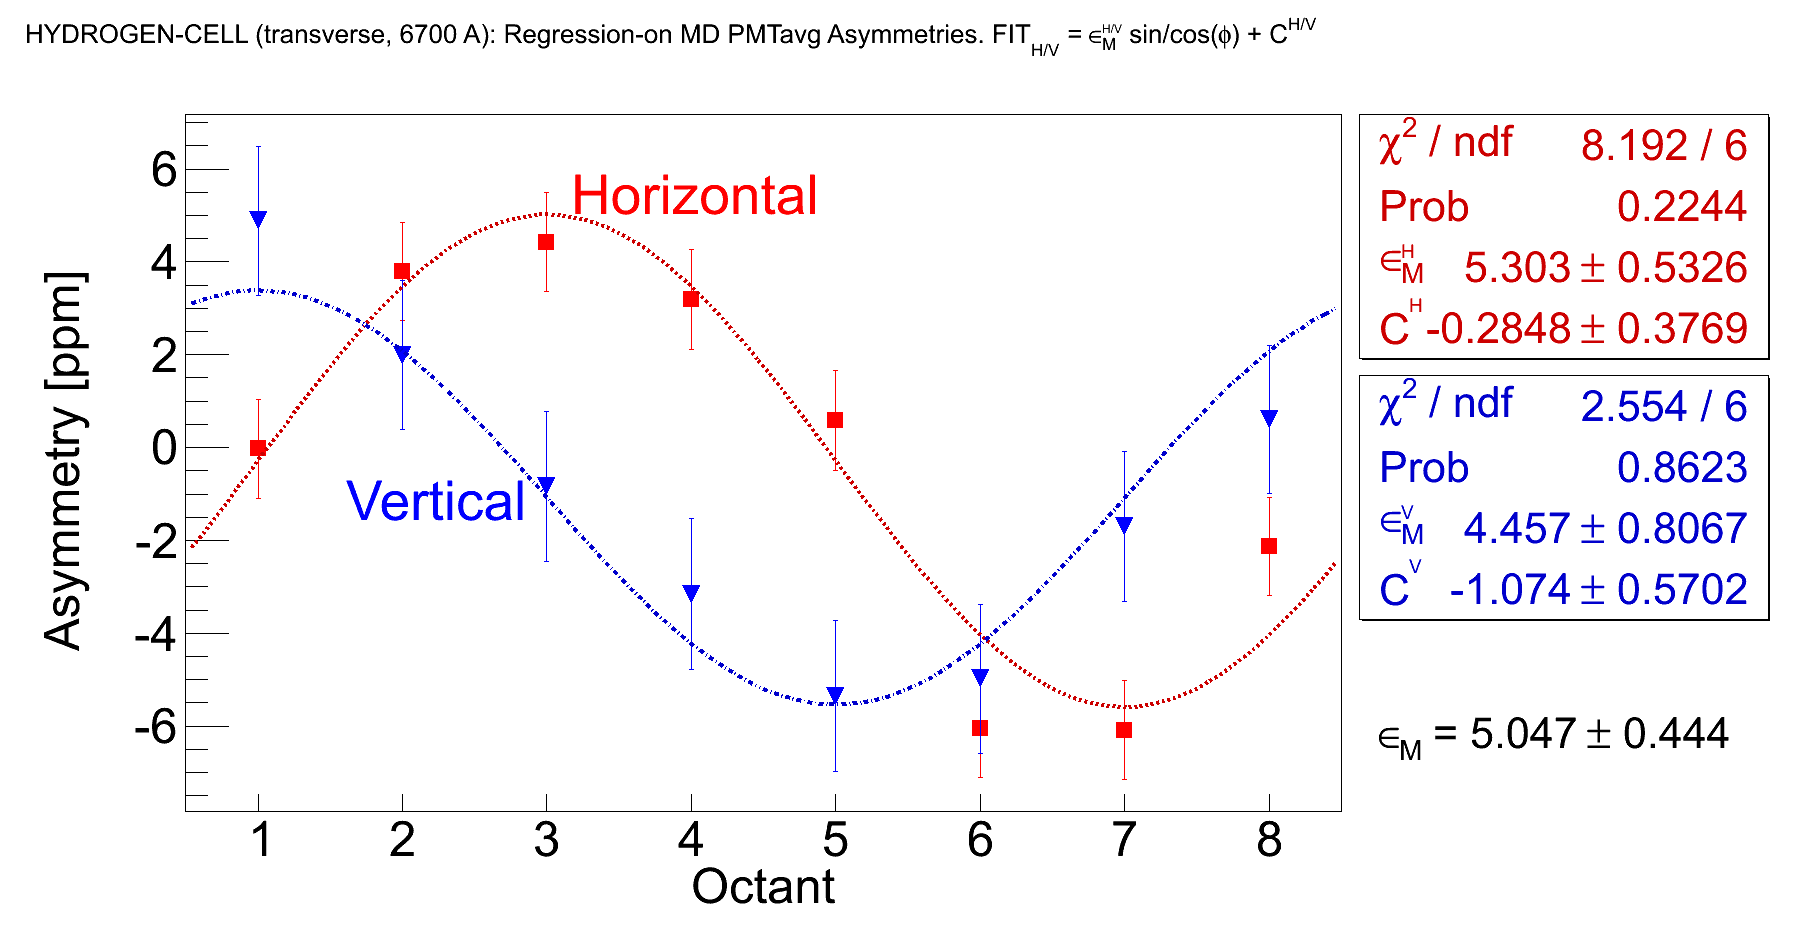
\includegraphics[width=15.0cm]{figures/asymmetry_H2}
	\end{center}
	\caption
%	[Regressed main detector asymmetry for horizontal, vertical transverse data set on LH$_{2}$.]	
	{Regressed main detector asymmetry for horizontal, vertical transverse polarization are shown with red circle and blue square, respectively. Data points for horizontal transverse are $\sim$4~hour long measurement, whereas vertical transverse data points are $\sim$2~hour long. The fit functions used are $\epsilon_{M}^{H} \sin(\phi + \phi_{0}^{H}) + C^{H}$ for horizontal transverse and $\epsilon_{M}^{V} \cos(\phi + \phi_{0}^{V}) + C^{V}$ for vertical transverse, respectively. Asymmetries in each case shows $\sim$90\degrees{} phase offset, as expected between horizontal and vertical configurations.}
	\label{fig:asymmetry_H2}
\end{figure}

%\subsection{Azimuthal Acceptance Correction}
%\label{Azimuthal Acceptance Correction}
%
%The acceptance of a single Q-weak \v{C}erenkov detector is only 49\% of an octant (section~\ref{Q-weak Kinematics}), so the reported asymmetry from a detector is an average over 22\degrees{} azimuthal angle ($\phi$). Each detector bar measures an average asymmetry over a range of $\phi$ selected by the collimators (details in~\cite{buddhini_qweak, elog:birchall_analysis373}). The effect of averaging cosines for a variable of the form $y(\phi) = \epsilon\cos(\phi + \delta)$ over the azimuthal angle yields 
%
%\begin{equation} \label{equ:eqDetectorNonlinearity}
%AVG[y(\phi)] = \frac{ \epsilon\int_{\phi_{0}-\Delta\phi}^{\phi_{0}+\Delta\phi} \cos(\phi+\delta)\,\mathrm{d}\phi }{(\phi_{0}+\Delta\phi)-(\phi_{0}-\Delta\phi)} = \epsilon\cos (\phi_{0} + \delta) \times \frac{\sin\Delta\phi}{\Delta\phi}, 
%\end{equation}
%
%\noindent
%where $\phi_{0}$ is the nominal azimuthal location of the detector with $\Delta\phi$ coverage. Similarly, for sines, $AVG[y(\phi)] = \epsilon\sin (\phi_{0} + \delta) \times \frac{\sin\Delta\phi}{\Delta\phi}$. So the measured asymmetry from each detector needs to be scaled by a factor of $\frac{\sin\Delta\phi}{\Delta\phi}$ to correct for the acceptance\footnote{Here, the collimator is assumed to remove 49\% of the octant acceptance (i.e 49\% of 45\degrees{})}. $\Delta\phi$ = 11.025\degrees{} yields the scale factor to be $\frac{\sin\Delta\phi}{\Delta\phi}$ = 0.9938.
%% implies the amplitude from the transverse fits to the octant asymmetries should be scaled by a factor of $\frac{\sin\Delta\phi}{\Delta\phi}$ = 0.9938. 
%The detector acceptance corrected measured asymmetry can be extracted as
%
%\begin{equation} \label{equ:asymmetryDetAcptCorrected}
%\epsilon_{M}^{\rm in} = \frac{\epsilon_{M}}{0.9938} = 5.127~\text{ppm}.
%\end{equation}
%
%A conservative 50\% uncertainty was used for $\Delta\phi$, which yields a systematic uncertainty of 0.004 in the correction.

%%%%%%%%%%%%%%%%%%%%%%%%%%%%%%%%%%%%%%%%%%%%%%%%%%%%%%%%%%%%%
\section{Systematic Uncertainties}
\label{Systematic Uncertainties}
The dominant uncertainty in the measured asymmetry for this measurement is statistical (9\%). A preliminary treatment of the systematic uncertainty performed on the data set is presented in this section.

\begin{table}[!h]
 \begin{center}
	\caption
%	[Asymmetries from different regression schemes for horizontal and vertical transverse data set.]
	{Asymmetries from different regression schemes, along with the raw asymmetry, are shown for horizontal and vertical transverse data sets from Run 2 Pass 5 database. Corrections are small ($\lesssim$4\%) compared to the amplitude of the measured asymmetry. The schemes without and with charge as regression variable are shown separately. Set 5 and 6 were not available due to failure of BPM 9b during Run 2. Set 9 was ignored for this analysis as it used the upstream luminosity monitor as an independent variable (more details about regression variables are in APPENDIX~\ref{REGRESSION SCHEMES}).}
  \begin{tabular}{ c | c  c | c  c}
%    \hline
    \noalign{\hrule height 1pt}
     \multirow{2}{*}{Regression} & \multicolumn{2}{c|}{Horizontal} & \multicolumn{2}{c}{Vertical} \\ 
     \cline{2-5}
     \multirow{2}{*}{scheme} & Asymmetry & Correction & Asymmetry & Correction\\
	& [ppm]  & [ppm] & [ppm]  & [ppm] \\
%	\hline
    \noalign{\hrule height 1pt}
	UnReg	&	5.339	&	0.000	& 4.602	&	0.000	\\ \hline
	std		&	5.343	&	0.004	& 4.524	&	-0.078	\\
	set7		&	5.347	&	0.007	& 4.529	&	-0.073	\\
	set11	&	5.343	&	0.004	& 4.524	&	-0.078	\\ \hline
	5+1		&	5.343	&	0.004	& 4.525	&	-0.077	\\
	set3		&	5.343	&	0.004	& 4.525	&	-0.077	\\
	set4		&	5.343	&	0.004	& 4.527	&	-0.076	\\
	set8		&	5.346	&	0.007	& 4.531	&	-0.072	\\
\st{set9}	&	\st{5.343}	&	\st{0.003}	& \st{4.534}	&	\st{-0.069}	\\
	set10	&	5.343	&	0.003	& 4.526	&	-0.077	\\
%	\hline
    \noalign{\hrule height 1pt}
	Max - Min	&	set8 - set10 & 0.004	& set8 - set11	&	0.006	\\		
%	\hline
    \noalign{\hrule height 1pt}
   \end{tabular}
 \label{tab:regression_scheme_dependence}
 \end{center}
\end{table}

\subsection{Regression Scheme Dependence}
\label{Regression Scheme Dependence}

Since the five-parameter (``std") linear regression scheme used for this analysis is only one of the many different schemes available, it was worth investigating the scheme dependence. A list of all the independent variables for different regression sets are shown in APPENDIX~\ref{REGRESSION SCHEMES}. Ideally, the regression corrections from all the schemes should agree if all equipment is functioning properly and the regression is being done properly. Small differences in the corrections can arise from differences in the noise, resolution, and non-linear response of the monitors. To compare for the systematic studies, a common set of event cuts~\cite{rakitha_qweak} are applied to all regression schemes to match the quartets used by each scheme.
The results are summarized in Table~\ref{tab:regression_scheme_dependence}. The regression scheme dependence uncertainty is defined as the largest difference between all of the schemes and estimated to be 0.004~ppm for horizontal transverse and 0.006~ppm for vertical transverse data set.

%\begin{center}
%\framebox[\frameboxsize][c]{Systematic error due to regression schemes dependence is $\sim$ 0.0046 ppm.}
%\end{center}

%\newpage
\subsection{Regression Time Dependence}
\label{Regression Time Dependence}

The standard regression algorithm works with 5 minute runlet averaged quantities. The detector sensitivities are averaged over each runlet and corresponding differences are used to correct for the false asymmetry for each quartet in the runlet. There is another systematic uncertainty associated with regression time period that is considered.
%The average sensitivities for a beam parameter with its corresponding differences for a runlet was used to obtain the correction for the beam parameter of a runlet. The regressed asymmetries were then extracted for each runlet using total correction. 
The effect of using slug, few hours ($\sim$2), as time period for the regression instead of runlets was determined. 
The MD error weighted average sensitivities for a slug were calculated and average beam parameter differences for that slug were used to get the corrections, as shown in Equation~\ref{equ:eqCorrection2}. These slug averaged corrections were then used to regress asymmetries (Equation~\ref{equ:eqCorrection1}). 
%Run vs Runlet Correction: 
%The effect of using runlets instead of slug for regression on the extracted transverse spin asymmetry
%was determined by first calculating the error weighted average sensitivities from the elastic
%LH$_{2}$ data set with horizontal transverse polarization and then by using the average beam parameter differences
%on that period to calculate the corrections by hand and by applying them to the unregressed
%asymmetries.

\begin{equation} \label{equ:eqCorrection1}
\langle \epsilon_{\rm reg}\rangle_{\rm slug} = \langle \epsilon_{\rm UnReg}\rangle_{\rm slug} - \langle C\rangle_{\rm slug}
\end{equation}

\begin{equation} \label{equ:eqCorrection2}
\langle C\rangle_{\rm slug} = \sum^{6}_{i=1} \left\langle \frac{\partial\epsilon }{\partial T_{i}}\right\rangle_{\rm slug} \langle\Delta T_{i}\rangle_{\rm slug}
\end{equation}

where $T_{i}$'s are $X$, $X^{\prime}$, $Y$, $X^{\prime}$, $A_{E}$, and  $A_{Q}$. The slug averaged sensitivities and beam parameter differences for the data set are shown in Figure~\ref{fig:MD_v_transverse_5+1_Sensitivities} (also Figure~\ref{fig:MD_h_transverse_5+1_Sensitivities} for horizontal transverse) and Table~\ref{tab:differences}, respectively.
%The impact on regression for using a different time period for averaging sensitivities and differences for horizontal and vertical transverse data set are 0.006~ppm and 0.008~ppm respectively and assigned as regression time dependence systematic uncertainties. More details in APPENDIX-\ref{Beam Normal Single Spin Asymmetry in Inelastic e-p Scattering} section~\ref{Regression Time Dependence 2}.
The impact on regressed asymmetries due to change in the regression averaging time period for horizontal and vertical transverse data set are 0.006~ppm and 0.008~ppm, respectively and are assigned as regression time dependence systematic uncertainties. More details in APPENDIX-\ref{Beam Normal Single Spin Asymmetry in Inelastic e-p Scattering} section~\ref{Regression Time Dependence 2}.

%\begin{table}[!h]
%\begin{center}
%  \begin{tabular}{ c  c  c  c }
%    \hline
%    Asymmetries 		&	Barsum		&	PMTavg	&	Difference	\\
%    			 		&	[ppm]		&	[ppm]	&	[ppm]	\\
%	\hline
%	A$_{M}^{H}$ & 5.34291 &	5.34293 &	0.00002 \\
%	A$_{M}^{V}$ & 4.52568 &	4.52522 &	0.00046 \\
%    \hline
%  	\end{tabular}
%  	\caption[Barsum and PMTavg asymmetries.]{Barsum and PMTavg asymmetries.}
%  \label{tab:BarsumPMTavgAsymmetries}
%\end{center}
%\end{table}
%
%\begin{center}
%\framebox[\frameboxsize][c]{Run vs Runlet correction is $\sim$0.0066~ppm.}
%\end{center}

\begin{figure}[!h]
	\begin{center}
	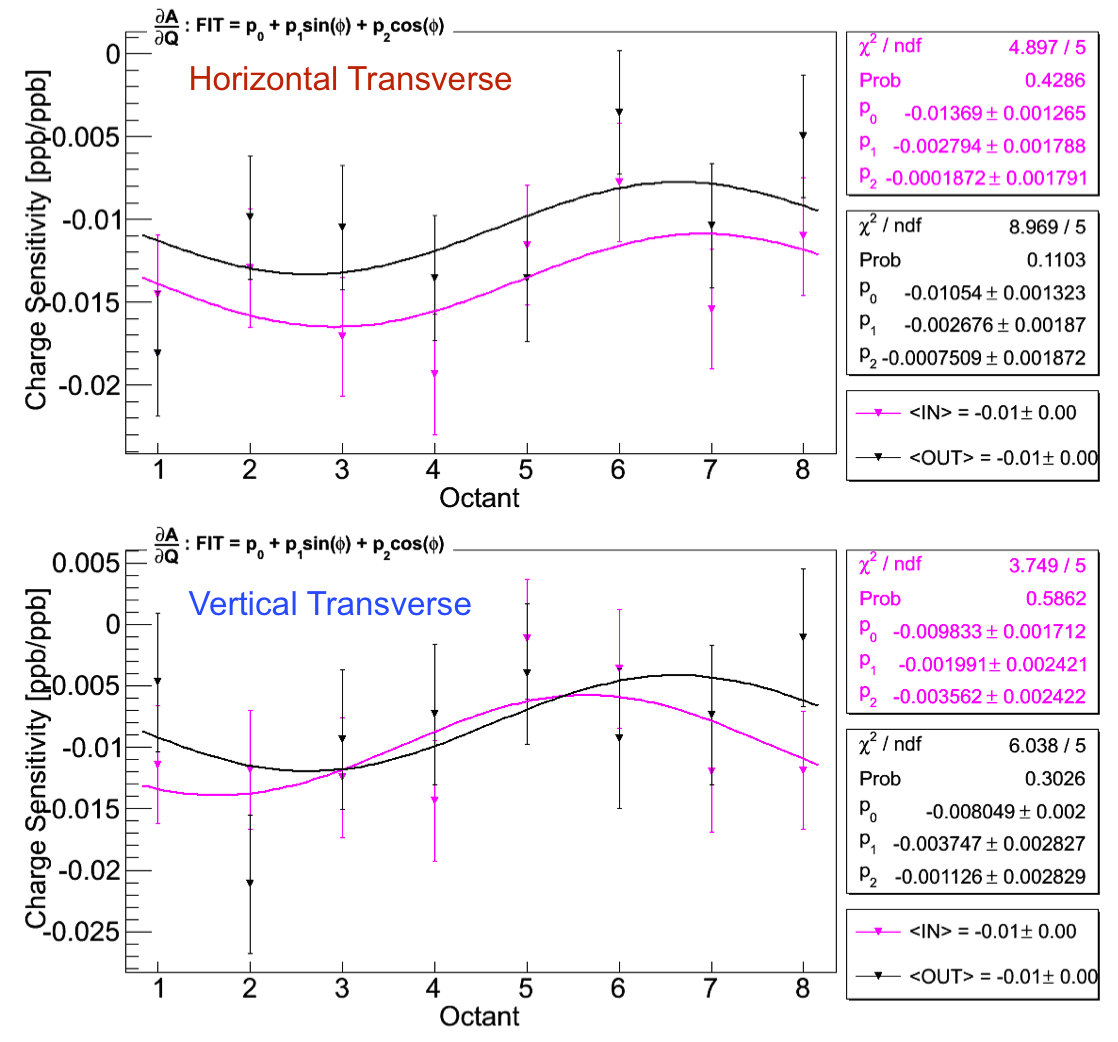
\includegraphics[width=15.0cm]{figures/transverseN2DeltaChargeSensitivity}
	\end{center}
	\caption
%	[Charge sensitivity for horizontal and vertical transverse polarization data set.]
	{Charge sensitivity for horizontal (top) and vertical (bottom) transverse polarization data set. Average charge sensitivities of the measured detector asymmetries extracted from the six parameter (five parameter + charge) regression at beam current 180~$\mu$A. Purple (Black) represents the charge sensitivity of the IHWP IN (OUT) data which are consistent with each other. The sensitivities of the eight \v{C}erenkov detectors vary from -0.5\% to - 2.0\% and are stable within the running period. Average non linearity is -1\% for both the cases.}
	\label{fig:transverseN2DeltaChargeSensitivity}
\end{figure}

\subsection{Nonlinearity}
\label{Nonlinearity}
The \v{C}erenkov detector signals are normalized to the charge and the charge asymmetry is actively suppressed using a charge feedback system. The nonlinearity of the BCM electronics, the main detector electronics, and target density changes can induce nonlinear distortions in the charge asymmetry and hence in the measured asymmetry~\cite{mack_BCMLinearity}. This nonlinearity of the system is seen to be non-zero from the non-zero charge sensitivity constant term in the ``5+1" regressed detector asymmetries, as shown in Figure~\ref{fig:transverseN2DeltaChargeSensitivity}. For both horizontal and vertical polarization data sets, the nonlinearity is found to be -1\%. At present, no proper method of handling the measured asymmetry distortion due to nonlinearity is available. The nonlinearity term is multiplied with the measured asymmetry to calculate the false asymmetry~\cite{mack_nonlinearity}. The systematic uncertainties due to nonlinearity for horizontal and vertical transverse measurements are given by 0.053~ppm and 0.045~ppm, respectively.


\begin{figure}[!h]
	\begin{center}
	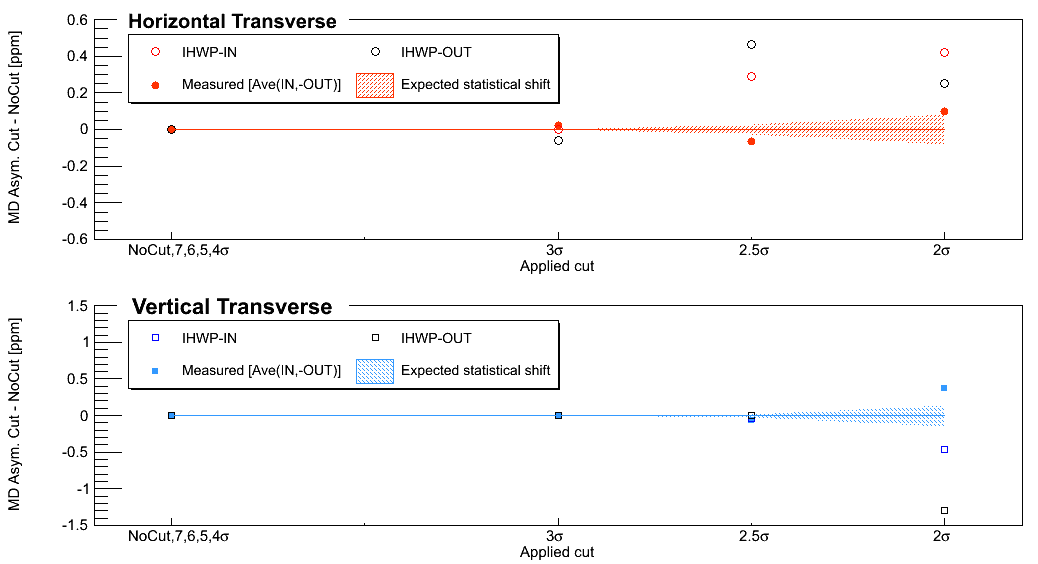
\includegraphics[width=15.0cm]{figures/cutDependence_LH2}
	\end{center}
	\caption
%	[Cut dependence study.]	
	{Cut dependence study. Shift in the central value of the regressed asymmetry for different cut widths for LH$_{2}$. The expected statistical shift is shown by the shaded region using the total number of quartets lost when a cut is applied to all parameters.}
	\label{fig:cutDependence_LH2}
\end{figure}

\subsection{Cut Dependence}
\label{Cut Dependence}
The goal of the cut dependence analysis was to assign a systematic uncertainty that comes from shifts in the mean value of the regressed asymmetry beyond statistical fluctuations after applied cuts. If linear regression is working properly, large false asymmetries in runlets with large HCBAs should be removed from the measured asymmetry after linear regression is applied and there should not be any shift in the mean value of the regressed asymmetry beyond statistical shifts (as shown in Figure~\ref{fig:cutDependence_LH2}).
The point-to-point uncertainty in going from cut $i$ to cut $j$ is estimated to be

\begin{equation} \label{equ:eqCutDependence1}
\Delta_{i \rightarrow j}^{\rm pt-to-pt} = \left( \frac{\sigma_{j}}{\sqrt{N_{j}}} - \frac{\sigma_{i}}{\sqrt{N_{i}}} \right)
\end{equation}

%Cuts on the helicity-correlated beam parameters were used to assign a systematic error that comes from shifts in the mean value of the regressed (5+1) asymmetry after cuts are applied.

Here the $\sigma$ is the root mean square (RMS) of each HCBA.
Inclusive cuts of 7, 6, 5, 4, 3, 2.5 and 2$\sigma$ are applied to all HCBAs and difference between regressed asymmetry with cut and without cuts are shown in Figure~\ref{fig:cutDependence_LH2}.
The observed shift in the measured asymmetry from these cuts are larger than the expected statistical shift and 2.5$\sigma$ cuts on the HCBAs were used to assign a systematic uncertainty. The total percentage of quartets lost for cuts with respect to no cut are used to estimate the expected statistical shift, shown as the shaded region in Figure~\ref{fig:cutDependence_LH2}. Beyond a cut of 2.5$\sigma$, most of the data were removed to extract a meaningful asymmetry. This analysis was performed to assign systematic uncertainty only, no data was removed from main data set. 
Cut dependence for horizontal and vertical transverse data set are found to be $\sim$0.064~ppm and $\sim$0.068~ppm, respectively.

%\begin{center}
%\framebox[\frameboxsize][c]{Cut dependence is $\sim$0.0654~ppm.}
%\end{center}

\subsection{Fit Scheme Dependence}
\label{Fit Scheme Dependence}
A sinusoidal fit to main detector octant asymmetries is used to extract measured transverse asymmetry. So it was important to find the impact of the function on fitted asymmetry.
The measured asymmetry was fitted using four different functions, and the solutions are summarized in Table~\ref{tab:FitSchemeDependence}. 
%The phase of the fit can also affect extracted asymmetry. In this analysis two methods were used, first by fitting the phase as a parameter and  second without fitting the phase. 
%Different fit functions and corresponding measured asymmetries are shown Table~\ref{tab:FitSchemeDependence}. 
The difference in measured asymmetry obtained using standard function $\epsilon_{M}\sin(\phi+\phi_{0})+C$ and rest gives an idea about the fit function dependence of the measured asymmetry. More insightfully, the constant term in the fit function can be thought of as the apparent parity violating asymmetry contamination to the parity conserving transverse asymmetry. The size of $P_{T}B_{n}$ is much larger than $P_{L}A_{\rm PV}$ so the latter has significant effect on the transverse measurement. So this PV asymmetry is buried under the fit scheme dependence and give rise to the systematic uncertainties of 0.040~ppm for horizontal and 0.083~ppm for vertical transverse data sets. 

%\begin{table}[!h]
%\begin{center}
%  	\caption
%	[Fit scheme dependence of the measured asymmetry.]
%  	{Fit scheme dependence of the measured asymmetry. The fit function was varied to observe the effect on measured regressed asymmetry. The difference in asymmetry between case 1 and rest are shown. Biggest offset comes from the possible phase shift.}
%  \begin{tabular}{ c | c  c  c  | c  c  c }
%%    \hline
%    \noalign{\hrule height 1pt}
% 	& \multicolumn{3}{c|}{Horizontal transverse}  & \multicolumn{3}{c}{Vertical transverse} \\ 
%% 	\hline
%	\cline{2-7}
%    & \multirow{3}{*}{Fit Function} 	& \multirow{2}{*}{$A_{M}^{H}$}	&	Difference 	& \multirow{3}{*}{Fit Function} &	\multirow{2}{*}{$A_{M}^{V}$}	&	Difference \\
%    	&		 		&					&	(1-i)			& &				&	(1-i) \\
%    	&		 		&	[ppm]				&	[ppm]			& &	[ppm]				&	[ppm] \\
%%    	 \hline
%    \noalign{\hrule height 1pt}
%	1 & $A_{M}^{H}\sin(\phi+\phi_{0}^{H})+C^{H}$	& 5.343 &0.000 & $A_{M}^{V}\cos(\phi+\phi_{0}^{V})+C^{V}$	& 4.525 &	 0.000 \\
%	2 & $A_{M}^{H}\sin(\phi+\phi_{0}^{H})$ & 5.344 & 0.001 & $A_{M}^{V}\cos(\phi+\phi_{0}^{V})$ & 4.510 &	 0.015 \\
%	3 & $A_{M}^{H}\sin(\phi)+C^{H}$ & 5.303 & 0.040 & $A_{M}^{V}\cos(\phi)+C^{V}$ & 4.458 & 0.067 \\
%	4 & $A_{M}^{H}\sin(\phi)$ & 5.304 & 0.039 & $A_{M}^{V}\cos(\phi)$ & 4.442 &	 0.083 \\	
%%    \hline
%    \noalign{\hrule height 1pt}
%  	\end{tabular}
%  \label{tab:FitSchemeDependence}
%\end{center}
%\end{table}


\begin{table}[!h]
\begin{center}
  	\caption
%	[Fit scheme dependence of the measured asymmetry.]
  	{Fit scheme dependence of the measured asymmetry. The fit function was varied to observe the effect on measured regressed asymmetry. The difference in asymmetry between case 1 and rest are shown. Biggest offset comes from the possible phase shift.}
  \begin{tabular}{ c | c  c  c }
    \noalign{\hrule height 1pt}
% 	& \multicolumn{3}{c|}{Horizontal transverse}  & \multicolumn{3}{c}{Vertical transverse} \\ 
%	\cline{2-7}
    & \multirow{3}{*}{Fit Function} 	& \multirow{2}{*}{Asymmetry}	&	Difference \\
    	&		 		&						&	(1-i)		\\
    	&		 		&	[ppm]				&	[ppm]	\\
    \noalign{\hrule height 1pt}
    \multicolumn{4}{c}{Horizontal Transverse} \\
    \hline
	1 & $\epsilon_{M}^{H}\sin(\phi+\phi_{0}^{H})+C^{H}$	& 5.343 $\pm$ 0.532	& 0.000 \\
	2 & $\epsilon_{M}^{H}\sin(\phi+\phi_{0}^{H})$ 		& 5.344 $\pm$ 0.532	& 0.001 \\
	3 & $\epsilon_{M}^{H}\sin(\phi)+C^{H}$ 				& 5.303 $\pm$ 0.533 	& 0.040 \\
	4 & $\epsilon_{M}^{H}\sin(\phi)$ 					& 5.304 $\pm$ 0.533 	& 0.039 \\	
    \noalign{\hrule height 1pt}
    \multicolumn{4}{c}{Vertical Transverse} \\
    \hline
	1 & $\epsilon_{M}^{V}\cos(\phi+\phi_{0}^{V})+C^{V}$	& 4.525 $\pm$ 0.806 	& 0.000 \\
	2 & $\epsilon_{M}^{V}\cos(\phi+\phi_{0}^{V})$ 		& 4.510 $\pm$ 0.806 	& 0.015 \\
	3 & $\epsilon_{M}^{V}\cos(\phi)+C^{V}$ 				& 4.458 $\pm$ 0.807	& 0.067 \\
	4 & $\epsilon_{M}^{V}\cos(\phi)$ 					& 4.442 $\pm$ 0.807	& 0.083 \\	
    \noalign{\hrule height 1pt}
  	\end{tabular}
  \label{tab:FitSchemeDependence}
\end{center}
\end{table}


\begin{figure}[!h]
	\begin{center}
	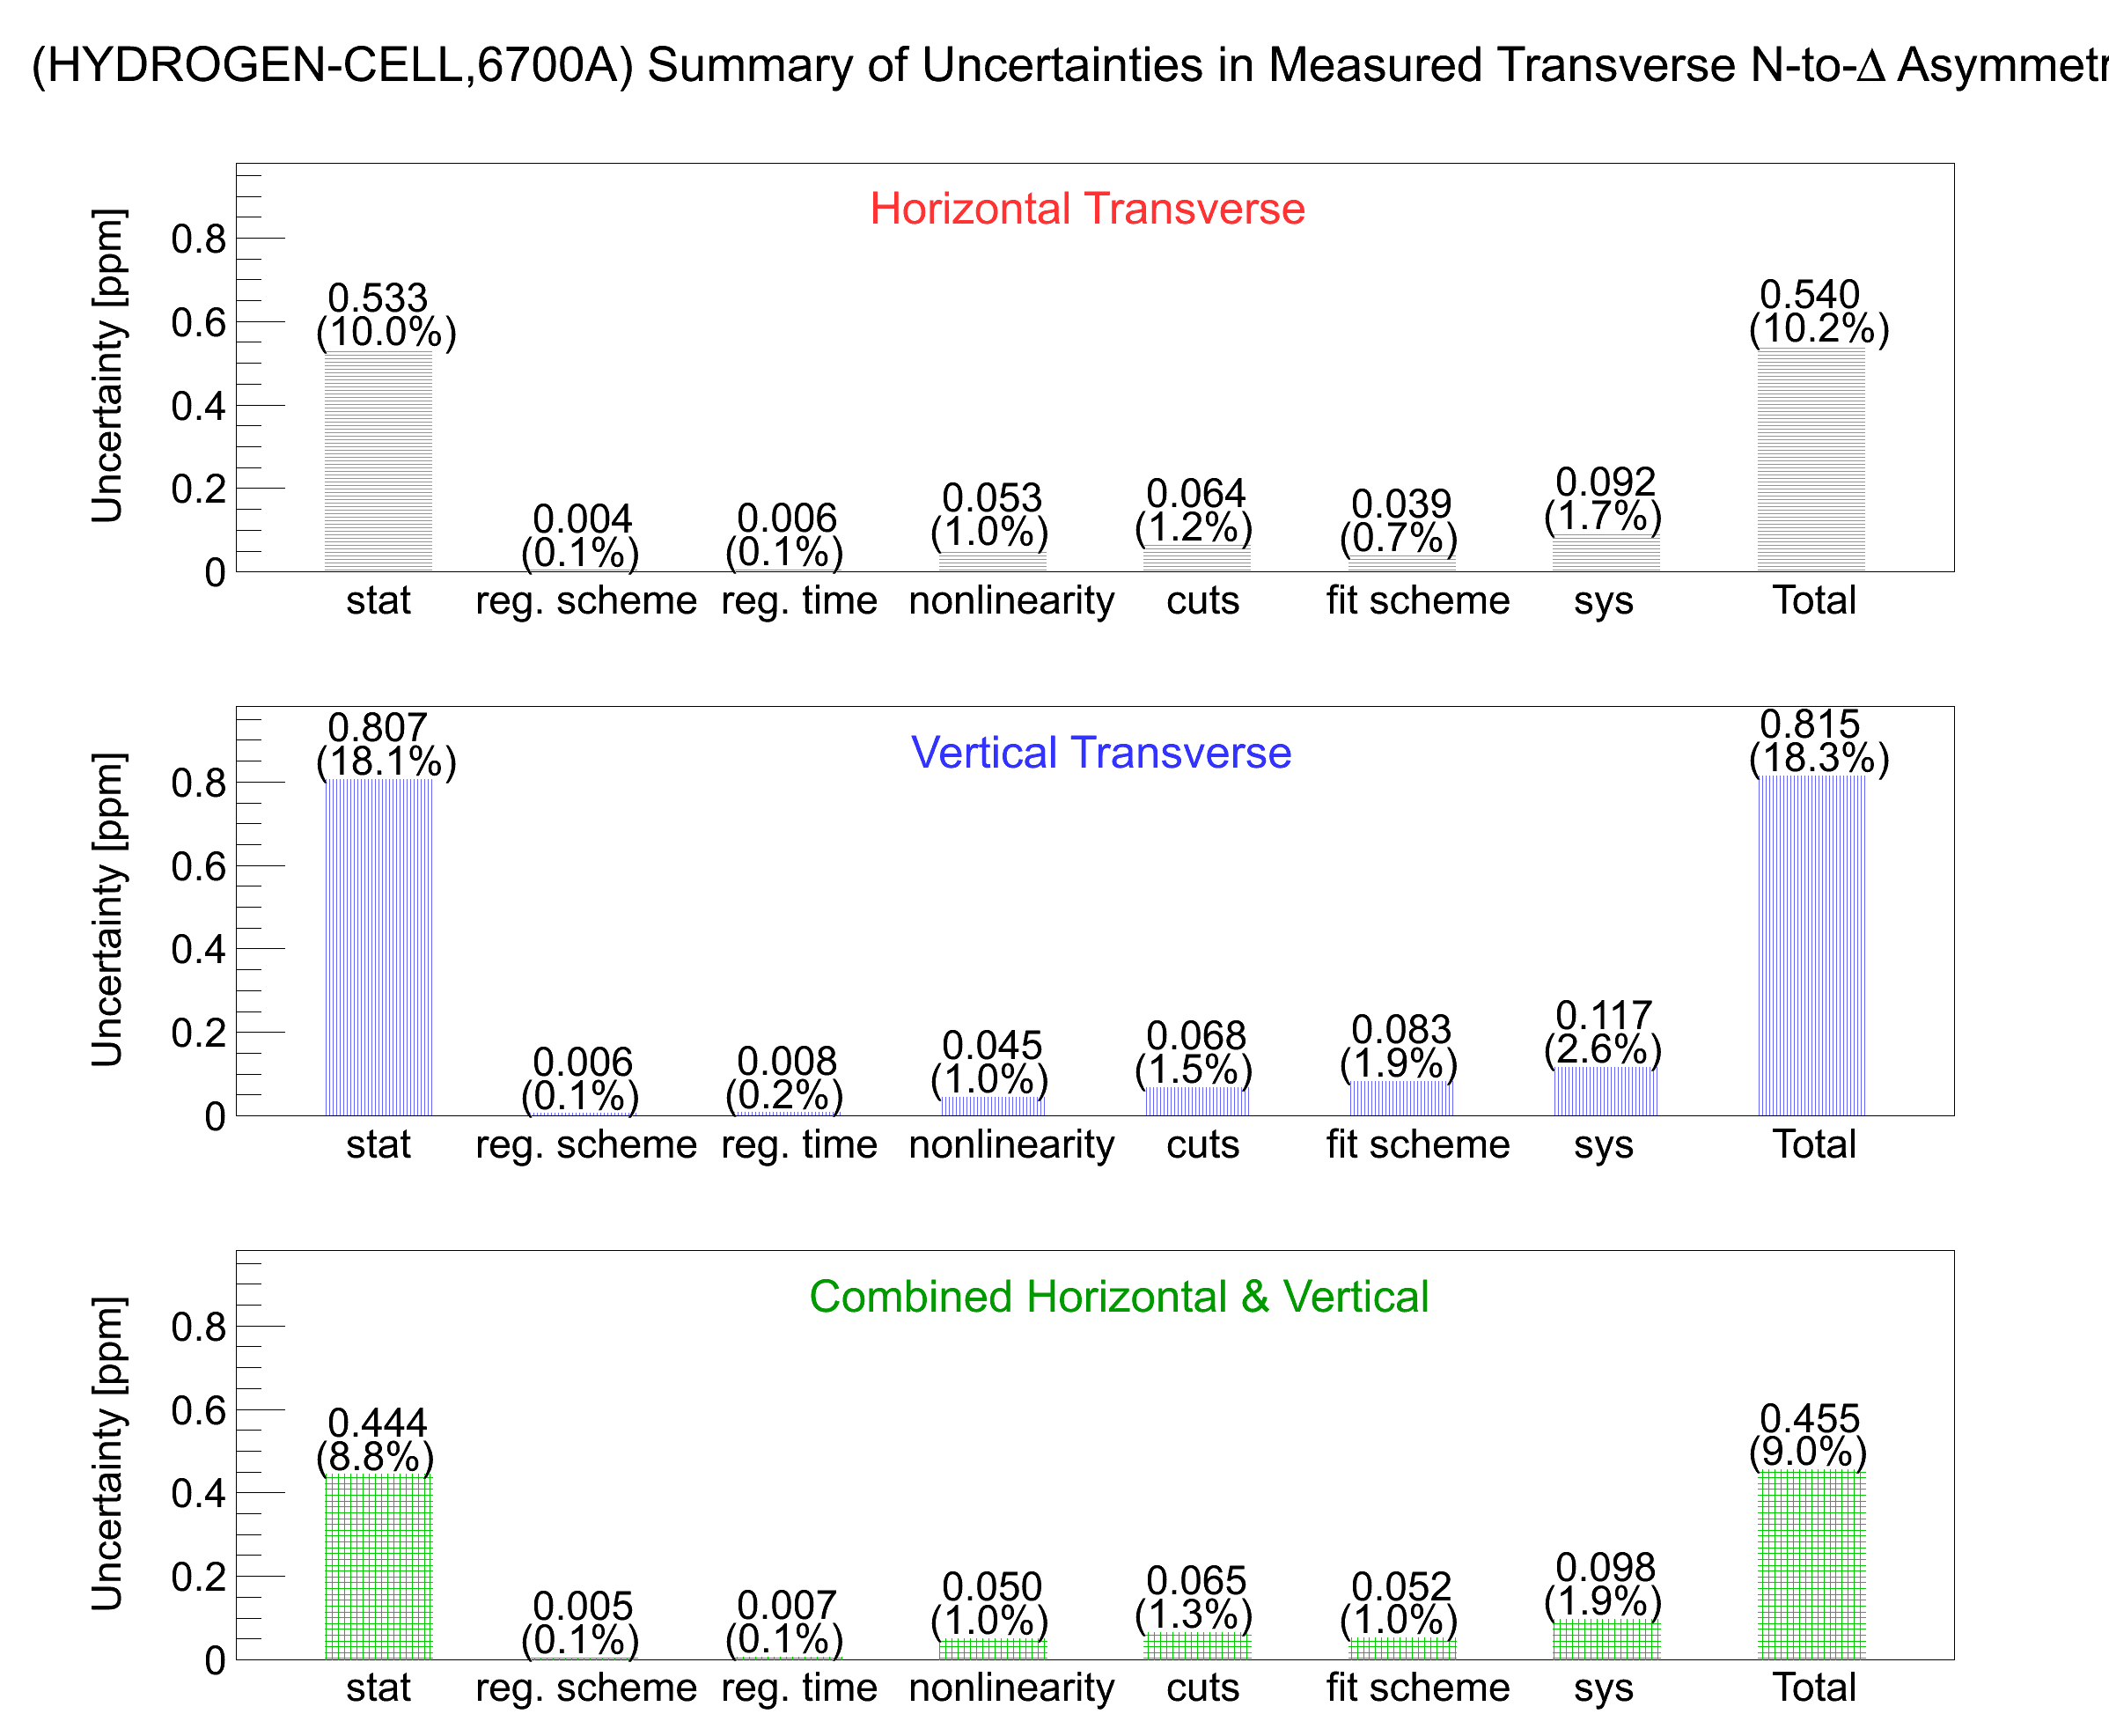
\includegraphics[width=15.0cm]{figures/errorChart}
	\end{center}
	\caption
%	[Summary of uncertainties on measured asymmetry for horizontal and vertical data set.]
	{Summary of uncertainties on measured asymmetry for horizontal and vertical data set. The relative total uncertainty is dominated by statistical uncertainty compared to systematic uncertainties.}
	\label{fig:errorChart}
\end{figure}

\subsection{Summary of Systematic Uncertainties}
\label{Summary of Systematic Uncertainties}
Summary of systematic uncertainties of the measured inelastic beam normal single spin asymmetry is given in Table~\ref{tab:systematic_error}. The systematic studies contain uncertainties related to the extraction of the measured asymmetry such as regression, nonlinearity, cut dependence, and detector acceptance correction. The systematic studies for horizontal and vertical transverse polarization data set were performed separately; these are summarized in Figure~\ref{fig:errorChart}. The statistical uncertainty weighted average of the systematic uncertainties from horizontal and vertical transverse data sets is used for the total systematic uncertainty. The total uncertainty is the quadrature sum of the statistical and systematic uncertainties. The total uncertainty is dominated by 9\% statistical uncertainty compared to 1\% systematic uncertainty.

%\begin{equation} \label{equ:measuredAsymmetry}
%A_{M}^{in} = 5.127~\pm~0.444~\text{(stat)}~\pm~0.100~\text{(sys) ppm}.
%\end{equation}

\begin{table}[!h]
\begin{center}
  	\caption
%  	[Summary of uncertainties on measured asymmetry for combined horizontal and vertical data sets.]
  	{Summary of uncertainties on measured asymmetry for combined horizontal and vertical data sets. The relative uncertainties are also shown in the table.}
  \begin{tabular}{ c | c | c }
%    \hline
    \noalign{\hrule height 1pt}
    \multirow{2}{*}{Uncertainty from}&	Contribution to $\epsilon_{M}$	&	Relative Contribution 	\\
									&	[ppm]	&	[\%] \\ 
%	\hline
    \noalign{\hrule height 1pt}
 	Statistics   					&	0.444	&	8.8	\\ 
% 	\hline
    \noalign{\hrule height 1pt}
	Regression scheme   				&	0.005	& 	0.1	\\
	Regression time binning			&	0.007	&	0.1	\\
	Non-linearity					&	0.050	& 	1.0	\\
	Cuts 							&	0.065	& 	1.3	\\
	Fit scheme 						&	0.052	& 	1.0	\\ 
%	Detector acceptance correction	&	0.016	& 	0.3	\\ 
	\hline
%    \noalign{\hrule height 1pt}
	Systematic only					&	0.098	& 	1.9	\\ 
%	\hline
    \noalign{\hrule height 1pt}
	Total 							& 	0.455 	& 	9.0	\\    	
%    \hline
    \noalign{\hrule height 1pt}
  	\end{tabular}
  \label{tab:systematic_error}
\end{center}
\end{table}

%\begin{table}[!h]
%\begin{center}
%  \begin{tabular}{ c  c  c }
%    \hline
%    Error from	&	Contribution to $A_{M}$		&	Section	\\
%														&	[ppm]	&	\\\hline
%	Regression scheme dependence  &	0.005	& 	\ref{Regression Scheme Dependence}	\\
%	Regression time dependence		&	0.007	&	\ref{Regression Time Dependence} \\
%	Cut dependence							&	0.065	& \ref{Cut Dependence} \\
%	Non-linearity								&	0.051	& \ref{Cut Dependence} \\
%	Fit scheme dependence				&	0.052	& \ref{Fit Scheme Dependence} \\\hline
%
%	Total 											& 	0.127 	& \\    	
%    \hline
%  	\end{tabular}
%  	\caption[Systematic error table.]{Systematic error table.}
%  \label{tab:systematic_error}
%\end{center}
%\end{table}


%\newpage
%%%%%%%%%%%%%%%%%%%%%%%%%%%%%%%%%%%%%%%%%%%%%%%%%%%%%%%%%%%%%
\section{Extraction of Physics Asymmetry}
\label{Extraction of Physics Asymmetry}
%
%\begin{landscape}
%
%%\begin{flushleft}
%\begin{table}[h]
%\begin{center}
%  \begin{tabular}{ c | c  c  c | c  c | c  c | c }
%    \hline
%    Quantity 		&	&	Asymmetry	&	& 	& Dilution & Correction & $c_{i}=A_{bi}f_{bi}$ & Reference		\\
%	\hline
%	Aluminum asymmetry & $A_{b1}$ & 8.431 $\pm$ 0.985 & ppm & $f_{b1}$ & 0.033 $\pm$ 0.002 & $c_{b1}$ & 0.033 $\pm$ 0.002 &	\href{https://qweak.jlab.org/elog/Analysis+&+Simulation/451}{ELOG 451 (Analysis)}\cite{website:elog_adesh} \\
%
%	QTOR transport channel & $A_{b2}$ & 0.000 $\pm$ 0.000 & ppm	& $f_{b2}$ & 0.033 $\pm$ 0.002 & $c_{b1}$ & 0.033 $\pm$ 0.002 & \href{https://qweak.jlab.org/doc-private/ShowDocument?docid=1655}{DocDB 1655} \cite{buddhini_transverse_technote}	\\
%
%	Beamline background & $A_{b3}$ & 0.000 $\pm$ 0.000 & ppm	& $f_{b3}$ & 0.033 $\pm$ 0.002 & $c_{b1}$ & 0.033 $\pm$ 0.002 & 	\href{https://qweak.jlab.org/doc-private/ShowDocument?docid=1655}{DocDB 1655} \cite{buddhini_transverse_technote}	\\
%	
%	Elastic asymmetry & $A_{b4}$ & -5.305 $\pm$ 0.166 & ppm	& $f_{b4}$ & 0.033 $\pm$ 0.002 & $c_{b1}$ & 0.033 $\pm$ 0.002 &	\href{https://qweak.jlab.org/doc-private/ShowDocument?docid=1655}{DocDB 1655} \cite{buddhini_transverse_technote}	\\
%
%    \hline
%  	\end{tabular}
%  	\caption[Background correction table.]{Background correction table.}
%  \label{tab:PhysicsAsymInput}
%\end{center}
%\end{table}
%%\end{flushleft}
%
%
%
%\begin{table}[h]
%\begin{center}
%  \begin{tabular}{ c  c  c  c  c  c  c }
%    \hline
%    Quantity 		&	&	Value	&	&	& &  Reference		\\
%	\hline
%	Inelastic measured asymmetry & $A^{in}_{M}$ &	4.789 $\pm$ 0.844 & ppm & & & This analysis\\
%
%	Polarization & P & 	0.879 $\pm$ 0.018 & &	& & \href{https://qweak.jlab.org/doc-private/ShowDocument?docid=1655}{DocDB 1655} \cite{buddhini_transverse_technote}	\\
%
%	Aluminum asymmetry & $A_{b1}$ & 8.431 $\pm$ 0.985 & ppm & $f_{b1}$ & 0.033 $\pm$ 0.002 &	This analysis\\
%	
%%	Aluminum dilution factor & $f_{b1}$ & 0.033 $\pm$ 0.002 & &	\href{https://qweak.jlab.org/elog/Analysis+&+Simulation/451}{ELOG 451 (Analysis)}\cite{website:elog_adesh}	\\
%
%%	Aluminum asymmetry radiative correction & $R^{A}_{b1}$ & 1.000 $\pm$ 0.000 &		&	Place holder	\\
%
%	QTOR transport channel & $A_{b2}$ & 0.000 $\pm$ 0.000 & ppm	& $f_{b1}$ & 0.033 $\pm$ 0.002 & \href{https://qweak.jlab.org/doc-private/ShowDocument?docid=1655}{DocDB 1655} \cite{buddhini_transverse_technote}	\\
%	
%%	QTOR transport channel neutral dilution & $f_{b2}$ & 0.724 $\pm$ 0.004 & &	\href{https://qweak.jlab.org/elog/Analysis+&+Simulation/451}{ELOG 451 (Analysis)}\cite{website:elog_adesh}	\\
%
%	Beamline background & $A_{b3}$ & 0.000 $\pm$ 0.000 & ppm	& $f_{b1}$ & 0.033 $\pm$ 0.002 & 	\href{https://qweak.jlab.org/doc-private/ShowDocument?docid=1655}{DocDB 1655} \cite{buddhini_transverse_technote}	\\
%	
%%	Beamline background dilution & $f_{b3}$ & 0.724 $\pm$ 0.004 & &	\href{https://qweak.jlab.org/elog/Analysis+&+Simulation/451}{ELOG 451 (Analysis)}\cite{website:elog_adesh}	\\
%	
%	Elastic asymmetry & $A_{b4}$ & -5.305 $\pm$ 0.166 & ppm	& $f_{b1}$ & 0.033 $\pm$ 0.002 &	\href{https://qweak.jlab.org/doc-private/ShowDocument?docid=1655}{DocDB 1655} \cite{buddhini_transverse_technote}	\\
%	
%%	Elastic dilution factor & $f_{b4}$ & 0.724 $\pm$ 0.004 & &	\href{https://qweak.jlab.org/elog/Analysis+&+Simulation/451}{ELOG 451 (Analysis)}\cite{website:elog_adesh}	\\
%
%%	Elastic asymmetry radiative correction & $R^{A}_{b4}$ & 1.000 $\pm$ 0.000 &		&	Place holder	\\
%%
%%	EM radiative correction & $M_{RC}$ & 1.000 $\pm$ 0.000 &		&	Place holder	\\
%%
%%	Detector bias correction & $M_{Det}$ & 1.000 $\pm$ 0.000 &		&	Place holder	\\
%
%    \hline
%  	\end{tabular}
%  	\caption[Input table.]{Input table.}
%  \label{tab:PhysicsAsymInput}
%\end{center}
%\end{table}
%
%\end{landscape}
%
%%%%%%%%%%%%%%%%%%%%%%%%%%%%%%%%%%%%%%%%%%%%%%
The beam normal single spin asymmetry from inelastic e+p scattering is obtained from measured asymmetry using Equation~\ref{equ:PhysicsAsymmetryShort} by accounting for EM radiative corrections, kinematics normalization, polarization, and backgrounds.

%\begin{equation} \label{equ:PhysicsAsymmetry}
%A_{N} = M_{RC}M_{Det}M_{Q^{2}}M_{\phi} \left[ \frac{\frac{A^{in}_{M}}{P} - A_{b1}f_{b1} - A_{b2}f_{b2} - A_{b3}f_{b3} - A_{b4}f_{b4} }{1 - f_{b1} - f_{b2} - f_{b3} - f_{b4}} \right] 
%\end{equation}

\begin{equation} \label{equ:PhysicsAsymmetryShort}
B_{n} = M_{total} \left[ \frac{\left(\frac{\epsilon_{reg}}{P}\right) - \sum^{4}_{i=1} B_{bi}f_{bi} }{ 1 -\sum^{4}_{i=1} f_{bi} } \right]
\end{equation}

Here $M_{total}$ is a correction factor for the experimental bias and radiative effects, $P$ is the beam polarization, and $B_{bi}$ is $i^{th}$ background asymmetry with fraction of backgrounds in the total detector acceptance (dilution) $f_{bi}$. The corrections to the physics asymmetry and the associated uncertainties are discussed in the following sections.


\subsection{Beam Polarization}
\label{Beam Polarization}
The Hall-C M{\o}ller polarimeter and the Compton polarimeter were used to measure the beam polarization for the experiment. 
The photocathode Quantum Efficiency was stable and hence the beam polarization was stable for the period~\cite{magee_communication}. 
%The assumptions was that, the beam polarization in the beam within few hours remain similar. 
The M{\o}ller polarimeter is only sensitive to longitudinally polarized beam, so measurements performed with the longitudinally polarized beam right after the transverse data taking was used to determine the beam polarization. 
%The M{\o}ller measurements performed with the longitudinally polarized beam right after the the transverse data taking was used to determine the beam polarization. 
The M{\o}ller runs used for this analysis are 1593 - 1599, carried out on 20th February 2012. Each run is $\sim$10 min long. Slug averaged polarizations from this M{\o}ller measurement are shown in Table~\ref{tab:polarization}. The measured beam polarization is $P$ = 87.50 $\pm$ 0.28 (stat) $\pm$ 0.74 (sys)\%~\cite{elog:nur_ancillary91}. Details of systematic studies for the M{\o}ller polarization measurement can be found in the Q-weak internal technical document~\cite{magee_moller}.
%~\cite{magee_communication}

\begin{table}[h]
\begin{center}
  	\caption
%	[Beam polarization using M{\o}ller polarimeter for Run 2 transverse data set.]  	
  	{Beam polarization using M{\o}ller polarimeter for Run 2 transverse data set~\cite{magee_moller}.}
  \begin{tabular}{ c | c | c }
%    \hline
    \noalign{\hrule height 1pt}
    \multirow{2}{*}{IHWP} &	Polarization		&	Statistical Uncertainty	\\
    			&	[\%]					&	[\%]		\\ 
%    	\hline
    \noalign{\hrule height 1pt}
	Out 		& 87.029 				& 0.398	\\
	In 		& - 87.939 			& 0.387	\\ 
%	\hline
    \noalign{\hrule height 1pt}
	Total 	& 87.497 				& 0.277	\\ 
%	\hline
    \noalign{\hrule height 1pt}
  	\end{tabular}
  \label{tab:polarization}
\end{center}
\end{table}


%M{\o}ller polarimeter is only sensitive to longitudinal polarization.
%To determine the beam polarization in the transversely polarized beam, the experiment relied on M{\o}ller measurements done with the longitudinally polarized beam close to the transverse data taking period. Since the quantum efficiency of a laser spot on the cathode is good for up to two weeks (see Subsection 3.2.1), the polarization in the beam within one to two days of the transverse measurements are similar to the beam polarization in the transverse running period.
%By design, the Møller polarimeter is only sensitive to longitudinal polarization.
%To determine the beam polarization in the transversely polarized beam, the experiment
%relied on Møller measurements done with the longitudinally polarized beam
%close to the transverse data taking period. Since the quantum efficiency of a laser
%spot on the cathode is good for up to two weeks (see Subsection 3.2.1), the polarization
%in the beam within one to two days of the transverse measurements are similar to
%the beam polarization in the transverse running period. With this assumption, Transverse
%Run I uses the beam polarization estimated [148] for the Qweak 21 % result from
%the commissioning period (see left panel in Figure 6.15).
%Table 6.8 shows the polarization results from run2 used for the transverse analysis.

%\begin{figure}[!h]
%	\begin{center}
%	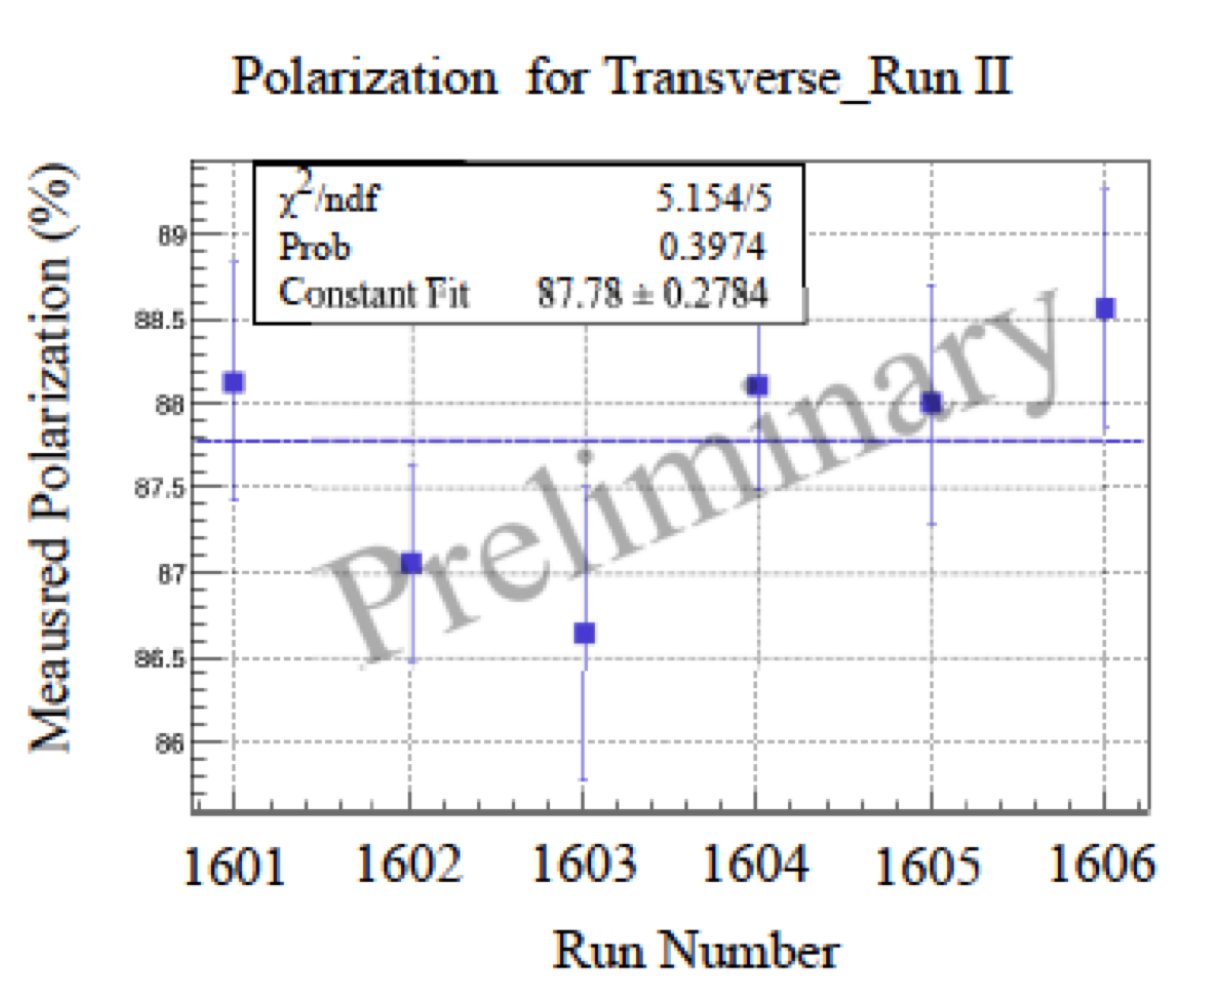
\includegraphics[width=10.0cm]{figures/beamPolarization}
%	\end{center}
%	\caption[Polarization results used for transverse dataset based on the M{\o}ller measurements performed on
%February 20th, 2012 immediately after transverse measurements. The uncertainties shown are statistical only. The data points are corrected for IHWP reversal.]{Polarization results used for transverse dataset based on the M{\o}ller measurements performed on
%February 20th, 2012 immediately after transverse measurements. The uncertainties shown are statistical only. The data points are corrected for IHWP reversal.}
%	\label{fig:beamPolarization}
%\end{figure}



\subsection{Background Corrections}
\label{Background Corrections}

The largest background source in beam normal single spin asymmetry arises from the elastic radiative tail. Small background contributions also come from electrons scattering from aluminum target windows, beamline scattering, and other soft neutral scattering. The analysis of the background asymmetries and their contributions to the BNSSA is described in the following sections.


\begin{figure}[!h]
	\begin{center}
	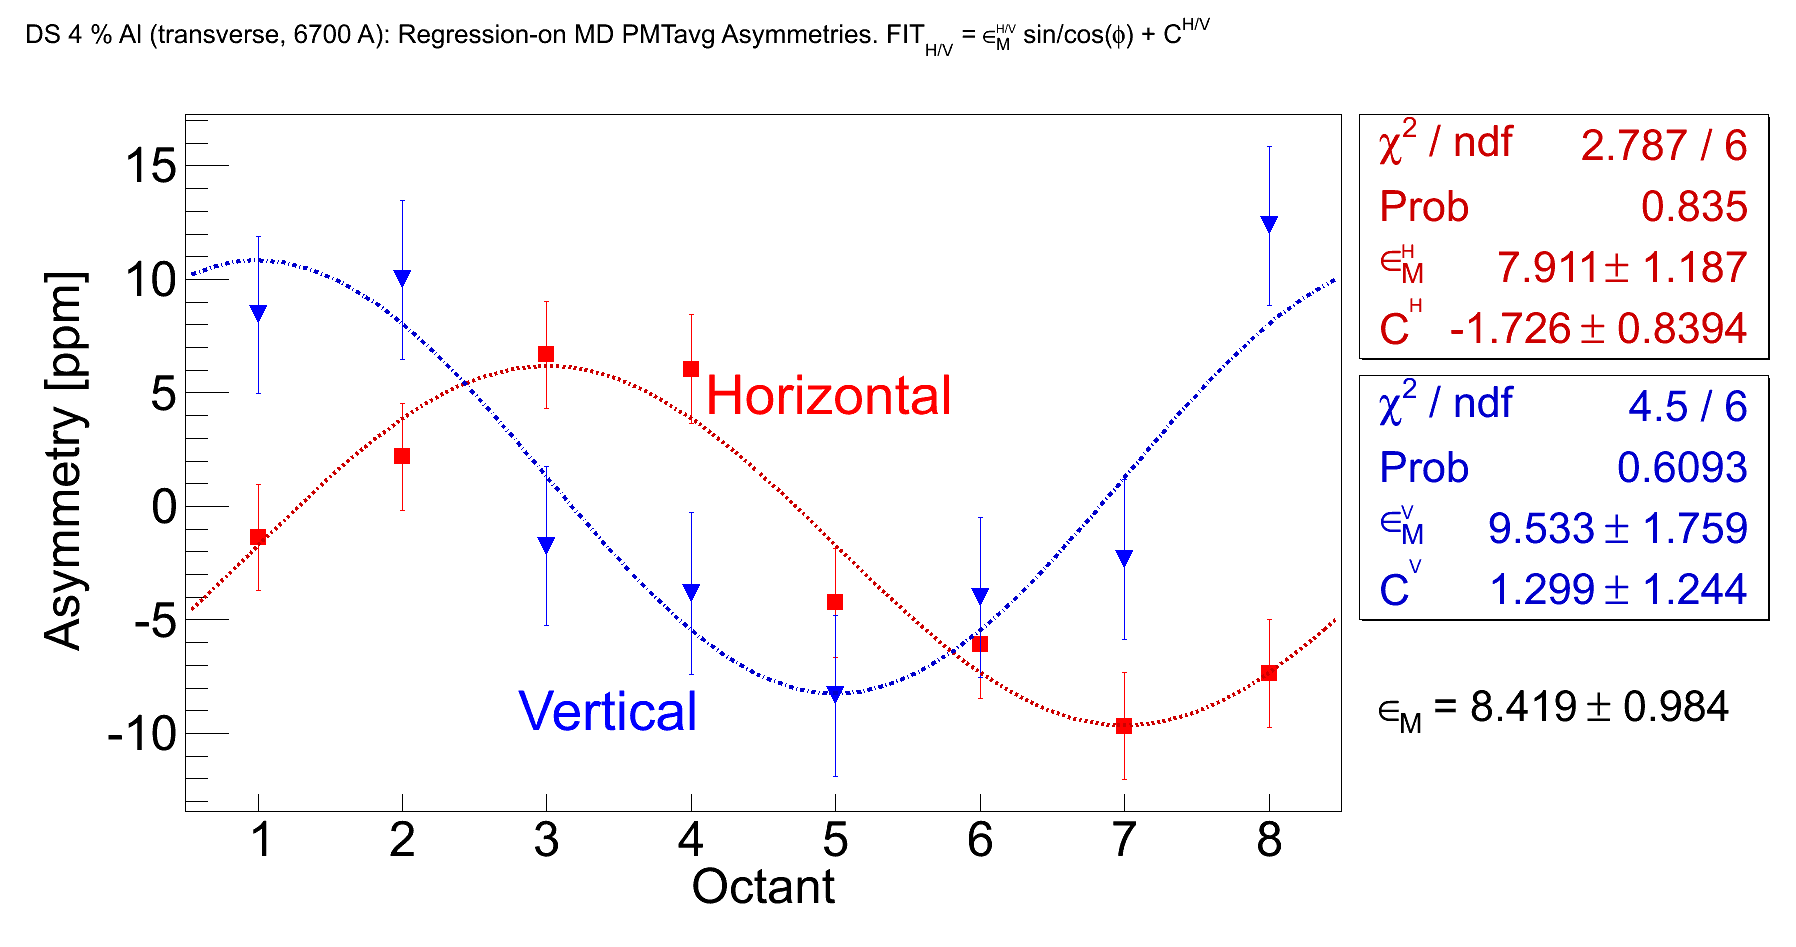
\includegraphics[width=15.0cm]{figures/asymmetry_Al}
	\end{center}
	\caption
%	[Azimuthal dependence of asymmetry from the 4\% downstream aluminum target.]
	{Azimuthal dependence of asymmetry from the 4\% downstream aluminum target. The uncertainties are statistical only. The octant dependence in either polarization orientation are similar to what was observed for the LH$_{2}$-cell. The asymmetry is larger than the LH$_{2}$-cell asymmetry. The fit functions used for horizontal and vertical transverse data points are $\epsilon_{M}^{H}\sin(\phi+\phi_{0}^{H}) + C^{H}$ and $\epsilon_{M}^{V}\cos(\phi+\phi_{0}^{V}) + C^{V}$, respectively.}
	\label{fig:asymmetry_Al}
\end{figure}

\subsubsection{Target Aluminum Windows}
\label{Target Aluminum Windows}
One of the important background contributions to the measured asymmetry comes from electrons scattering from the aluminum alloy target windows. 
Data were taken on the 4\% downstream aluminum alloy target to determine the asymmetry and dilution.
%To determine the size of this asymmetry, we took data on the 4\% Downstream aluminum target. 
The measured regressed asymmetry for horizontal and vertical transverse are $\epsilon^{H-DSAl}_{M}$ = 7.911~$\pm$~1.187~(stat) $\pm$ 0.482~(sys)~ppm and $\epsilon^{V-DSAl}_{M}$ = 9.533~$\pm$1.759~(stat) $\pm$~0.870~(sys)~ppm~\cite{elog:nur_ancillary43}, as shown in Figure~\ref{fig:asymmetry_Al}. Combined (error weighted) regressed aluminum alloy asymmetry is $\epsilon^{DSAl}_{M}$ = 8.419~$\pm$~0.984~(stat) $\pm$ 0.603~(sys)~ppm. 
The systematic studies for 4\% downstream aluminum alloy target contain uncertainties related to the extraction of the measured asymmetry such as regression, nonlinearity, cut dependence, and detector acceptance correction, as described in section~\ref{Systematic Uncertainties} (see APPENDIX~\ref{Beam Normal Single Spin Asymmetry in Inelastic e-p Scattering} for more details on Al analysis).
%This asymmetry is then scaled by a 0.9938 for azimuthal acceptance averaging (already discussed in section~\ref{Azimuthal Acceptance Correction}), which yields the asymmetry as 8.484 $\pm$ 0.985~ppm. 
The acceptance difference between the upstream and downstream target windows need to correct before the background correction. This acceptance difference causes a 20\% relative difference between the mean $Q^{2}$ of the electrons coming from the upstream window compared to the downstream window, as shown in GEANT4 simulations~\cite{kmyers_qweak} ($Q^{2}_{USAl}$=0.8$\times Q^{2}_{DSAl}$). The beam normal single spin asymmetry from nuclei at forward angle scattering asymmetry is proportional to $\sqrt{Q^{2}}$ as described in theoretical models~\cite{PhysRevC.72.034602, PhysRevC.77.044606}. So, asymmetry for upstream aluminum target can be calculated as $\epsilon^{USAl}_{M}$ = $\sqrt{0.8} \epsilon^{DSAl}_{M}$ = 7.530~ppm. Downstream and upstream aluminum target windows are expected to contribute equally~\cite{kmyers_qweak} to the aluminum dilution in the main detector asymmetries resulting in an effective aluminum asymmetry of $\epsilon^{Al}_{M}$ = $(\epsilon^{DSAl}_{M}+\epsilon^{DSAl}_{M})/2$ = 7.974~ppm. 
%An additional systematic uncertainty of 0.08$\times \epsilon^{Al}_{M}$ is assigned for the system non-linearity (more details in APPENDIX~\ref{Beam Normal Single Spin Asymmetry in Inelastic e-p Scattering}). 
The polarization corrected asymmetry for background windows correction is $B_{Al}$ = $\epsilon^{Al}_{M}$/$P$ = 9.061~$\pm$~1.405~ppm.
%\begin{equation} \label{equ:AluminumAsymmetry}
%A^{in}_{PHYS} = \frac{\frac{A^{in}_{M}}{P} - A^{Al}f^{Al}}{1 - f^{Al}}
%\end{equation}

\begin{table}[h]
\begin{center}
  	\caption
%	[Measured asymmetry on aluminum target.]
  	{Measured asymmetry on aluminum target.}
  \begin{tabular}{ c | c }
%    \hline
    \noalign{\hrule height 1pt}
    \multirow{2}{*}{Target} &	Asymmetry \\
    			&	[ppm]				\\ 
    \noalign{\hrule height 1pt}
	DSAl 	& 8.419 \\
	USAl		& 7.530 	\\ 
    \noalign{\hrule height 1pt}
	$<$DS+US$>$ 	& 7.974 \\ 
    \noalign{\hrule height 1pt}
  	\end{tabular}
  \label{tab:aluminumAsymmetry}
\end{center}
\end{table}


The measured aluminum windows dilution 
%, the fraction of the total rate seen by the main detectors that is from the target's aluminum windows, 
is $f_{Al}$ = 0.033~$\pm$~0.002~\cite{presentation:josh_1891}. 
Dedicated measurements were performed with different pressures of hydrogen gas in the target cell. Using the known pressure of hydrogen gas at different points, the pressure was extrapolated to zero. % Data was also taken with an evacuated target cell. 

The correction to the physics asymmetry from aluminum alloy windows is $c_{Al}$ = $M_{total}B_{Al}f_{Al}/(1-f_{total})$ = 1.416~$\pm$~0.246~ppm.

%\begin{figure}[!h]
%	\begin{center}
%	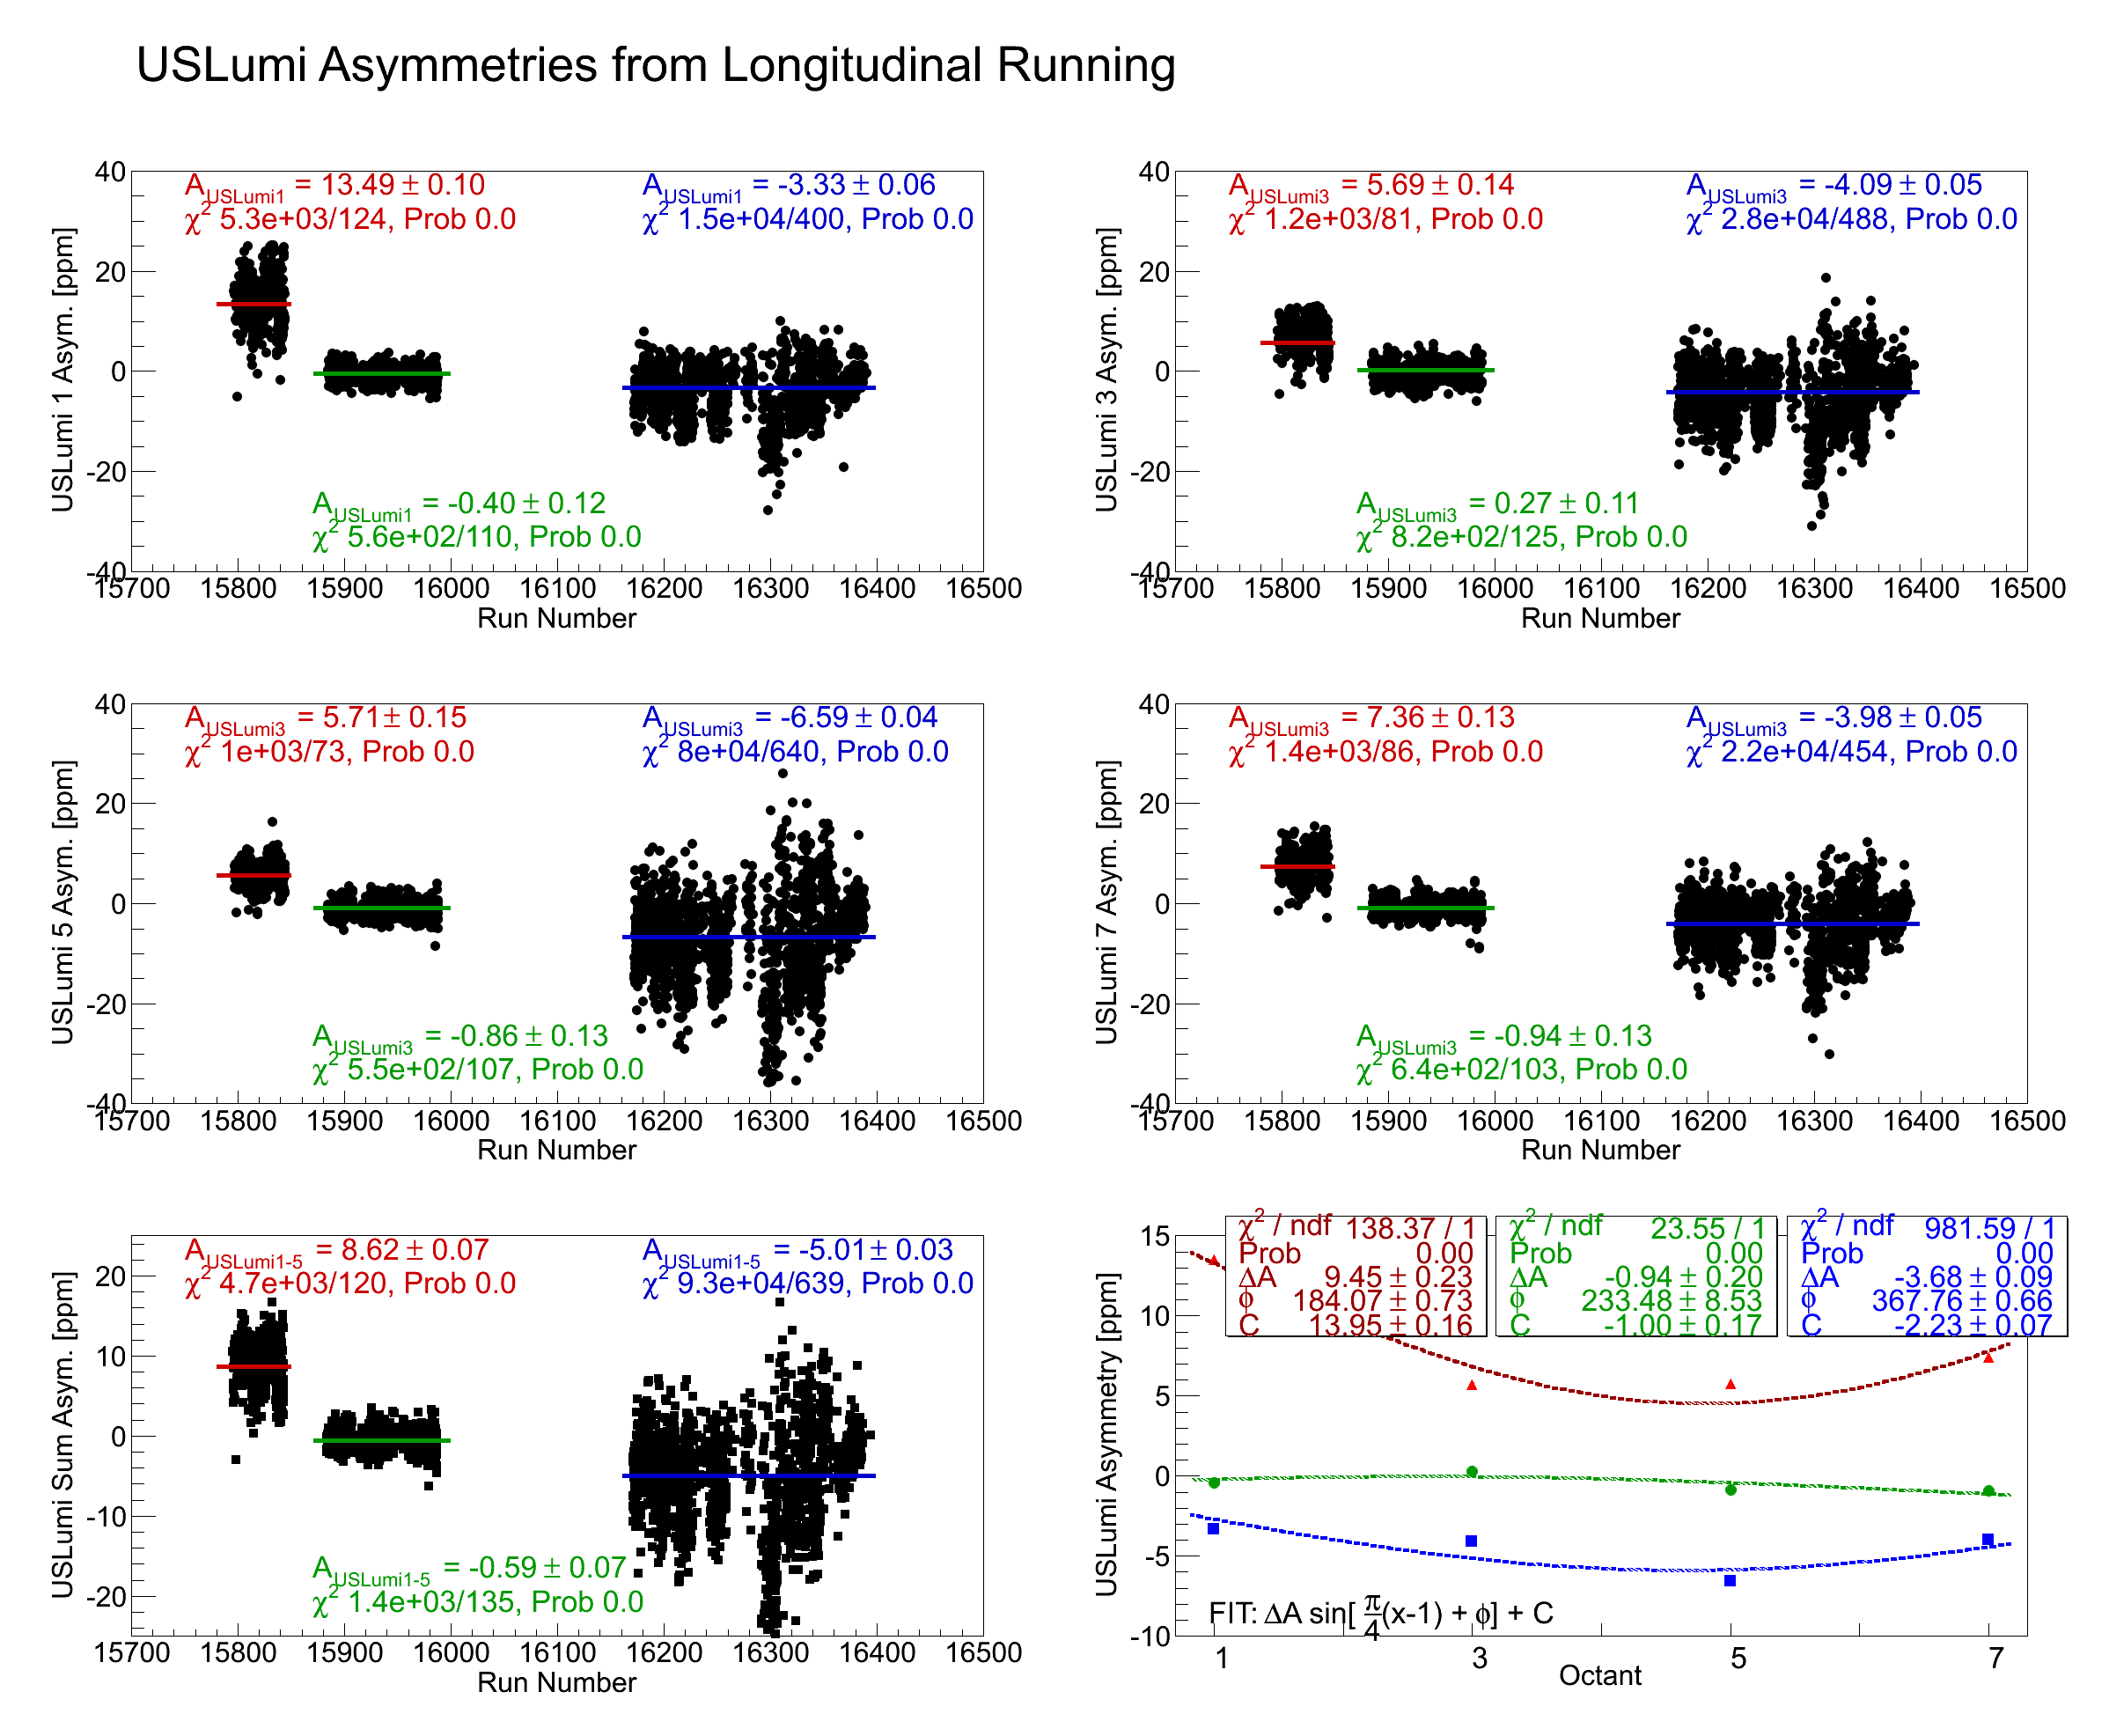
\includegraphics[width=15.0cm]{figures/USLumiSumAsymLongitudinal}
%	\end{center}
%	\caption
%	[Regressed ``5+1" USLumi asymmetries from longitudinal running.]
%	{Regressed ``5+1" USLumi asymmetries longitudinal running for octant 1, 3, 5, and 7 are shown in panel 1-4. USLumi sum asymmetry is shown in panel 5. Each point is a runlet. The average asymmetries vs octant for each time period are shown in panel 6.}
%	\label{fig:USLumiSumAsymLongitudinal}
%\end{figure}


\subsubsection{Beamline Background}
\label{Beamline Background}
%Another correction accounts for scattering sources in the beam line ($b2$). The asymmetry ($A_{b2}$) was measured, along with its dilution ($f_{b2}$), by blocking two of the eight openings in the first of the three Pb collimators with tungsten. The measured asymmetry in the blocked octants detectors was correlated with different background detectors located outside the acceptance of the main detectors for scaling during the primary measurement, assuming a constant dilution~\cite{elog:kent_analysis782}. The variation of upstream luminosity monitor asymmetry with octant during longitudinal running can provide a good indication of the beamline scattering asymmetry. The maximum variation before and after the transverse data collection period (during longitudinal running) $\Delta A_{\rm USLumi}$ = 3.534~$\pm$~0.16~ppm (Figure~\ref{fig:USLumiSumAsymLongitudinal}) was used to estimate the beamline scattering asymmetry. A very simple postulate was considered: that measured main detector asymmetry has a background with a fixed fraction and an asymmetry that scales linearly with that measured in the background monitors and USLumis. The scale factor was measured directly, correlating the MD asymmetry to background asymmetries, and was estimated to be 0.0085~$\pm$~0.0016~\cite{elog:manolis_analysis1191} from longitudinal period. The signal drops by an order of magnitude lower for inelastic scattering compared to elastic, whereas beamline background remains similar. Hence an additional factor of 10 was multiplied to incorporate the signal drop. The beamline background does not depend on polarization and is not corrected for it. Then, asymmetry for beam line scattering is given by $A_{b2}$ = $\Delta A_{\rm USLumi}\times 0.085$ = 0.300~$\pm$~0.058~ppm. 

The beamline background correction is a polarization-independent mechanical asymmetry which should be lumped with linear regression corrections~\cite{mack_QweakBackgroundCorrections}. The beamline scattering produces light in the detectors and there is a contribution to the dilution. 
The beamline background dilution factor for inelastic running is an order of magnitude larger than in the elastic kinematic setting. The total rate at the inelastic peak drops to 10\% of the total rate at the elastic peak, whereas the number of events originating in the beamline remains similar. The measured dilution for inelastic beamline scattering is 0.018~$\pm$~0.001~\cite{leacock_qweak, elog:mack_analysis784}. A 50\% uncertainty on the dilution was assigned to allow the sinusoidal modulation specific to the BNSSA. The beamline scattering dilution used for the background correction is $f_{BB}$ = 0.018~$\pm$~0.009. 
%The correction to the physics asymmetry due to beam line scattering is $c_{b2}$ = $\kappa PA_{b2}f_{b2}$ = 0.025~ppm.

\subsubsection{Other Neutral Background}
\label{Other Neutral Background}
An additional correction was applied to include soft neutral backgrounds arising from secondary interactions of scattered electrons in the scattered electron transport line, and was not accounted in the blocked octant studies~\cite{elog:mack_analysis714}. 
%A dedicated M{\o}ller~\cite{elog:buddhini_analysis553} asymmetry was measured with 0.877 GeV transverse electron beam as $A_{M{\o}ller}$ = 9.33~$\pm$~0.54~ppm. This measurement is used for the current analysis at 1.155~GeV to give an upper bound on the asymmetry. If the primary electron interaction at scraping is dominated by M{\o}ller scattering then the expected neutral asymmetry can be obtained as $A_{b3}$ = $A_{M} - A_{M{\o}ller}$ = 4.235~$\pm$~0.706~ppm.
%The primary electron interaction at scraping is partially coming from M{\o}ller scattering, but the source of the asymmetry is not well understood.
This can arise from M{\o}ller scattering, electron-proton elastic scattering, etc. Simulations are in progress~\cite{presentation:marty_2072}.
%The asymmetry from M{\o}ller scattering has a similar size but opposite sign compared to the measured transverse asymmetry~\cite{elog:buddhini_analysis553}.
The other neutral background asymmetry could be as large as 5 ppm (size of the transverse asymmetry).
To make the sign of the asymmetry uncertain, the asymmetry for other neutral background was assumed to be $B_{QTor}$ = 0.000~$\pm$~10.000~ppm. Here, uncertainty of 100\% of the measured transverse asymmetry was assigned to give an upper bound on the neutral background asymmetry. 

The neutral background dilution for the inelastic scattering has been measured as $f_{\rm neutral}$ = 0.0520~$\pm$~0.0040~(stat)~$\pm$~0.0014~(sys)~\cite{rakitha_neutral_background}. The dilution for the other neutral background was obtained by subtracting the blocked octant background from the total neutral background measured by the main detector and is given by $f_{QTor}$ = $f_{\rm neutral} - f_{BB}$ = 0.034~$\pm$~0.010. 

The correction to the physics asymmetry due to other neutral background is $c_{QTor}$ = $M_{total}B_{QTor}$ $f_{QTor}$/(1-$f_{total}$) = 0.000~$\pm$~1.616~ppm.

%Kent Paschke request: assume QTOR channel asymmetry is dominated by Moellers rather than elastics, hence change A = -0.2 to 0.0. The asymmetry increased by 2 ppb. The systematic error changed in the last digit. The correction is made properly but in the "somewhat orthogonalized list of corrections" in the output file, the quantity f2*A2/(1-ftotal) is used and is zero since A2 = 0. The 2 ppb correction mentioned above comes thru the dilution factor in the denominator of (Amsr/P)/(1-f). Gonna have to work on the "somewhat" in that summary of corrections. 

\begin{figure}[!h]
	\begin{center}
	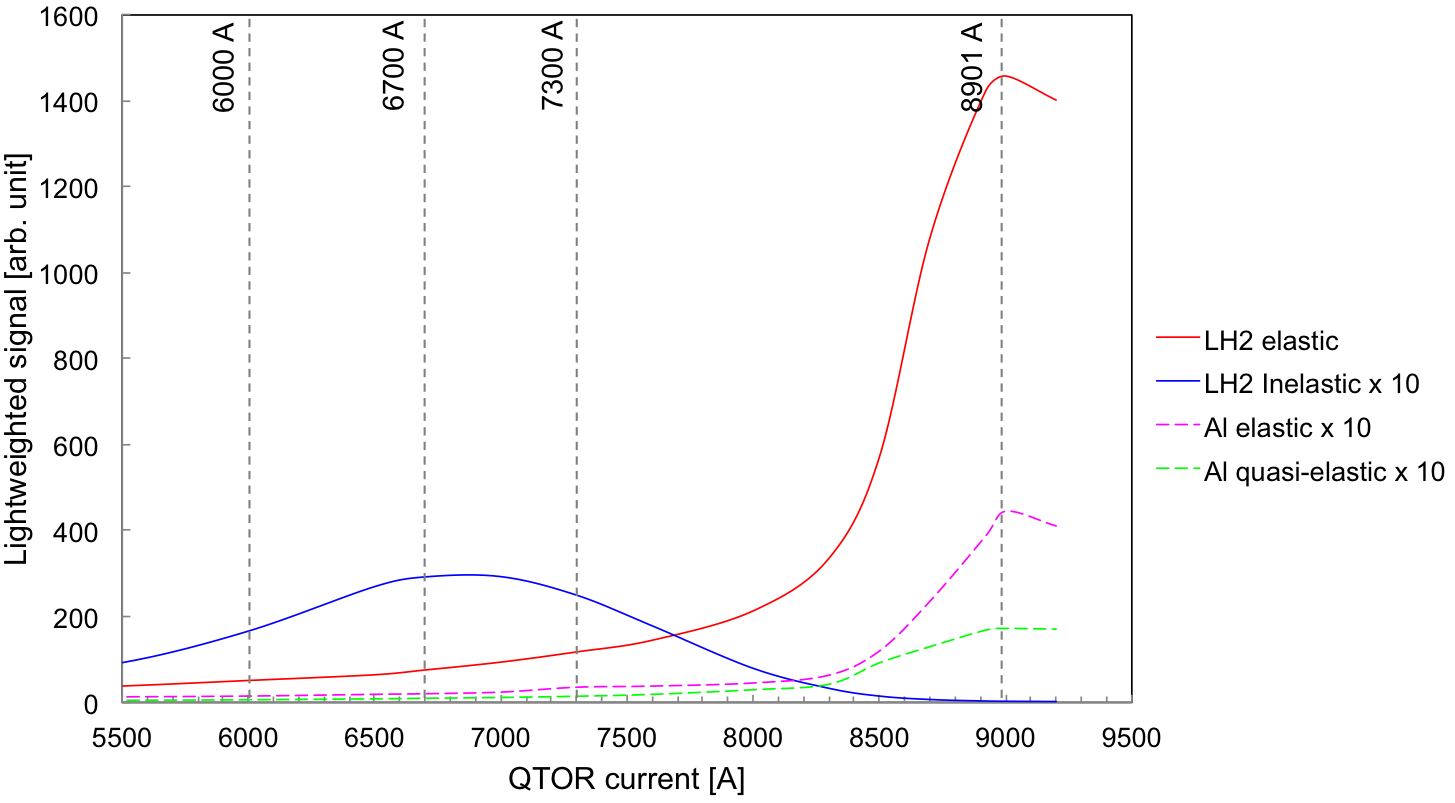
\includegraphics[width=15.0cm]{figures/qtorScan}
	\end{center}
	\caption
%	[Simulation of contributions from elastic and inelastic electron-proton and elastic electron-Al scattering from upstream and downstream target windows.]
	{
	%Inelastic transverse data set. Vertical transverse are shown in parenthesis, rest are for horizontal transverse. Number of runs in each settings are shown on top panel. Each point corresponds to $\sim$1~hour of data. LH$_{2}$ runs are shown in blue square points, 4\% downstream aluminum (Al) alloy targets are shown in purple circles, and runs with Carbon target are shown in orange diamond points. The simulated curves are from GEANT 3 simulation~\cite{elog:adesh_analysis837}. The simulated curves for LH$_{2}$ inelastic, Al elastic, and Al quasi elastic were multiplied by a factor of 10 for better visualization.
Simulation of contributions from elastic and inelastic electron-proton, and elastic electron-Al scattering from upstream (US) and downstream (DS) target windows~\cite{elog:adesh_analysis837}. All but elastic electron-proton events have been multiplied by 10 for better visualization.}
	\label{fig:qtorScan}
\end{figure}


\subsubsection{Elastic Radiative Tail}
\label{Elastic Radiative Tail}
The largest background correction comes from the elastic radiative tail ($b4$). The polarization corrected measured elastic transverse asymmetry was $B_{T}^{el}$ = -5.345~$\pm$~0.067~(stat)~$\pm$~0.076~(sys)~ppm~\cite{presentation:BPWQweakTransverse_02_21_14}. The elastic physics asymmetry from the LH$_{2}$-cell is similar in magnitude to the inelastic asymmetry but has the opposite sign.
The elastic asymmetry was measured at $Q_{el}^{2}$ = 0.0250~$\pm$~0.0006~(GeV/c)$^{2}$~\cite{PhysRevLett.111.141803} where as inelastic measurement was at $Q_{in}^{2}$ = 0.0209~$\pm$~0.0005~(GeV/c)$^{2}$ (shown in Figure~\ref{fig:inelastic_Q2}), hence it is necessary to scale it to the inelastic peak. The transverse asymmetry is proportional to $\sqrt{Q^{2}}$~\cite{PhysRevC.72.034602, PhysRevC.77.044606}. The polarization and $\sqrt{Q^{2}}$ corrected elastic asymmetry is given by $B_{el}$ = $\sqrt{\frac{Q_{in}^{2}}{Q_{el}^{2}}}B_{T}^{el}$ = -4.885~$\pm$~0.093~ppm.

As $\sim$70\% of the total signal in the inelastic peak was from elastic radiative tail (Figure~\ref{fig:qtorScan}), it was important to tackle it carefully. 
A GEANT simulation was used to extract elastic dilution. Dedicated measurements were taken at both sides of the inelastic peak (at QTor current 6000~A and 7300~A) to check the simulation. A $\sim$10\% discrepancy was observed between current mode data and GEANT simulated signal at the inelastic peak, as shown in Figure~\ref{fig:elasticDilutionDiscrepancy}. In order to incorporate this discrepancy, a 10\% systematic uncertainty was assigned to the elastic dilution for this preliminary analysis. A more detailed simulation is ongoing to explore this difference. The signal size for inelastic transverse is $\sim$2-3 times smaller than that of the elastic signal. Although the signal reduces for inelastic, the nonlinearity in the detector remains the same and might be responsible for this discrepancy.
The simulated elastic dilution factor is given by $f_{el}$ = 0.701~$\pm$~0.070~\cite{elog:adesh_analysis837, elog:nur_ancillary59}. 

The correction to the physics asymmetry due to the elastic radiative tail is $c_{el}$ = $M_{total}B_{el}f_{el}/(1-f_{total})$ = -17.063~$\pm$7.304~ppm.


\begin{figure}[!h]
	\begin{center}
	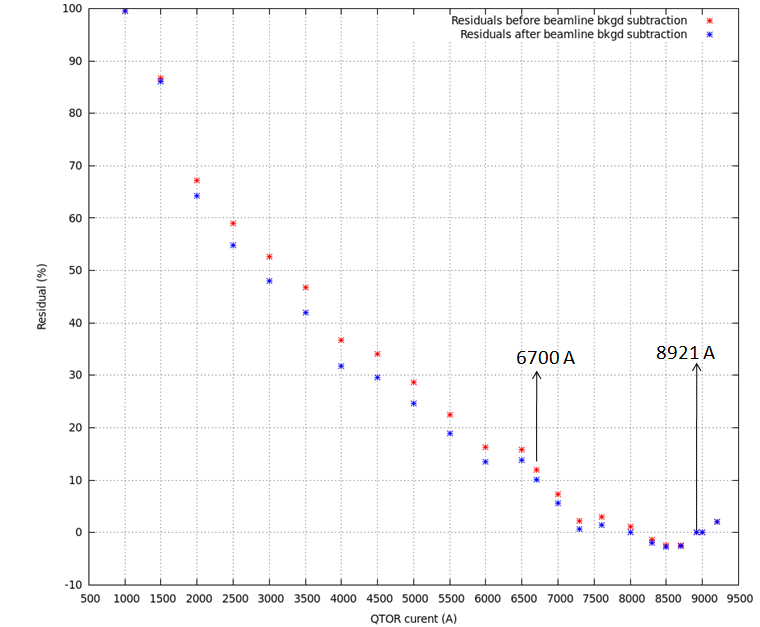
\includegraphics[width=15.0cm]{figures/elasticDilutionDiscrepancy}
	\end{center}
	\caption
%	[The residual of yield using Data and simulation from GEANT 3.]
	{The residual of yield using Data and simulation from GEANT 3~\cite{elog:adesh_analysis837} are shown in the figure. A $\sim$10\% discrepancy was observed at inelastic peak (6700~A) between data and simulation for matching them at elastic peak (8921~A). Beamline background correction to the yield did not improve the discrepancy. }
	\label{fig:elasticDilutionDiscrepancy}
\end{figure}

\begin{figure}[!h]
	\begin{center}
	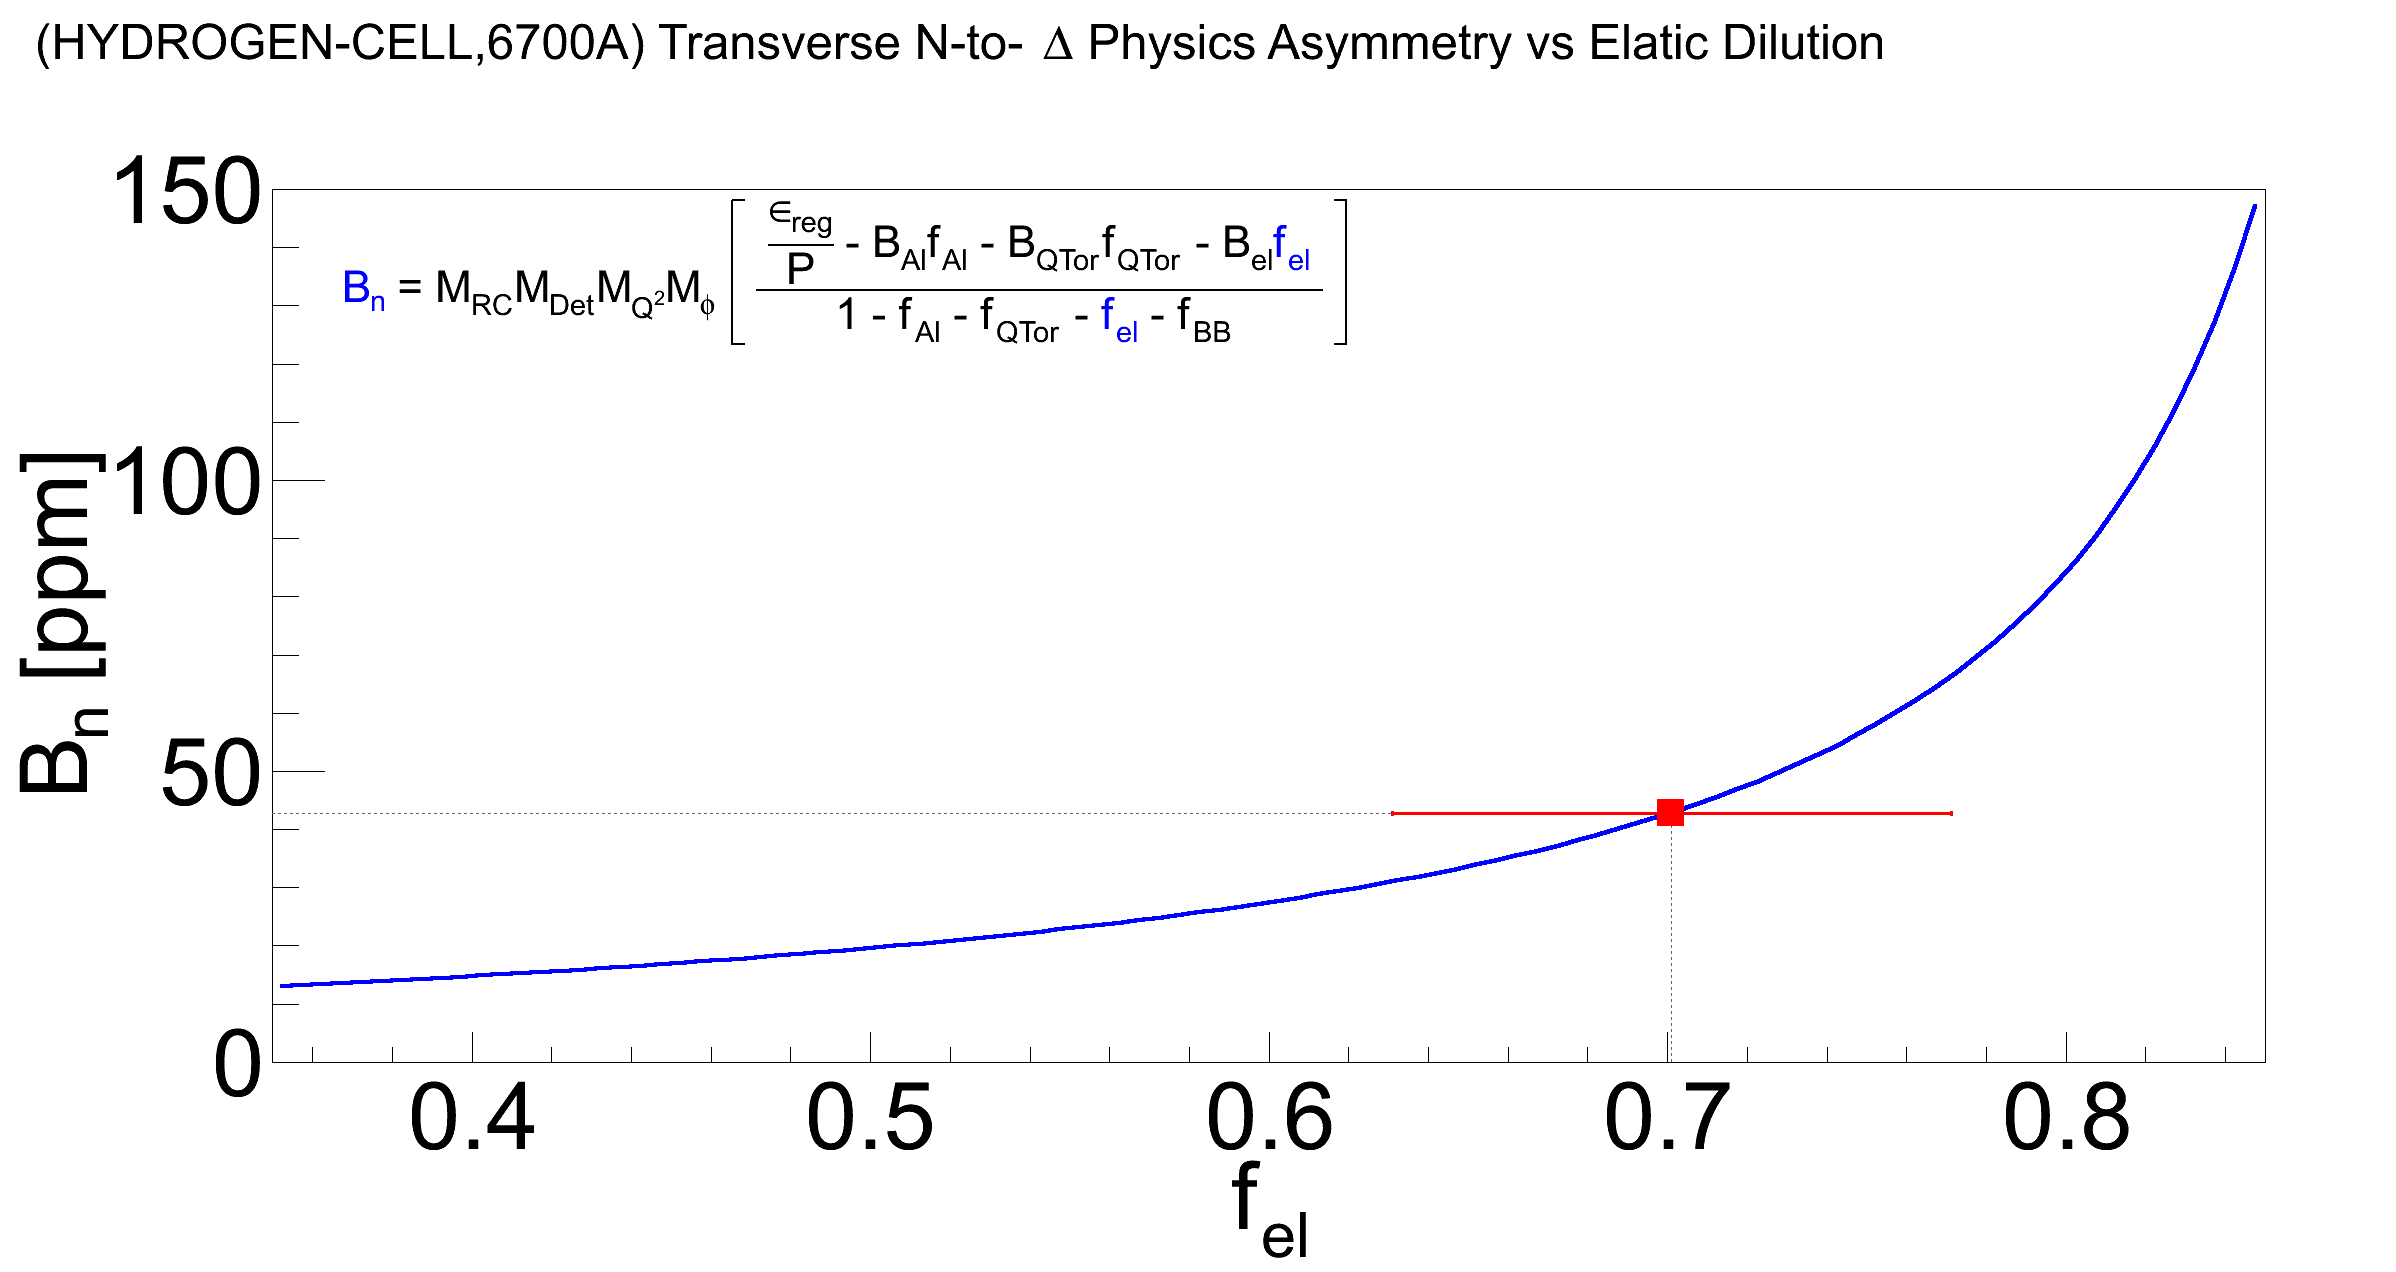
\includegraphics[width=15.0cm]{figures/asymVsElDilutionLH2}
	\end{center}
	\caption
%	[The variation of beam normal single spin asymmetry with elastic dilution.]
	{The variation of beam normal single spin asymmetry with elastic dilution.}
	\label{fig:asymVsElDilutionLH2}
\end{figure}


\subsection{Other Corrections}
\label{Other Corrections}
Another set of corrections is used to remove all the experimental bias from the measured asymmetry before extracting BNSSA. The measured asymmetry is corrected for the electromagnetic (EM) radiative corrections, light weighting on the \v{C}erenkov detector, and $Q^{2}$ precision. These corrections are considered as independent factors and are applied to the measured asymmetry.

%Electromagnetic (EM) radiation causes energy loss and depolarization [154] of the electrons. To extract the beam normal single spin asymmetry at the effective $Q^{2}$ and beam polarization, the measured $A_{N}$ needs to be corrected for these EM radiative effects. The deduced radiative correction for elastic e+p scattering from simulations with and without bremsstrahlung, using methods described in Refs.~\cite{PhysRevLett.82.1096, PhysRevC.69.065501} was found to be $M_{RC}$ = 1.010~$\pm$~0.005. The same radiative correction was used for this dataset.
%$M_{Det}$ = 1.000~$\pm$~0.000 accounts for the measured light variation and nonuniform $Q^{2}$ distribution across the detector bars. $M_{Bin}$ = 1.000~$\pm$~0.000 is an effective kinematics correction~\cite{PhysRevC.69.065501} that corrects the asymmetry from $\langle A(Q^{2})\rangle$ to $A(\langle Q^{2}\rangle)$, and $M_{Q^{2}}$ = 1.000~$\pm$~0.030 represents the precision in calibrating the central $Q^{2}$.


\subsubsection{Radiative Correction}
\label{Radiative Correction}
The energy loss and depolarization of the electrons is a result of electromagnetic (EM) radiation~\cite{PhysRev.114.887}. The measured asymmetry needs to be corrected for these EM radiative effects to obtain the beam normal single spin asymmetry at the effective $Q^{2}$ and beam polarization. The deduced radiative correction for elastic electron-proton scattering from simulations with and without bremsstrahlung, using methods described in Refs.~\cite{PhysRevLett.82.1096, PhysRevC.69.065501}, was found to be $M_{RC}$ = 1.010~$\pm$~0.010~\cite{buddhini_qweak}. The same radiative correction was used for this data set as there were no existing simulations available for inelastic electron-proton scattering. This correction does not have a significant impact in the final asymmetry, hence it was not unreasonable to use the existing elastic simulation result. %A uncertainty of 100\% is assigned on the radiative correction.

%$M_{RC}$ = $M_{EB}\times M_{IB}\times M_{depolarization}$

\subsubsection{Detector Bias Correction}
\label{Detector Bias Correction}

The correction between light yield and $Q^{2}$ across the detector bars affects the measured asymmetry and needs to be accounted for in the final BNSSA extraction. The multiplicative correction factor to be applied to the data is 

\begin{equation} \label{equ:eqQ2Acceptance1}
M_{Det} = \frac{\epsilon_{\rm no-bias}^{\rm sim}}{\epsilon_{\rm bias}^{{\rm sim}}} = \sqrt{\frac{(Q^{2})_{\rm no-bias}^{\rm sim}}{(Q^{2})_{\rm bias}^{\rm sim}} }.
\end{equation}

Here, $\epsilon^{\rm sim}_{\rm bias}$ and $\epsilon^{\rm sim}_{\rm no-bias}$ are the simulated asymmetries with and without light-collection bias, respectively.
The detector bias correction used for this analysis is $M_{Det}$ = 0.998~$\pm$~0.002 and is obtained using transverse simulation results~\cite{elog:peiqing_analysis589, buddhini_qweak}.

\begin{figure}[!h]
	\begin{center}
	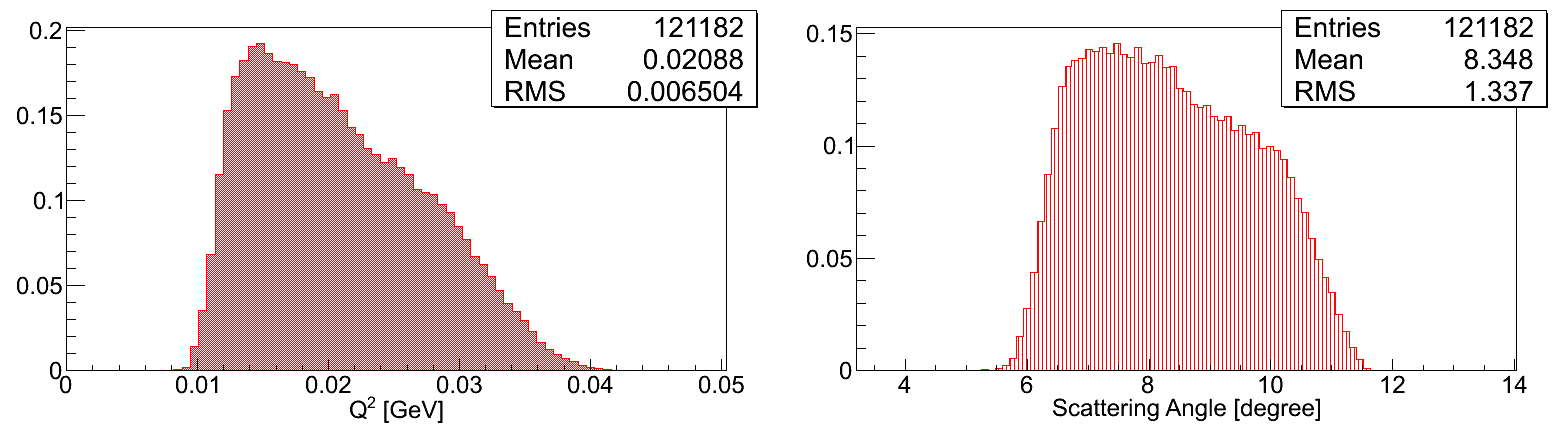
\includegraphics[width=15.0cm]{figures/inelastic_Q2}
	\end{center}
	\caption
%	[The $Q^{2}$ from GEANT 3 simulation.]
	{The $Q^{2}$ from GEANT 3 simulation~\cite{elog:nur_ancillary44}. The $Q^{2}$ was weighted by cross section and did not include any internal bremsstrahlung in the simulation (left panel). The simulated scattering angle is also shown in the right panel.}
	\label{fig:inelastic_Q2}
\end{figure}

\subsubsection{$Q^{2}$ Precision}
\label{Q2 Precision}

The $Q^{2}$ for inelastic electron-proton scattering was determined using GEANT 3 simulation and was found to be 0.0209~$\pm$~0.0005~(GeV/c)$^{2}$~\cite{elog:nur_ancillary44}, as shown in Figure~\ref{fig:inelastic_Q2}. Internal bremsstrahlung was not included in the simulation. The simulation was benchmarked by the tracking mode experimental data to represent the geometry of the experimental setup, collimation, and magnetic spectrometer.
The cross section weighted $Q^{2}$ was simulated at main detector using the reaction $e + p \rightarrow e + n + \pi^{+}$~\cite{elog:nur_ancillary44}. The two-body scattering process, and energy and momentum conservation were used to do the calculation. The scattered electron energy, and $Q^{2}$ are expressed as 
%$E^{\prime} = RANDOM()\times(E_{in} - M_{e}) + M_{e}$ $Q_{2} = 4EE^{\prime}sin^{2}\theta$

\begin{equation} \label{equ:eqQ2Calculation}
\begin{split}
E^{\prime} &= RANDOM()\times(E_{in} - M_{e}) + M_{e} \\
Q^{2} &= 4EE^{\prime}\sin^{2}\theta,
\end{split}
\end{equation}

\noindent 
where $E_{in}$ is the incident beam, $M_{e}$ is electron mass, and $\theta$ is scattering angle. 
%A 2.0\% run to run variation of $Q^{2}$ was seen from the tracking data and added as systematic uncertainty in $Q^{2}$ estimation. 
It was important to propagate the precision of $Q^{2}$ in the final physics asymmetry. Based on theory~\cite{Afanasev200448}, the transverse beam spin asymmetries $A_{N}$ at low $Q^{2}$ behave like

\begin{equation} \label{equ:eqQ2Acceptance1}
B_{n} \approx \sqrt{Q^{2}} = m\sqrt{Q^{2}}.
\end{equation}

\begin{equation} \label{equ:eqQ2Acceptance2}
dB_{n} = \pm \frac{1}{2} \frac{m}{\sqrt{Q^{2}}} dQ^{2}
= \pm \frac{1}{2} \frac{34.7}{\sqrt{0.02078}} 0.0005
=  0.0601~\text{ppm}.
\end{equation}

Using Equation~\ref{equ:eqQ2Acceptance1} on $Q^{2}$ and a 5~ppm measured asymmetry, the proportionality constant in the above relation can be calculated as 34.7~ppm/(GeV/c). The estimated uncertainty on the measured asymmetry due to the uncertainty in determining $Q^{2}$ is 0.061~ppm (Equation~\ref{equ:eqQ2Acceptance2}). 
%This is a 1.2\% relative correction. 
A correction of $M_{Q^{2}}$ = 1.000~$\pm$~0.012 was applied to include the precision in calibrating the central value of $Q^{2}$.

%\begin{equation} \label{equ:eqQ2Acceptance2}
%\begin{split}
%dB_{n} = \pm \frac{1}{2} \frac{m}{\sqrt{Q^{2}}} dQ^{2} \\
%= \pm \frac{1}{2} \frac{31.0}{\sqrt{0.02078}} 0.0005\\
%=  0.0538 ppm
%\end{split}
%\end{equation}


%\begin{center}
%\framebox[\frameboxsize][c]{$Q2$ Acceptance is $\sim$0.0601~ppm.}
%\end{center}

\subsubsection{Azimuthal Acceptance Correction}
\label{Azimuthal Acceptance Correction}

The acceptance of a single Q-weak \v{C}erenkov detector is only 49\% of an octant (section~\ref{Q-weak Kinematics}), so the reported asymmetry from a detector is an average over 22\degrees{} azimuthal angle ($\phi$). Each detector bar measures an average asymmetry over a range of $\phi$ selected by the collimators (details in~\cite{buddhini_qweak, elog:birchall_analysis373}). The effect of averaging cosines for a variable of the form $y(\phi) = \epsilon\cos(\phi + \delta)$ over the azimuthal angle yields 

\begin{equation} \label{equ:eqDetectorNonlinearity}
AVG[y(\phi)] = \frac{ \epsilon\int_{\phi_{0}-\Delta\phi}^{\phi_{0}+\Delta\phi} \cos(\phi+\delta)\,\mathrm{d}\phi }{(\phi_{0}+\Delta\phi)-(\phi_{0}-\Delta\phi)} = \epsilon\cos (\phi_{0} + \delta) \times \frac{\sin\Delta\phi}{\Delta\phi}, 
\end{equation}

\noindent
where $\phi_{0}$ is the nominal azimuthal location of the detector with $\Delta\phi$ coverage. Similarly, for sines, $AVG[y(\phi)] = \epsilon\sin (\phi_{0} + \delta) \times \frac{\sin\Delta\phi}{\Delta\phi}$. So the measured asymmetry from each detector needs to be scaled by a factor of $M_{\phi}$ = 1/$\frac{\sin\Delta\phi}{\Delta\phi}$ to correct for the acceptance\footnote{Here, the collimator is assumed to remove 49\% of the octant acceptance (i.e 49\% of 45\degrees{})}. $\Delta\phi$ = 11.025\degrees{} yields the scale factor to be $M_{\phi}$ = 1/0.9938 = 1.006~$\pm$~0.006.
% implies the amplitude from the transverse fits to the octant asymmetries should be scaled by a factor of $\frac{\sin\Delta\phi}{\Delta\phi}$ = 0.9938. 
%The detector acceptance corrected measured asymmetry can be extracted as
%\begin{equation} \label{equ:asymmetryDetAcptCorrected}
%\epsilon_{M}^{\rm in} = \frac{\epsilon_{M}}{0.9938} = 5.127~\text{ppm}.
%\end{equation}
%A conservative 100\% uncertainty was used for $\Delta\phi$, which yields a systematic uncertainty of 0.004 in the correction.
A conservative 100\% uncertainty was used for the correction.

\subsection{Beam Normal Single Spin Asymmetry in LH$_{2}$}
Summary of required quantities to extract the beam normal single spin asymmetry from the transverse data set presented so far using

%\begin{equation} \label{equ:PhysicsAsymmetry}
%B_{n} = M_{RC}M_{Det}M_{Q^{2}}M_{\phi} \left[ \frac{\left(\frac{A^{in}_{M}}{P}\right) - A_{b1}f_{b1} - A_{b2}f_{b2} - A_{b3}f_{b3} - A_{b4}f_{b4} }{1 - f_{b1} - f_{b2} - f_{b3} - f_{b4}} \right] 
%\end{equation}
\begin{equation} \label{equ:PhysicsAsymmetry}
B_{n} = M_{RC}M_{Det}M_{Q^{2}}M_{\phi} \left[ \frac{\left(\frac{\epsilon_{reg}}{P}\right) - B_{Al}f_{Al} - B_{QTor}f_{QTor} - B_{el}f_{el} }{1 - f_{Al} - f_{BB} - f_{QTor} - f_{el}} \right] 
\end{equation}
is shown in Table~\ref{tab:PhysicsAsymInput}. Equation~\ref{equ:PhysicsAsymmetryShort} has been expanded to obtain Equation~\ref{equ:PhysicsAsymmetry}. 
%The input quantities for Equation~\ref{equ:PhysicsAsymmetry} are summarized in the Table~\ref{tab:PhysicsAsymInput}.
Using all the input values in Equation~\ref{equ:PhysicsAsymmetry} gives the beam normal single spin asymmetry in inelastic electron-proton scattering

\begin{table}[!h]
\begin{center}
  	\caption
%  	[Summary of input quantities to extract the BNSSA.]
  	{Summary of input quantities to extract the BNSSA. The measured regressed asymmetry is corrected for detector acceptance using the factor provided in the table. The table shows the contributions of normalization factors on $\epsilon_{reg}$, then the properly normalized contributions from other sources. Background corrections listed here include $M_{\rm total}B_{bi}f_{bi}/(1-f_{total})$. Uncertainties in BNSSA due to dilution fraction and background asymmetry uncertainties are noted separately.
  	}
  \begin{tabular}{ l | c | c | c }
%    \hline
    \noalign{\hrule height 1pt}
    \multicolumn{4}{c}{Input parameters} \\
    \hline    
    Measured asymmetry ($\epsilon_{reg}$)	&	\multicolumn{3}{l}{5.095 $\pm$ 0.455~ppm}  \\
    Beam polarization		(P)			&	\multicolumn{3}{l}{0.875 $\pm$ 0.008} \\
%    Detector acceptance correction		&	\multicolumn{3}{l}{0.9938} \\
%	  \hline 
    \noalign{\hrule height 1pt}
    \multicolumn{4}{c}{Background corrections} \\
    \hline
    \multirow{3}{*}{Quantity} &	Asymmetry & Dilution & Correction \\
    &	($B_{bi}$) & ($f_{bi}$) & $c_{bi}= B_{bi}f_{bi}/(1-f_{total})$ \\
    & [ppm] &  & [ppm] \\
	\hline
	Target windows (Al) 			& 9.185 $\pm$ 1.409 		& 0.033 $\pm$ 0.002 & 1.416 $\pm$ 0.246 \\
	Other neutral bkg. (QTor)	& 0.000 $\pm$ 10.000 	& 0.034 $\pm$ 0.010 & 0.000 $\pm$ 1.616 \\
	Elastic asymmetry (el) 		& -4.885 $\pm$ 0.093		& 0.701 $\pm$ 0.070 & -17.063 $\pm$ 7.304 \\
	Beamline background (BB)		&						& 0.018 $\pm$ 0.009 &  \\
%    \hline 
    \noalign{\hrule height 1pt}
    \multicolumn{4}{c}{Other corrections} \\
    \hline
    Radiative correction ($M_{RC}$)		&	\multicolumn{3}{l}{1.010 $\pm$ 0.010} \\
    Detector bias ($M_{Det}$)					&	\multicolumn{3}{l}{0.998 $\pm$ 0.002} \\
    $Q^{2}$ acceptance ($M_{Q^{2}}$)	&	\multicolumn{3}{l}{1.000 $\pm$ 0.012} \\
	Azimuthal acceptance ($M_{\phi}$)	&	\multicolumn{3}{l}{1.006 $\pm$ 0.006} \\
%	\hline 
    \noalign{\hrule height 1pt}
  	\end{tabular}
  \label{tab:PhysicsAsymInput}
\end{center}
\end{table}

\begin{equation} \label{equ:FinalResult}
B_{n} = 42.82 \pm 2.45~\text{(stat)} \pm 16.07~\text{(sys)}~\text{ppm}
\end{equation}
for the effective kinematics of acceptance averaged electron energy $\langle E_{beam}\rangle$ = 1.155~$\pm$~0.003~GeV, $\langle Q^{2}\rangle$ = 0.0209~$\pm$~0.0005~(GeV/c)$^{2}$, an average scattering angle $\langle\theta\rangle$ = 8.3\degrees{}, and missing mass $W$~=~1.204~GeV. The contributions from the different uncertainty sources into the final measurement are summarized in Figure~\ref{fig:physicsErrorChart}. The dominant correction to the asymmetry comes from the elastic dilution tail whereas the dominant uncertainty on the measured asymmetry comes from statistics.

%The final transverse asymmetry, corrected for backgrounds and beam polarization, was found to be $B_{n}$ = 42.82 $\pm$ 2.45 (stat) $\pm$ 16.06 (sys)~ppm at beam energy $E_{beam}$ = 1.155~GeV, scattering angle $\theta$ = 8.3\degrees{}, and missing mass $W$ = 1.2~GeV.

\begin{figure}[!h]
	\begin{center}
	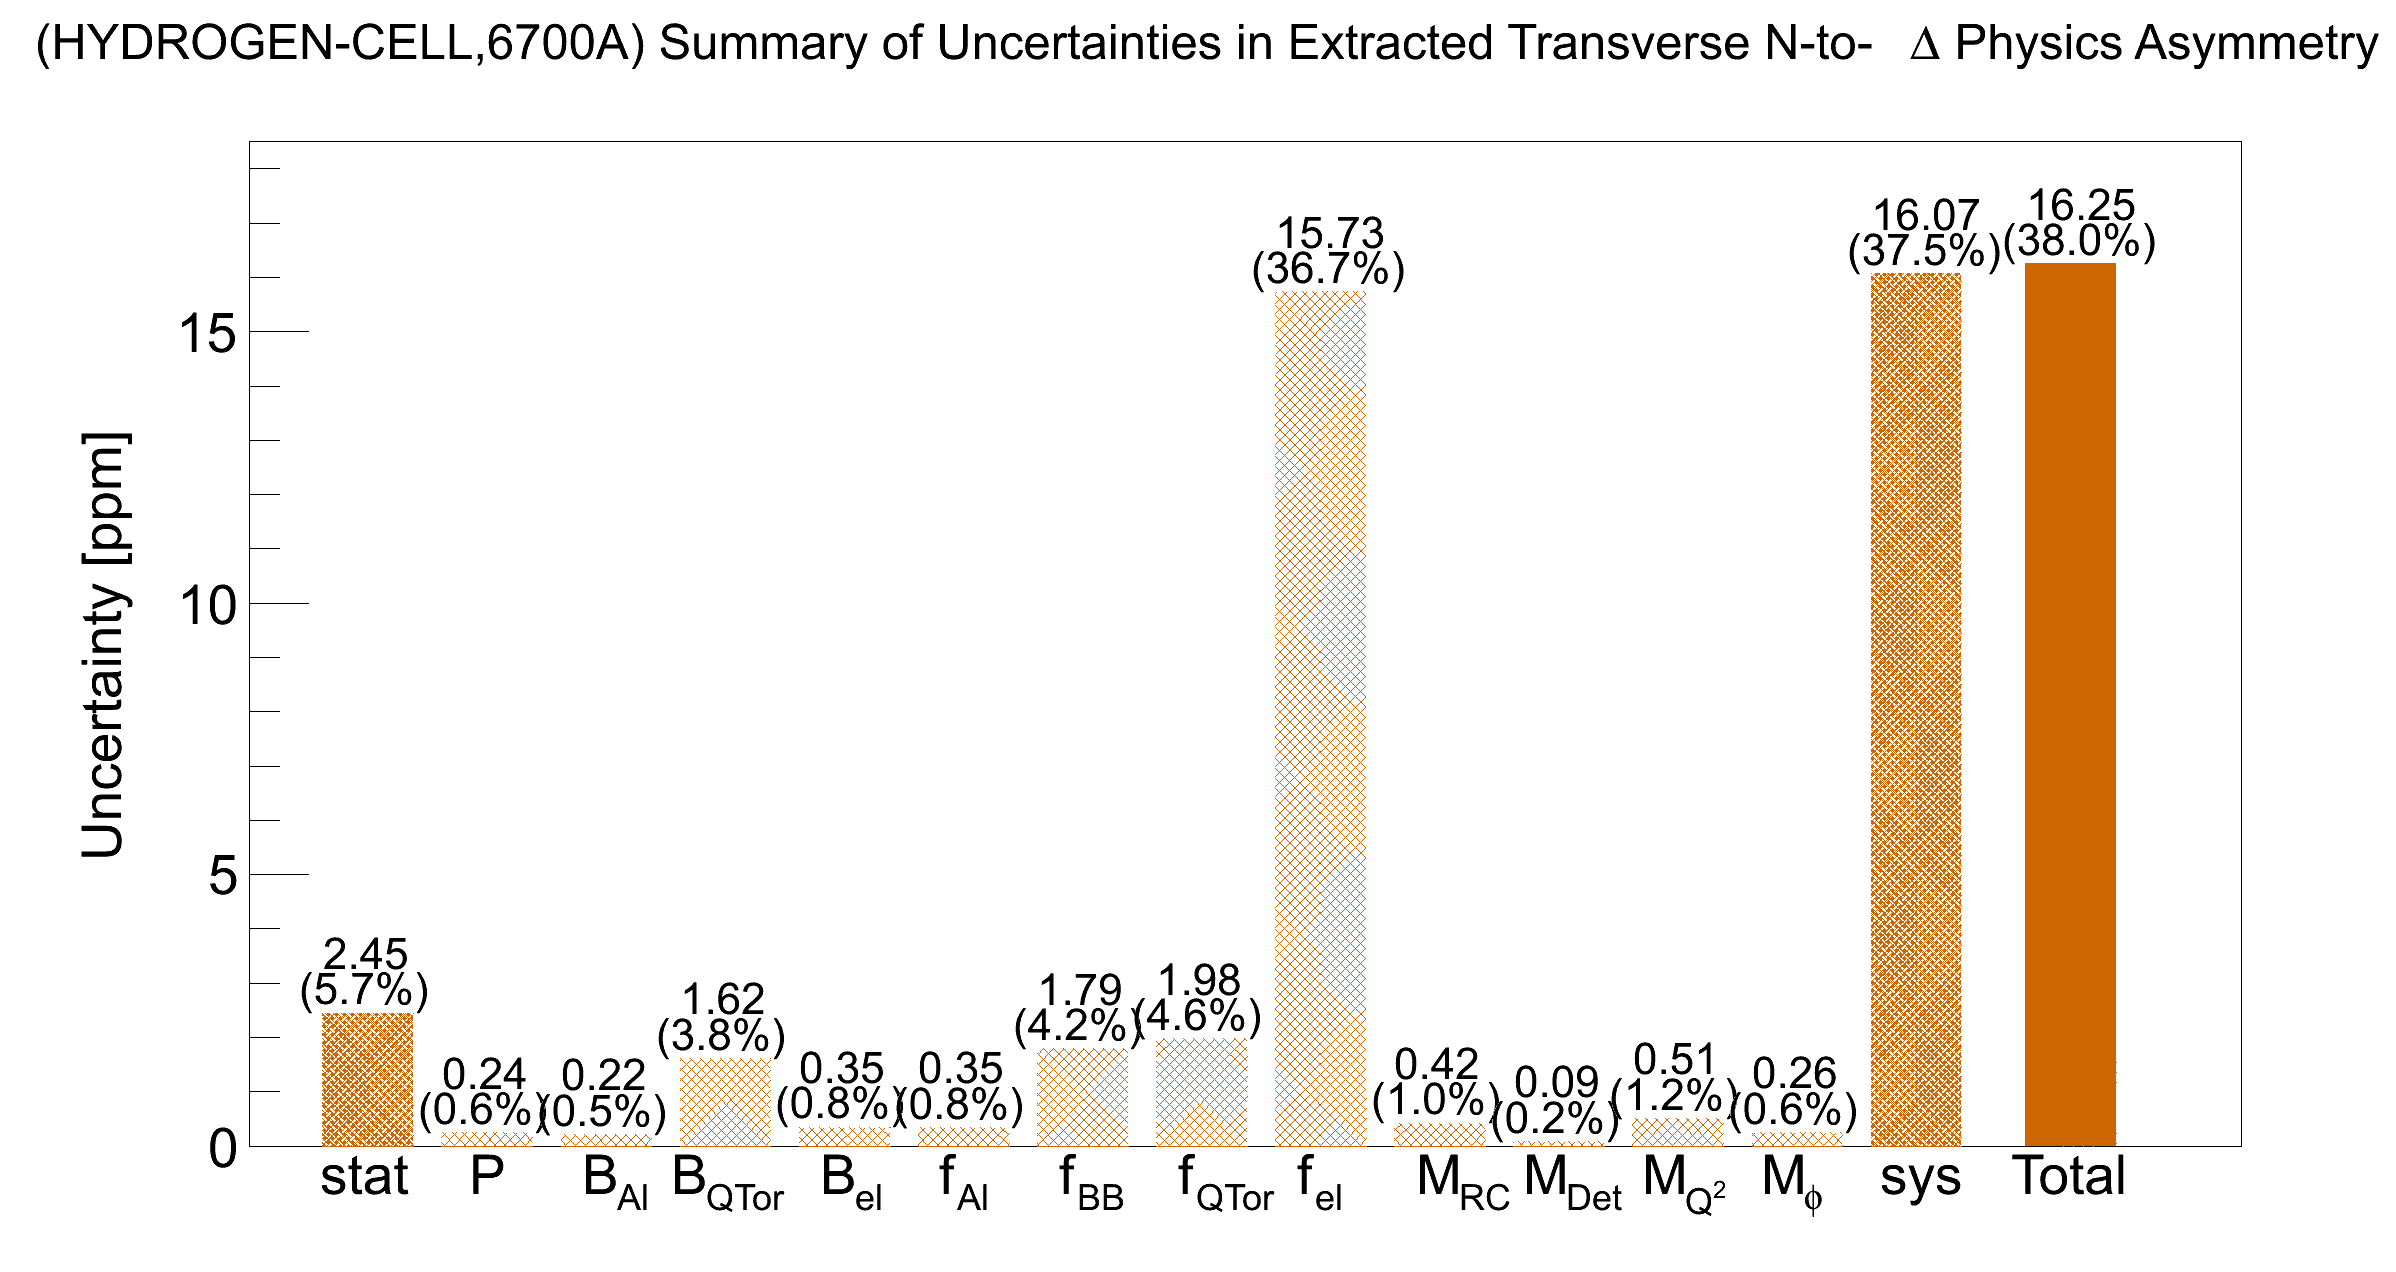
\includegraphics[width=15.0cm]{figures/physicsErrorChart}
	\end{center}
	\caption
%	[Summary of uncertainties in inelastic beam normal single spin asymmetry extraction.]
	{Summary of uncertainties in inelastic beam normal single spin asymmetry extraction. Measurement systematic contains the systematic uncertainties related to the extraction of the physics asymmetry such as regression, nonlinearity and acceptance averaging. The uncertainties are in ppm and the corresponding relative uncertainties are shown in parentheses.}
	\label{fig:physicsErrorChart}
\end{figure}


%\begin{table}[!h]
%\begin{center}
%  	\caption
%  	[Systematic error table.]
%  	{Systematic error table.}
%  \begin{tabular}{ c | c | c }
%%    \hline
%    \noalign{\hrule height 1pt}
%    \multirow{2}{*}{Uncertainty from}	&	Uncertainty	&	Relative uncertainty \\
%							&	[ppm]	&	[\%] \\
%%	\hline
%    \noalign{\hrule height 1pt}
%	$A_{M}^{in}$		&	2.36		&	5.9 \\
%	P				&	0.26		&	0.7 \\
%	$A_{b1}$			&	0.17		&	0.4 \\
%	$A_{b2}$			&	0.55		&	1.4 \\
%	$A_{b3}$			&	0.02		&	0.1 \\
%	$A_{b4}$			&	0.47		&	1.2 \\
%	$f_{b1}$			&	0.30		&	0.7 \\
%	$f_{b2}$			&	0.13		&	0.3 \\
%	$f_{b3}$			&	1.70		&	4.3 \\
%	$f_{b4}$			&	13.96	&	35.2 \\
%	$M_{RC}$			&	0.00		&	0.0 \\
%	$M_{Det}$			&	0.00		&	0.0 \\
%	$M_{Bin}$			&	0.00		&	0.0 \\
%	$M_{Q^{2}}$		&	1.19		&	3.0 \\
%%	\hline
%    \noalign{\hrule height 1pt}
%	Total					& 	14.33 	&	36.1 \\
%%    \hline
%    \noalign{\hrule height 1pt}
%  	\end{tabular}
%  \label{tab:PhysicsError}
%\end{center}
%\end{table}

%\begin{center}
%\framebox[\frameboxsize][c]{Extracted physics asymmetry $A_{N}$ = 39.71~$\pm$2.36 (stat)~$\pm$~14.33 (sys)~ppm.}
%\end{center}



%%%%%%%%%%%%%%%%%%%%%%%%%%%%%%%%%%%%%%%%%%%%%%%%%%%%%%%%%%%%%
\section{Comparison With Model Calculation}
\label{Comparison With Model Calculation}

No existing model calculation for beam normal single spin asymmetry was available at Q-weak kinematics during this analysis. Pasquini et al.~\cite{presentation:pasquini_Mainz} presented beam asymmetry in inelastic electron scattering (as shown in Figure~\ref{fig:PasquiniInelasticTransverseAsymmetryModel}, chapter~\ref{THEORY}) for large scattering angle at energies E = 0.424, 0.570, 0.855 GeV. The BNSSA were calculated separately for $\Delta$ and N intermediate states. The total asymmetry was the sum of these two intermediate states. 
Relatively large asymmetries were observed in the forward region; these are dominated by quasi Virtual Compton Scattering (VCS) kinematics where one exchanged photon becomes quasi-real.
%Large asymmetries in the forward region dominated by quasi-VCS kinematics where one exchanged photon becomes quasi-real
These asymmetries are  sensitive to $\gamma^{\ast}\Delta\Delta$ form factors and can be a unique tool to study it~\cite{Alexandrou2009115}. 

%large asymmetries in the forward region dominated by quasi-VCS kinematics where one exchanged photon becomes quasi-real~\cite{presentation:pasquini_Mainz}
%
%* large asymmetries in the forward region
%* sensitive to $\gamma^{\ast}\Delta\Delta$ form factors~\cite{Alexandrou2009115}

\begin{figure}[!h]
	\begin{center}
	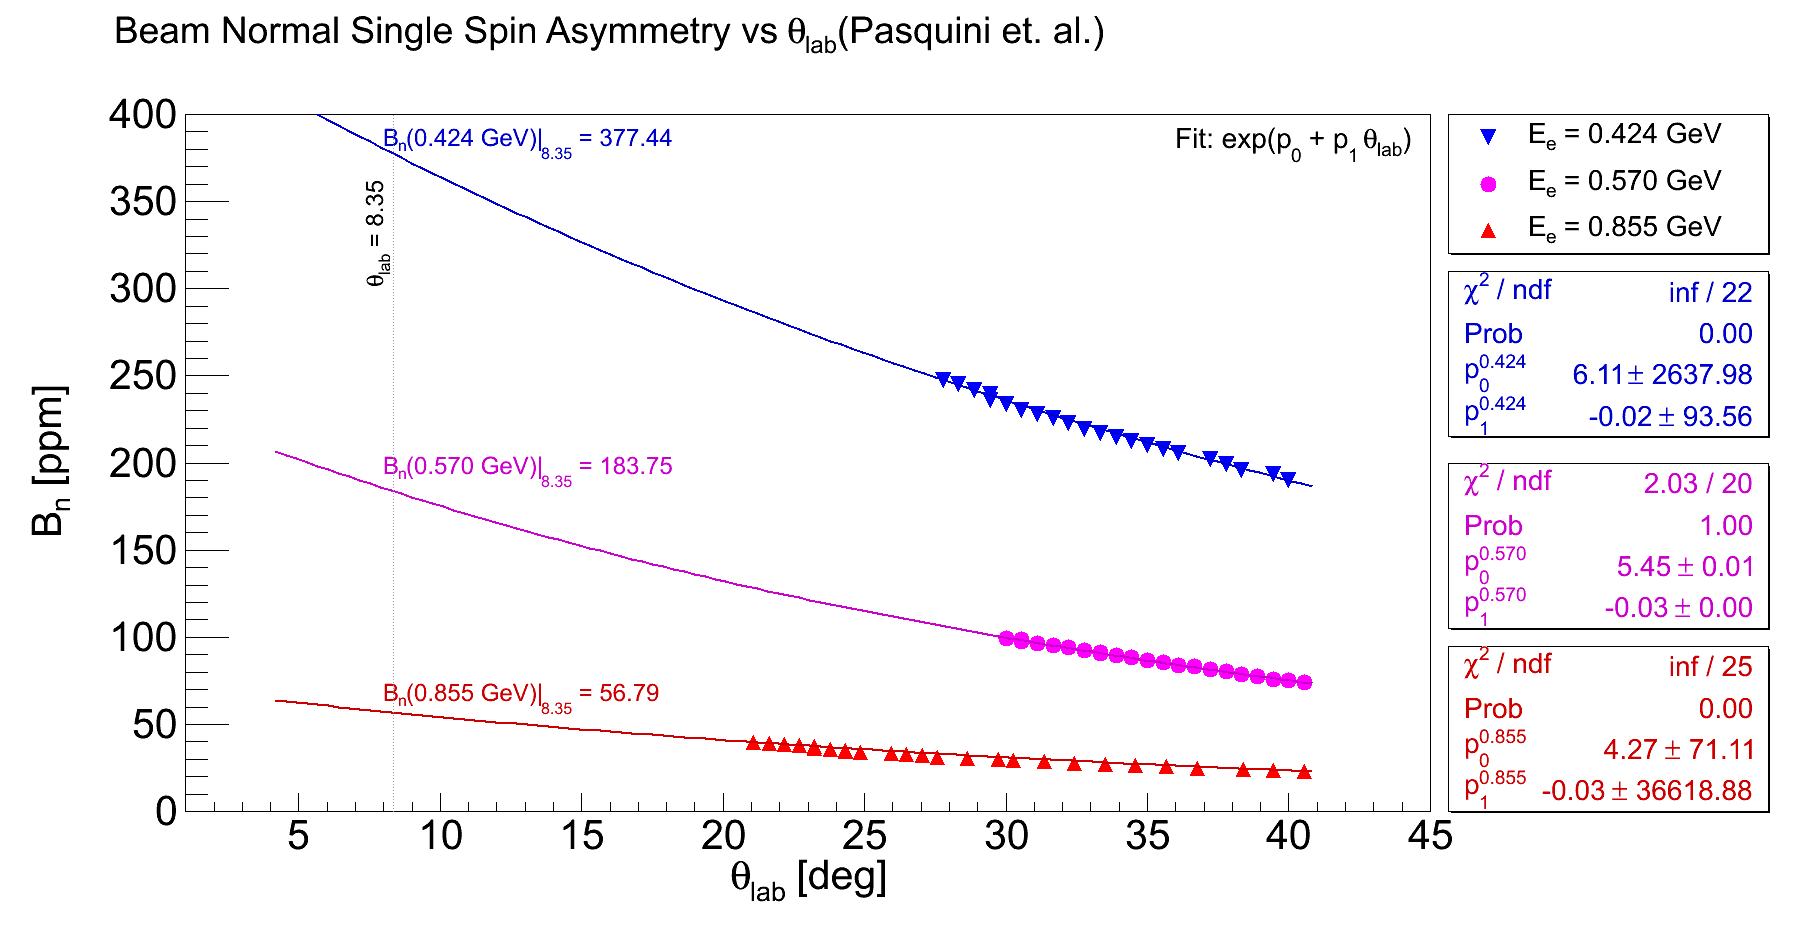
\includegraphics[width=15.0cm]{figures/theoryAsymmetryPasquini}
	\end{center}
	\caption
%	[BNSSA calculation from Pasquini et al.]
	{BNSSA calculation from Pasquini et al. The points are taken from~\cite{presentation:pasquini_Mainz}. Then, the calculation is fitted with a function of the form $f(\theta_{\rm lab}) = exp(p_{0}+p_{1}\theta_{\rm lab})$ and extrapolated to Q-weak $\theta_{\rm lab}$ value. }
	\label{fig:theoryAsymmetryPasquini}
\end{figure}

These asymmetries were extrapolated to forward angle down to $\theta_{\rm lab}\textless$5\degrees{} using a suitable fit for all available three energies from~\cite{presentation:pasquini_Mainz}, as shown in Figure~\ref{fig:theoryAsymmetryPasquini}. The asymmetries were obtained at $\theta_{\rm lab}$ = 8.35\degrees{} for three energies and extrapolated to Q-weak energy $E_{beam}$ = 1.155 GeV in Figure~\ref{fig:theoryAsymmetryPasquiniEnergyDependence}. Using this hand waving toy model, the obtained BNSSA is $B_{n}[{\rm model}]$ = 12.15~ppm at Q-weak kinematics. The asymmetry from this analysis, $B_{n}[{\rm Q-weak}]$ = 42.82~$\pm$~16.25~ppm is also shown in the Figure~\ref{fig:theoryAsymmetryPasquiniEnergyDependence}. The extrapolation uncertainties are large but can not be realistically estimated. New calculation are in progress. 

\begin{figure}[!h]
	\begin{center}
	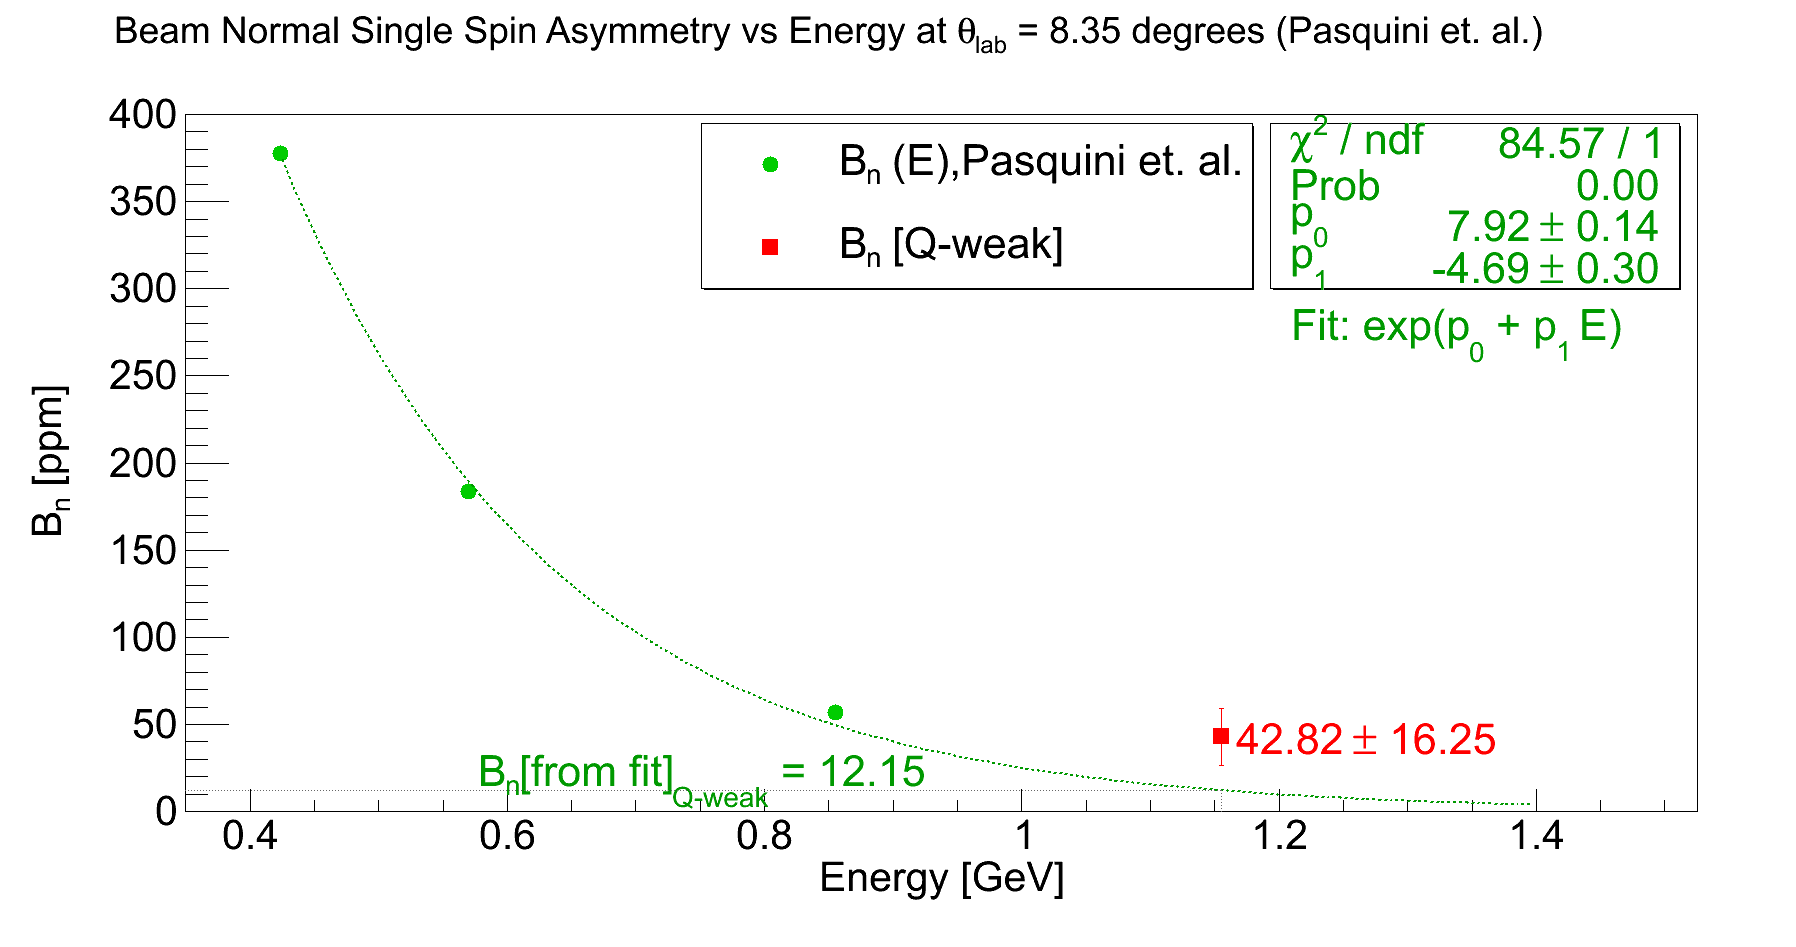
\includegraphics[width=15.0cm]{figures/theoryAsymmetryPasquiniEnergyDependence}
	\end{center}
	\caption
%	[BNSSA asymmetry calculation from Pasquini et al. and its extension.]
	{BNSSA asymmetry calculation from Pasquini et al. and its extension. The asymmetries from Figure~\ref{fig:theoryAsymmetryPasquini} at $\theta_{\rm lab}$ = 8.35\degrees{} are plotted here. A fit function of the form $f(E) = exp(p_{0}+p_{1}E)$ is used to extrapolate the asymmetry to the desired Q-weak kinematic region ($E$ = 1.155 GeV).}
	\label{fig:theoryAsymmetryPasquiniEnergyDependence}
\end{figure}


%%%%%%%%%%%%%%%%%%%%%%%%%%%%%%%%%%%%%%%%%%%%%%%%%%%%%%%%%%%%%%
%\section{BNSSA Leakage on Parity Violating Asymmetry}
%\label{BNSSA Leakage on Parity Violating Asymmetry}
%
%The BNSSA in electron-proton scattering can create false asymmetry into the parity violating asymmetry measurements when the azimuthal symmetry of the detector array is broken and for residual transverse polarization in the electron beam.
%
%The transverse measurement discussed in this chapter was used to determine to assign a systematic uncertainty for the parity violating asymmetry to take into account the false asymmetry generated by BNSSA.

%%%%%%%%%%%%%%%%%%%%%%%%%%%%%%%%%%%%%%%%%%%%%%%%%%%%%%%%%%%%%%
\section{BNSSA in LH$_{2}$ at Both Sides of the Inelastic Peak}
\label{BNSSA in LH$_{2}$ at Both Sides of the Inelastic Peak}

Data on both sides of the inelastic peak (at QTor current 6000~A and 7300~A) were taken to better constrain the elastic dilution. The same prescription was used, as described in section~\ref{Extraction of Physics Asymmetry}, to extract the off peak physics asymmetries. 
The measured five-parameter regressed asymmetries are $\epsilon_{M}^{6000A}$ = 7.198~$\pm$~0.688~(stat)~$\pm$~0.163~(sys)~ppm, and $\epsilon_{M}^{7300A}$ = 0.717~$\pm$~0.476~(stat)~$\pm$~0.252~(sys)~ppm at QTor current 6000~A, and 7300~A, respectively (more details about the systematic studies are in APPENDIX~\ref{Beam Normal Single Spin Asymmetry in Inelastic e-p Scattering}). 
Data were taken on the 4\% downstream aluminum alloy target to determine the background contributions to the measured asymmetry at QTor current 7300~A, but there was no measurement at 6000~A.
The measured regressed Al asymmetry at QTor current 7300~A is $\epsilon^{DSAl}_{M}$ = -0.108~$\pm$~1.083~(stat) $\pm$ 1.140~(sys)~ppm. After correcting for the acceptance difference between the upstream and downstream target windows, and the beam polarization, the background windows correction asymmetry becomes $B^{7300A}_{Al}$ = -0.120~$\pm$~1.791~ppm. A scaled Al windows asymmetry from the inelastic peak was used at 6000~A, where the LH$_{2}$ asymmetry was used to scale the Al asymmetry. The acceptance and polarization corrected asymmetry for windows correction is $B^{6000A}_{Al}$ = 12.937~$\pm$~2.709~ppm. The same dilution for the windows correction was used (see section~\ref{Target Aluminum Windows}) for both datasets. The correction from other neutral background, and beamline scattering were same as inelastic peak dataset. The same elastic asymmetry was used for both datasets, whereas the dilutions were obtained using simulation as $f_{el}^{6000A}$ = 0.732~$\pm$~0.095 and $f_{el}^{7300A}$ = 0.797~$\pm$~0.020. The discrepancy between the data and simulation was larger for the left side of the inelastic peak, as shown in Figure~\ref{fig:elasticDilutionDiscrepancy}, which contributed to the uncertainty in the dilution. The extracted beam normal single spin asymmetries at QTor current 6000~A and 7300~A are $B_{n}^{6000A}$ = 63.71 $\pm$ 4.45 (stat) $\pm$ 36.17 (sys)~ppm, and $B_{n}^{7300A}$ = 42.17 $\pm$ 5.26 (stat) $\pm$ 9.85 (sys)~ppm, respectively (see Figure~\ref{fig:asymmetryLH2_vs_QTor}).

\begin{figure}[!h]
	\begin{center}
	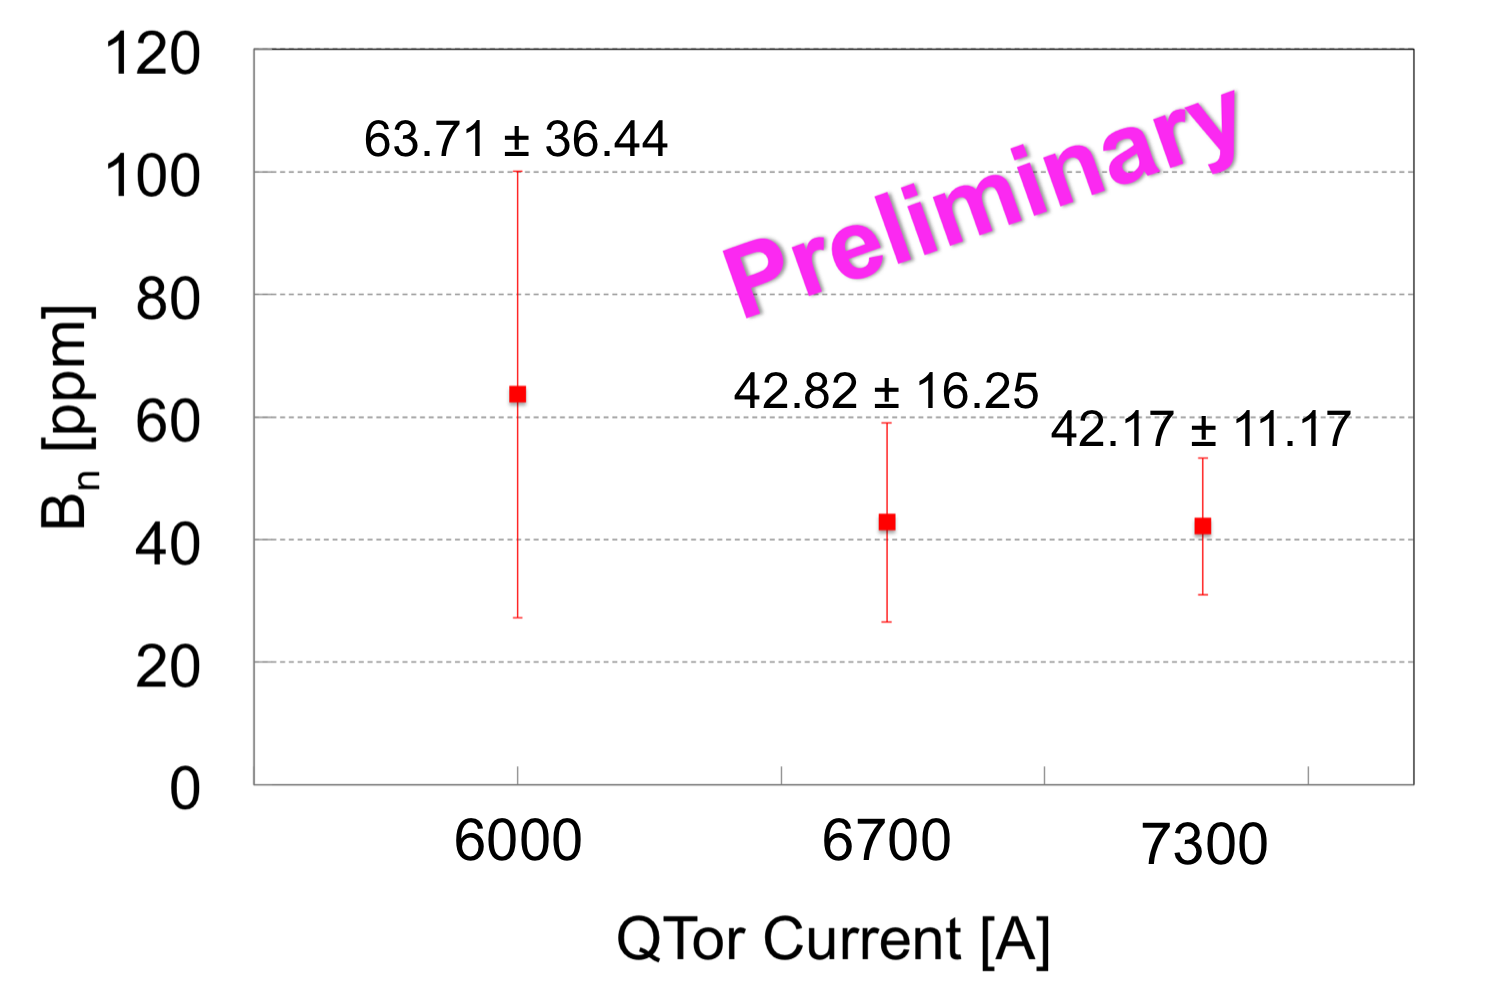
\includegraphics[width=15.0cm]{figures/asymmetryLH2_vs_QTor}
	\end{center}
	\caption
%	[BNSSA at N$\rightarrow\Delta$ peak and off peak asymmetries in LH$_{2}$.]
	{BNSSA at N$\rightarrow\Delta$ peak and off peak asymmetries in LH$_{2}$. The QTor current was changed to 6000~A, and 7000~A from 6700~A to cover the both sides of the N$\rightarrow\Delta$ peak. The missing mass, $W$, at the inelastic peak (6700~A) is 1.2~GeV. The uncertainty in the asymmetry is the total uncertainty and is the quadrature sum of the statistical and systematic uncertainties. The total uncertainty is dominated by the systematic uncertainty from elastic radiative tail.}
	\label{fig:asymmetryLH2_vs_QTor}
\end{figure}




%%%%%%%%%%%%%%%%%%%%%%%%%%%%%%%%%%%%%%%%%%%%%%%%%%%%%%%%%%%%%%
\section{BNSSA in Nuclear Targets}
\label{BNSSA in Nuclear Targets}

In this chapter, the inelastic beam normal single spin asymmetry measurements in e-p scattering have been discussed. In addition to the inelastic data from the proton, Q-weak has data on the beam normal single spin asymmetry measurements from several other physics processes. Few of these measurements are the first of their kind and carry interesting physics. The measured regressed five-parameter asymmetries on liquid hydrogen cell, 4\% thick downstream aluminum alloy, and a 1.6\% thick downstream carbon foil are summarized in Table~\ref{tab:transverse_inelastic_asymmetry_nuclear_target}. The relative statistical precision of the measurements are also shown. The analysis of these data is ongoing and expected to test model calculations of beam normal single spin asymmetry.


%\renewcommand{\arraystretch}{1.5} % make cell wider
%\begin{table}[!h]
% \begin{center}
%   \caption
%	[Measured regressed (5+1) asymmetries in inelastic electron-nucleon scattering for transverse polarized beam.]
%   {Measured regressed (5+1) asymmetries in inelastic electron-nucleon scattering for transverse polarized beam. Horizontal and vertical transverse data set are shown separately. The combined (error weighted average) asymmetries are also noted. The inelastic peak is at QTor current 6700~A. The other QTor currents were taken to improve the simulation for elastic radiative tail.}
%  \begin{tabular}{ c | c | c  c  c | c  c }
%%    \hline
%    \noalign{\hrule height 1pt}
%    \multirow{4}{*}{Pol.} & \multicolumn{6}{c}{Asymmetry [ppm]} \\ 
%   	\cline{2-7}
%    & \multicolumn{6}{c}{QTor currents} \\ 
%   	\cline{2-7}
%%	\hline
%	& 6000 A & & 6700 A & &  \multicolumn{2}{c}{7300 A}\\
%	\cline{2-7}%
%%	\hline
%	& LH$_{2}$ & LH$^{\dagger}_{2}$ & Al$^{\dagger\dagger}$ & $^{12}$C &  LH$_{2}$ & Al \\
%%	\cline{2-7}%\hline
%    \noalign{\hrule height 1pt}
%%    \hline
%%	Hor. & \pbox{2cm}{7.212$\pm$0.688} & \pbox{2cm}{(4.525$\pm$0.806)\\ 5.343$\pm$0.532} & \pbox{2cm}{(9.631$\pm$1.768)\\ 7.892$\pm$1.186} & \pbox{2cm}{10.190$\pm$1.863} & \pbox{1.8cm}{0.967$\pm$0.477} & \pbox[c][2cm][c]{2cm}{-1.245$\pm$1.087} \\ 
%	Hor. & 7.212$\pm$0.688 & 5.343$\pm$0.532 & 7.892$\pm$1.186 & 10.190$\pm$1.863 & 0.967$\pm$0.477 & -1.245$\pm$1.087 \\
%	Ver. &  & 4.525$\pm$0.806 & 9.631$\pm$1.768 & & & \\ 
%    \hline
%	\multirow{2}{*}{Both} & 7.212$\pm$0.688 & 5.095$\pm$0.444 & 8.432$\pm$0.985 & 10.190$\pm$1.863 & 0.967$\pm$0.477 & -1.245$\pm$1.087 \\
%	 & (9.5\%) & (8.7\%) & (11.7\%) & (18.3\%) & (49.3\%) & (87.3\%) \\
%%    \noalign{\hrule height 1pt}
%%	   Beam current $I$ [$\mu$A] & 180 & 180 & 60 & 75 & 180 & 60 \\
%    \noalign{\hrule height 1pt}
%   \end{tabular}
% \label{tab:transverse_inelastic_asymmetry_nuclear_target}
% \end{center}
%\end{table}
%\renewcommand{\arraystretch}{1.0} % make cell wider


\begin{table}[!h]
 \begin{center}
   \caption
%	[Measured regressed five-parameter asymmetries in inelastic electron-nucleon scattering for transverse polarized beam.]
   {Measured regressed five-parameter asymmetries in inelastic electron-nucleon scattering for transverse polarized beam. Horizontal and vertical transverse data set are shown separately. The combined (error weighted average) asymmetries are also noted. The inelastic peak is at QTor current 6700~A. The other QTor currents were taken to improve the simulation for elastic radiative tail. The first uncertainty represents statistical contribution, whereas second represents systematic contribution. The missing mass, $W$, at the inelastic peak (6700~A) is 1.2~GeV.}
  \begin{tabular}{ c | c | c | c }
%    \hline
    \noalign{\hrule height 1pt}
    \multirow{4}{*}{Pol.} & \multicolumn{3}{c}{Asymmetry [ppm]} \\ 
   	\cline{2-4}
    & \multicolumn{3}{c}{QTor currents} \\ 
   	\cline{2-4}
%	\hline
	& 6000~A & 6700~A & 7300~A \\
%	\cline{2-4}%
    \noalign{\hrule height 1pt}
    \multicolumn{4}{c}{LH$_{2}$} \\
    \hline
	Hor. & 7.198 $\pm$ 0.688 $\pm$ 0.163 & 5.303 $\pm$ 0.533 $\pm$ 0.092 & 0.717 $\pm$ 0.476 $\pm$ 0.252 \\
	Ver. & & 4.457 $\pm$ 0.807 $\pm$ 0.117 & \\ 
    \hline
	\multirow{2}{*}{Both} & 7.198 $\pm$ 0.688 & 5.047$ \pm$ 0.444 & 0.717 $\pm$ 0.476 \\
	 & (9.5\%) & (8.7\%) & (49.3\%)\\
    \noalign{\hrule height 1pt}
    \multicolumn{4}{c}{Al} \\
    \hline
	Hor. & 	& 7.911 $\pm$ 1.187 $\pm$ 0.482	& -0.108 $\pm$ 1.083 $\pm$ 1.140 \\
	Ver. & 	& 9.533 $\pm$ 1.759 $\pm$ 0.870	& \\ 
    \hline
	\multirow{2}{*}{Both} & & 8.419 $\pm$ 0.984 $\pm$ 0.603 & -0.108 $\pm$ 1.083 $\pm$ 1.140 \\
	&  & (11.7\%) & (87.3\%) \\
    \noalign{\hrule height 1pt}
    \multicolumn{4}{c}{$^{12}$C} \\
    \hline
	\multirow{2}{*}{Hor.} & & 9.869 $\pm$ 1.870 $\pm$ 0.549 &  \\
	&  & (18.3\%) &  \\
    \noalign{\hrule height 1pt}
   \end{tabular}
 \label{tab:transverse_inelastic_asymmetry_nuclear_target}
 \end{center}
\end{table}



%%%%%%%%%%%%%%%%%%%%%%%%%%%%%%%%%%%%%%%%%%%%%%%%%%%%%%%%%%%%%
\section{Conclusion}
\label{Conclusion}

The Q-weak collaboration has made a 35\% relative measurement of the beam normal single spin asymmetry of $B_{n} = 42.82\pm2.45~\text{(stat)}\pm16.07~\text{(sys)}~\text{ppm}$ using transversely polarized 1.155~GeV electrons scattering in-elastically from protons with an average $Q^{2}$ of 0.0209~(GeV/c)$^{2}$, an average scattering angle of 8.3\degrees{}, and missing mass of 1.204~GeV. This is the first measurement of the beam normal single spin asymmetry in inelastic electron-proton scattering. This measurement would be an excellent test of theoretical calculations. Unfortunately, at the time of this analysis, there was no existing theoretical calculation or model to compare with the data. Hopefully this thesis will encourage theoreticians to produce new calculations. 

%Going further, Qweak beam normal single spin asymmetry measurements can be used to estimate the real part of the two-photon exchange with the use of dispersion relations. This will provide a valuable cross-check of both the dispersion relations and the models of the real part of the two-photon exchange process.